\hypertarget{group__group13}{
\chapter{Functional Overview}
\label{group__group13}
}

\begin{flushleft}
The ASP COR service provides interfaces to access, modify and manage the life cycle of objects. These objects are called Managed Objects as they contain 
management information about network elements such as a Chassis. They are used to exchange information between system management 
applications and applications running on network elements. The applications running on a network element use or produce management information.
COR objects and metadata associated with these Managed Objects are located in an in-memory object storage.  
\par
System Management Applications reside outside the network and use the services of a local management agent to interface with COR. These local agents are
referred to as Object Managers (OM).
\par
Applications in a network element that use or produce the management information are referred to as Object Implementers.
An ASP Service can act as an Object Implementer for an object of interest.
\par
Object Manager and Object Implementer are roles performed by applications. In the current implementation of COR, COR is unaware of Object 
Manager and Object Implementer roles and does not enforce any semantics related to these roles. It is assumed that the OM and OI roles
are maintained by careful application design.        
\par
Currently, COR does not provide support for system management applications to use their own agents while interacting with network elements.
Management agents would need to gain exclusive control of a set of managed objects temporarily to perform some change. In the current implementation, it 
is assumed that multiple Object Managers, if present, co-operate with each other while managing or making changes to objects.

\chapter{Service Model}
\section{Usage model}
Applications can model their network elements and represent them as COR Information Model. These applications can use MO classes and the 
containment relationship in COR to interpret the relationship between various network elements.

\begin{description}
\item
[Management Applications (North-bound)]
Management application can perform CREATE, DELETE or SET operations on Managed Objects for configuration purposes. Management applications can also subscribe
to CREATE, DELETE or MODIFY notifications on Managed Objects. Such Managed Objects reflect the status of associated network elements.

\item[Object Implementor]
An Object Implementer (OI) implements the configuration supplied by the north bound. An OI can also perform CREATE, DELETE, and MODIFY operations 
on Managed Objects to reflect its run-time status. 

\end{description}
\section{Functional Description}
\subsection{Managed Object Class Characteristics}
\subsubsection{COR MO-Class and MSO-Class}

A MO COR-class is a collection of attributes. Each class has a name and an integral identifier. An MO-class has two services associated with it:
\begin{itemize}
\item
Provisioning service 
\item
Alarm service
\end{itemize}

COR groups related attributes of these two services in two different Managed Service Object Class (also called MSO class).
Thus, an MO class has two different MSO classes. One corresponding to Provision-able attributes and the other corresponding to Alarm 
attributes. The MSO class also has a name and a list of attributes.
\par
ASP Alarm service determines the structure of the Alarm MSO class and uses this class to model alarms. 
\par
The Provision-able MSO class structure is defined by the application. From the modeling perspective, it is only the PROV MSO class that is of interest 
to the application. For example, a GigePort class can have a group of provisionable attributes (MTU size) and a group of alarms (such as LOS, LOF
and so on).
COR considers these two groups as two distinct MSO classes associated with GigePort class. An MSO class is identified by an MO class and its Service ID 
The Service ID indicates if the MSO is Provisionable or corresponding to Alarm. The enumeration, {\tt{ClCorServiceIdT}}, specifies the service ID of a class.

\subsubsection{MO tree and Containment}

All Managed Objects in COR are organized in a tree hierarchy called the MO tree. The relationship of an MO to its parent MO in the hierarchy is referred 
to as its "containment" relationship. An MO can only be contained in MOs belonging to other MO classes. The rules related to permitted containment relations 
are part of the definition of an MO Class.

\par
The containment relationship allows COR to organize all MOs in a tree and is therefore mandatory from COR's perspective.
Containment relationship is of no other significance to COR. However, it can have some special significance to management applications as some OIs 
can be interested in a group of related objects (in a subtree). For example, a subtree could reflect the containment of the 
Availability Management Service (AMS) related objects and this containment can have special significance to AMS.

\subsubsection{Blueprint for the MO Tree}

The MO Class definitions and the permitted containment relations in COR are also referred to as the "blueprint" for the MO tree. This blueprint 
refers to the complete set of object metadata associated with a COR instance. COR permits objects to be created and attached to a tree according to the 
blueprint. This blueprint can be constructed using the OpenClovis Integrated Development Environment (IDE). The blueprint is exported in the COR XML
file and imported by COR when it is initialized for the first time. The blueprint is kept in the COR's persistent storage referred to as COR-DB. 
COR obtains the blueprint from COR-DB during its subsequent startup.

\subsection{MO Attributes}
\subsubsection{Attribute Characteristics}
Each MO attribute has the following characteristics:
\begin{itemize}
\item
Name
\item
Type associated with attribute values
\item
Default value
\item
Qualifier
\item
Sub qualifiers
\end{itemize}
The qualifiers supported are:
\begin{itemize}
\item
Config
\item
Run-time
\end{itemize}

The sub-qualifiers supported are:
\begin{itemize}
\item
Cached
\item
Persistent
\item
Initialized
\item
Writable
\end{itemize}

\subsubsection{Attribute Types Supported}
\begin{Desc}
\item[Integer and String Types]\end{Desc}

The supported types are signed and unsigned integers of various sizes. Arrays of these integer types are also supported.  For integer types, 
a maximum, minimum, and default value can be specified.


\subsubsection{Caching and Persistence of COR objects}
All COR metadata and objects are persisted in the COR-DB. However, the attribute values are not always persisted. This control can be exercised at 
the object attribute level. Persisted object attributes are restored in a COR instance automatically after a GMS-Cluster reboot.
\par 
COR stores the values of attribute in the memory. This is referred to as caching. Caching results in better read access times for cached attributes. Caching of 
data is not required when the cached data can quickly become stale. Controls are provided to prevent caching of this type of data. These are explained in
subsequent sections.  

\subsubsection{Attribute Qualifiers}
Every attribute must be qualified as a CONFIG, run-time or KEY. These qualifiers are mutually exclusive.


\begin{Desc}
\item
[Configuration Attributes]
A configuration attribute is always persisted and cached. Configuration attributes contain data provided by the Object Managers. They are read-only from
the perspective of the Object Implementer.

\end{Desc}


\begin{Desc}
\item[Run-time Attributes]
A run-time attribute is not persisted or cached by default. The following sub-qualifiers (either singly or in any combination) can be associated with a 
run-time attribute:
\begin{itemize}
\item
Persistent - This sub-qualifier for run-time attributes indicates that the attribute must be made persistent by the COR Service.
\item
Cached - This sub-qualifier for run-time attribute indicates that the attribute must be cached by the COR service.
\end{itemize}
Run-time attributes are used for data provided by Object Implementers. They are read only from an Object Manager's perspective.
A run-time attribute that is cached is updated by the Object Implementer when the value changes. When a read request is made on such a run-time attribute, 
COR reads the value from the cache.
A read request on a run-time attribute that is not cached triggers a synchronous request to the Object Implementer that returns with the value of the
attribute.
\par
For examples:\par
{\tt{run-time + cached ->}} Attribute showing Application log stream file name implemented by the Log service.
\par
{\tt{run-time + cached + persistent ->}} Administrative state of a service unit implemented by AMF.
\par
{\tt{run-time + multi-valued ->}} List of Service Instances currently assigned to a Service Unit, implemented by AMF.

\end{Desc}

\subsection{Object Addressing}
\subsubsection{MOID}

Every object in the COR MO tree has a unique ID referred to as the MOID (Managed Object ID).
Every object has a {\tt{relative\_\-ID}} that is formed from the tuple, {\tt{class\_\-ID}} and {\tt{instance\_\-ID}}, where:
\begin{itemize}
\item
class\_\-ID - uniquely identifies the MO class of which this object is an instance and 
\item
instance\_\-ID - uniquely identifies this instance of the object from other instances having the same parent.
\end{itemize}
The MOID of an object is formed from the tuple, MOID of the parent and {\tt{relative\_\-ID}} of the object.
For example, an AMF Service Unit instance can have the following MOID: 
{\tt{COR\_\-ROOT\_\-CLASS\_\-ID:0/APPLICATION\_\-CLASS\_\-ID:0/SERVICE\_\-GROUP\_\-CLASS\_\-ID:1/SERVICE\_\-UNITCLASS\_\-ID:3}}
\par
COR provides APIs to manage the life cycle of an object and to read or modify its attributes. The user is required to know the MOID of the 
object or its parents.
\par
A MOID uniquely identifies an object in COR tree. However, a variant of the MOID is also used to specify ranges of objects. These are called wild card 
MOIDs. A wild card {\tt{class\_\-ID}} can represent any class and a wild card {\tt{instance\_\-ID}} can represent any instance. The wild card MOID 
is used for OI subscription and for specifying an MO instance search criteria. Following are some of the examples of a wild card MOID:
\begin{itemize}
\item
{\tt{COR\_\-ROOT\_\-CLASS\_\-ID:0/APPLICATION\_\-CLASS\_\-ID:0/SERVICE\_\-GROUP\_\-CLASS\_\-ID:1/SERVICE\_\-UNITCLASS\_\-ID:*}}\par
Specifies all the MO instances of {\tt{SERVICE\_\-UNITCLASS\_\-ID}} class under the hierarchy. \par
{\tt{COR\_\-ROOT\_\-CLASS\_\-ID:0/APPLICATION\_\-CLASS\_\-ID:0/SERVICE\_\-GROUP\_\-CLASS\_\-ID:1}}
\item
{\tt{COR\_\-ROOT\_\-CLASS\_\-ID:0/APPLICATION\_\-CLASS\_\-ID:0/SERVICE\_\-GROUP\_\-CLASS\_\-ID:1/*:*}}\par
Specifies all the MO instance of any class under the hierarchy.\par
{\tt{COR\_\-ROOT\_\-CLASS\_\-ID:0/APPLICATION\_\-CLASS\_\-ID:0/SERVICE\_\-GROUP\_\-CLASS\_\-ID:1}}
\item
{\tt{COR\_\-ROOT\_\-CLASS\_\-ID:0/APPLICATION\_\-CLASS\_\-ID:0/SERVICE\_\-GROUP\_\-CLASS\_\-ID:*/*:*}}\par
Specifies all the MO instance of any class under the subtree {\tt{COR\_\-ROOT\_\-CLASS\_\-ID:0/APPLICATION\_\-CLASS\_\-ID:0/SERVICE\_\-GROUP\_\-CLASS\_\-ID:*.}}\par
The subtree specified by {\tt{COR\_\-ROOT\_\-CLASS\_\-ID:0/APPLICATION\_\-CLASS\_\-ID:0/SERVICE\_\-GROUP\_\-CLASS\_\-ID:*}} covers all the MO instances\par
of {\tt{SERVICE\_\-GROUP\_\-CLASS\_\-ID under COR\_\-ROOT\_\-CLASS\_\-ID:0/APPLICATION\_\-CLASS\_\-ID:0/}}
\end{itemize}


\subsection{Object Management Interfaces}
\begin{Desc}
\item
[OI and Primary OI]\end{Desc}
An Object Implementer performs several distinct operations in relation to changes in objects that include: 
\begin{itemize}
\item
Permits or denies an object creation or deletion request.
\item
Permits or denies changes to a configuration attribute value.
\item
Implements a change in a configuration attribute when the change has occurred in COR.
\item
Asynchronously updates a cached runtime attribute in COR as and when the related variable changes internally.
\item
Synchronously provides the value of a (non cached) run-time attribute when requested by COR.
\end{itemize}
Every object can have one or more object implementers. While multiple OIs can perform the first three activities, there can be only one OI that is 
allowed to perform the last two activities. 

\begin{Desc}
\item
[OI Registration]\end{Desc}
A component can act as an OI for an MO as specified in a wild card MOID. For example,
\begin{itemize}
\item
An MO Instance specified through its MoID. For example, the MoID can be 
\par
COR\_\-ROOT\_\-CLASS\_\-ID:0\/APPLICATION\_\-CLASS\_\-ID:0\/SERVICE\_\-GROUP\_\-CLASS\_\-ID:1\/SERVICE\_\-UNITCLASS\_\-ID:1\/
\item
Instances of a particular MO Class hanging from a particular hierarchy. 
\par
COR\_\-ROOT\_\-CLASS\_\-ID:0\/APPLICATION\_\-CLASS\_\-ID:0\/SERVICE\_\-GROUP\_\-CLASS\_\-ID:1\/SERVICE\_\-UNITCLASS\_\-ID:*
\item
A complete subtree. A Component can specify itself as the OI for the wild card
\par
COR\_\-ROOT\_\-CLASS\_\-ID:0\/APPLICATION\_\-CLASS\_\-ID:0\/SERVICE\_\-GROUP\_\-CLASS\_\-ID:*\/SERVICE\_\-UNITCLASS\_\-ID:*
\end{itemize}
As a component can act as an OI for multiple MO instances corresponding to different MO classes, COR provides a mechanism to associate an OI callback 
APIs for each MO class.
\par
The OI and MO association is performed during modeling. The following table provides a list of OI callback APIs provided by COR.
\begin{tabular}{|l|l|p{4in}|}
\hline
 {\bf No.} & {\bf OI Callback Function} & {\bf Description} \\
\hline
         1 & Constructor & COR invokes this function when an MO is required to be created.  An application can embed its custom logic to implement
         MO creation. Currently, MO creation/deletion does not have a validate callback function. \\
\hline
         2 & Destructor & COR invokes this callback when an MO is required to be deleted.  An application can embed its custom logic to implement MO
         deletion. Currently, MO creation/deletion does not have a validate callback function. \\
\hline
         3 & Validate & COR invokes this callback to validate the attribute that is being SET. The callback either permits or denies the application 
         containing this attribute. The semantics of validation is specific to the OI. An OI can acquire resources (such as memory) required to
         APPLY this attribute to ensure that the APPLY operation is successful. This pre-acquisition reduces the possibility of
         failure of APPLY operation. \\
\hline
         4 & Rollback & This callback is invoked when the validate operation fails on this attribute or validate fails on another attribute that is part of 
         the transaction. This callback allows the OI to free any pre-allocated resources, acquired in the validate phase. The rollback API is called if 
         any other operation that is part of this transaction fails to validate.  \\
\hline
         5 & Apply & This function applies the attribute to the resource. \\
\hline
\end{tabular}  


\begin{Desc}
\item
[COR Session Capability]\end{Desc}
The COR session capability provides a mechanism to execute a group of jobs (CREATE, DELETE and MODIFY operations on a MO) in an efficient manner by minimizing the number of RMD calls between the COR 
client, COR server, and Object Implementer. The COR session capability provides a mechanism to execute CREATE, SET, and DELETE operations on a group of MOs with
all-or-none semantics as described in this section.
\par
The COR server performs a basic validation on these jobs. If one of the job validation fails, the session becomes invalid and no
operations are performed.

\par
COR determines the OI for each participating MO, and invokes the validate callback of the OI. If the OIs successfully validate
their MO operation, COR invokes the apply APIality of the OI. COR also internally updates its database with these changes on the MOs. On successful
completion, COR sends a notification for the changed MOs.
\par
If an OI fails validation, COR does not proceed with the apply. COR determines the set of OIs that have completed validation and calls 
the rollback APIs.
\par
The following sequence diagrams describe the control flow between COR-client, COR-server, and OIs for the following two cases. 
\begin{itemize}
\item
A session is initiated by \textit{comp1}. In the session \textit{<mod1,attr1>} ,\textit{<moid2,attr2>} and \textit{<moid3,attr3>} are getting updated.
\item
Both \textit{comp1} and \textit{comp2} are OIs for \textit{<moid1>} ,\textit{<moid2>}, and \textit{<moid2>}.
\item
All OIs have the same callback API name. The name of the validate, rollback, and apply callbacks are {\tt{oiValidateFxn}}, {\tt{oiRollbackFxn}}, and 
{\tt{oiApplyFxn}}. 
\item
Case 1:
\begin{itemize}
\item
Both OIs validate \textit{<moid1,attr1>}, \textit{<moid2,attr2>}, and \textit{<moid3,attr3>} successfuly.
\item
Thus, the apply of these attributes is successful.
\end{itemize}

\item
Case2:
\begin{itemize}
\item
\textit{comp1} successfuly validates \textit{<moid1,attr1> ,<moid2,attr2>}, and \textit{<moid3,attr3>}.
\item
\textit{comp2} successfuly validates \textit{<moid1,attr1>} and fails validation in \textit{<moid2,attr2>}. A rollback can now be called.
\item
Rollback is called for \textit{comp1} for the attributes: \textit{<mod1,attr1>}, \textit{<moid2,attr2>}, and \textit{<moid3, attr3>}.
\item
Rollback is called for \textit{comp2} for the attributes: \textit{<moid1,attr1>} and \textit{<moid2,attr2>}.
\item
No attributes are applied.
\end{itemize}
\end{itemize}
\end{flushleft}
\newpage
\begin{center}
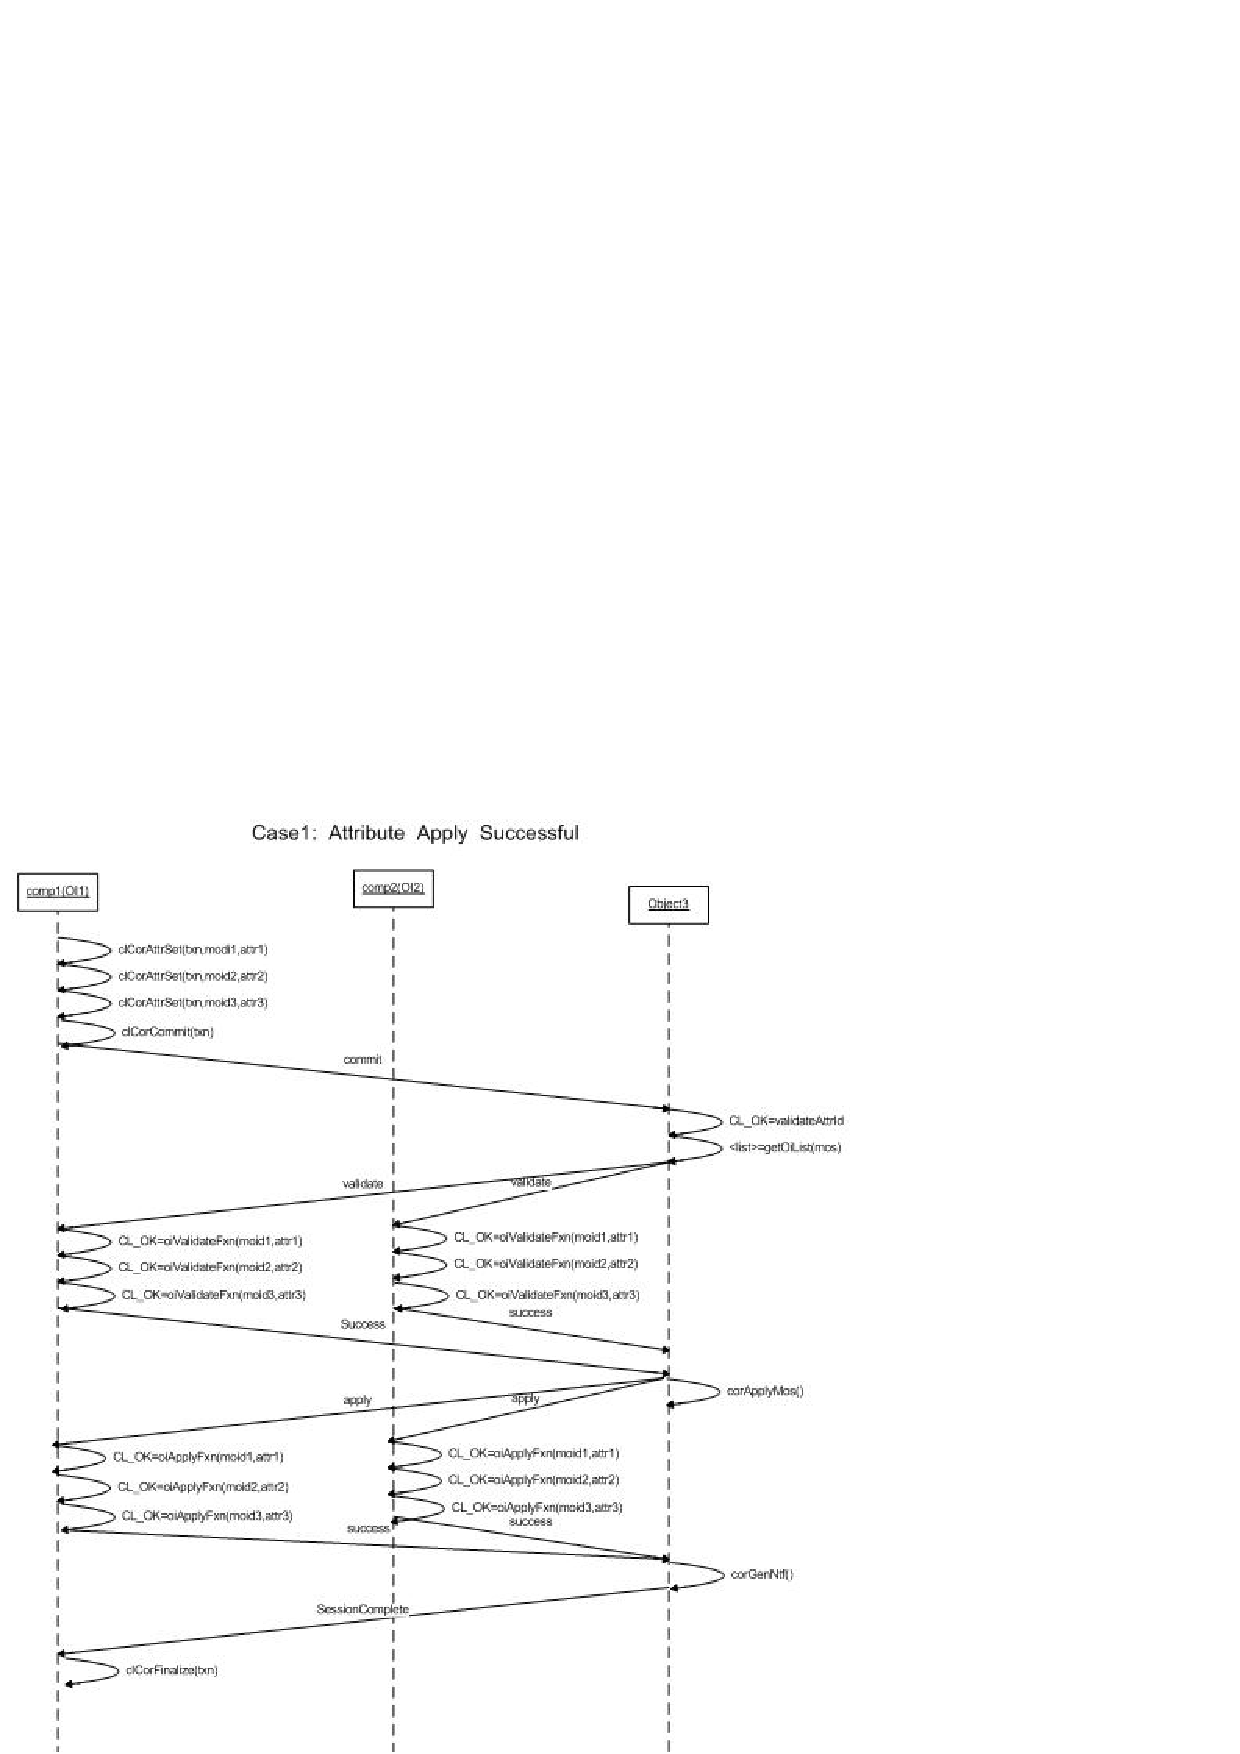
\includegraphics{cor1.jpg}
\end{center}

\newpage
\begin{center}
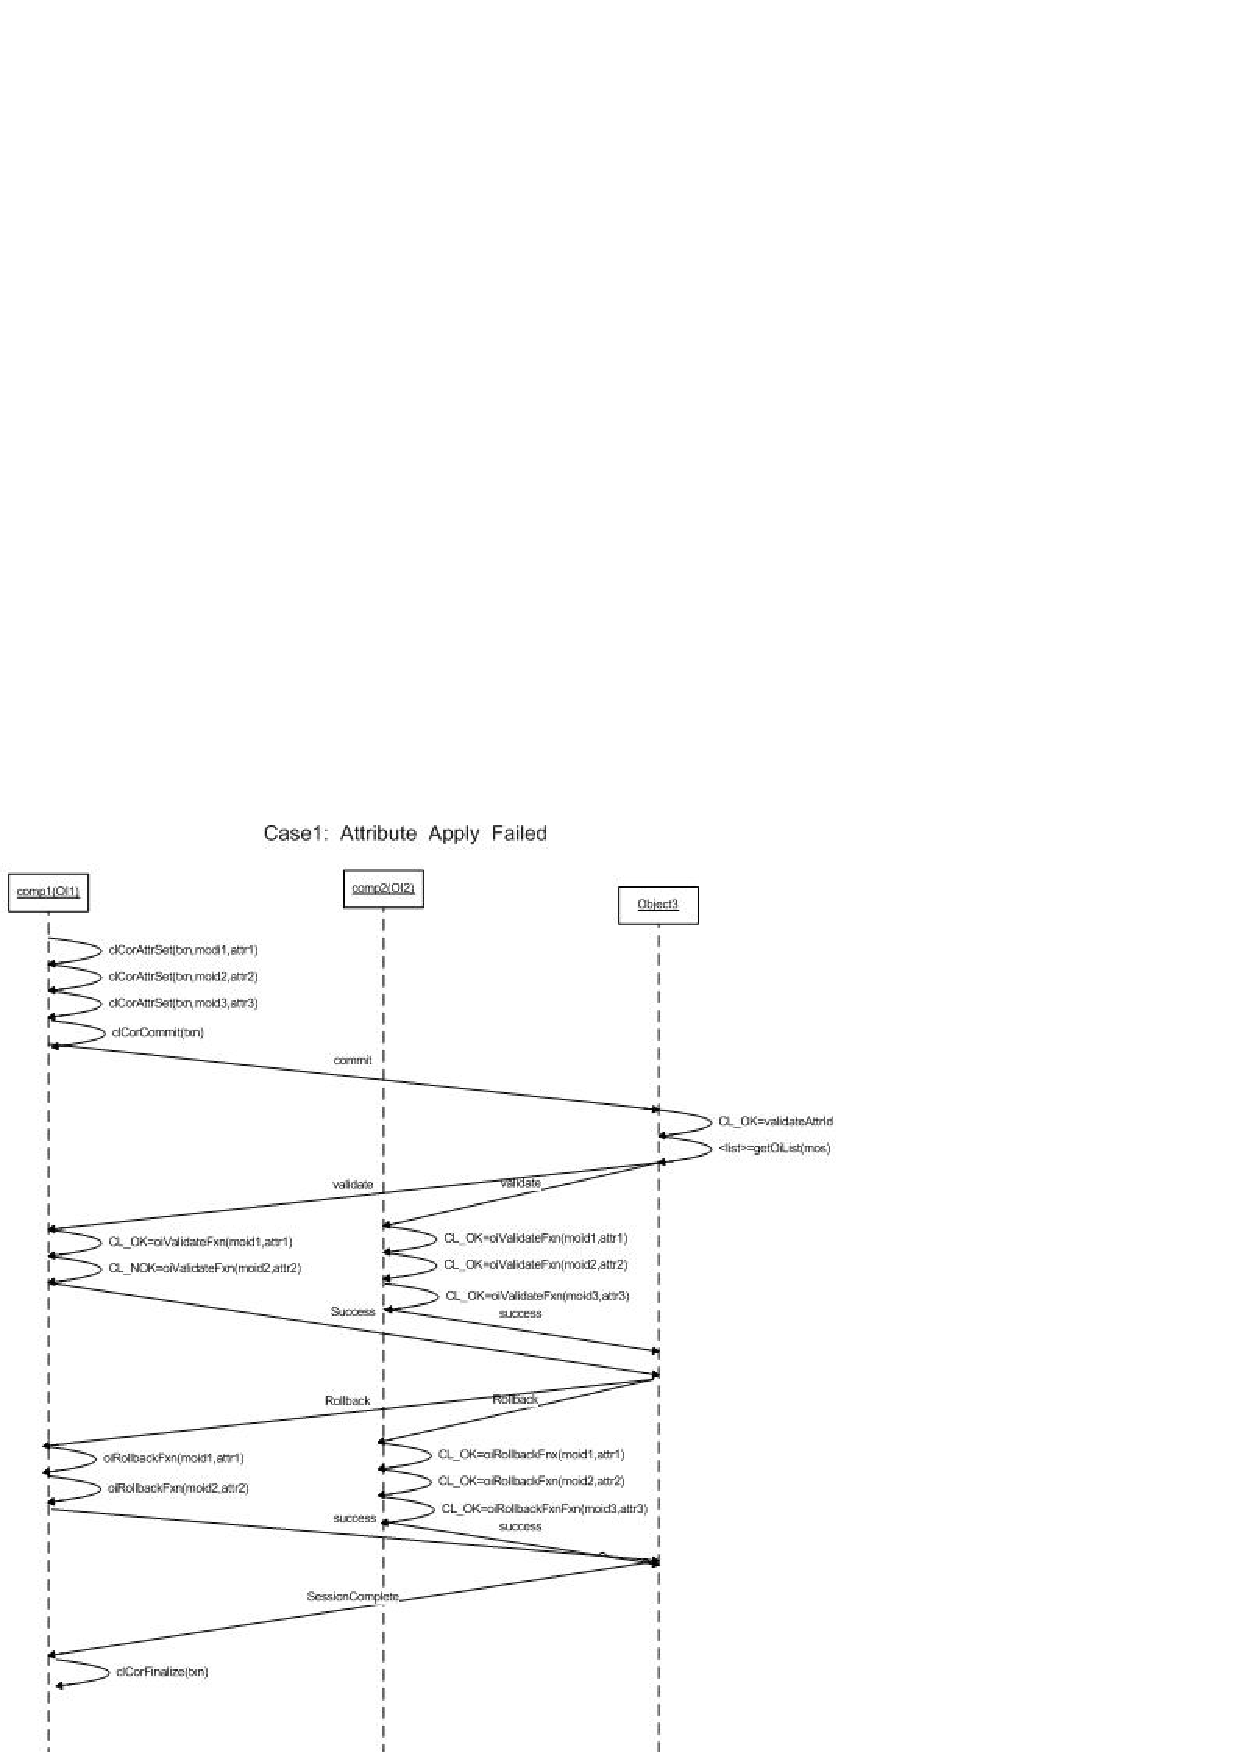
\includegraphics{cor2.jpg}
\end{center}



\begin{flushleft}
\begin{Desc}
\item
[COR Bundle Capability]\end{Desc}
The COR bundle capability provides a mechanism to execute groups of attribute reads in an efficient manner by minimizing the number of RMD calls between 
COR client, COR server, and Object Implementer.  
\par
A bundle is non-transactional in nature. A non-transactional bundle can contain attributes that are not successfully read. 
\par
The bundle semantics of executing jobs is performed in four phases by the application:
\begin{enumerate}
\item
Bundle Creation - A bundle is empty with no jobs associated when it is created. A bundle handle that identifies this bundle is returned.
\item
Job Population -  In the next phase, jobs are added to the bundle. A job corresponds to an MO and list of attributes that needs to be read. 
Multiple jobs consisting of different MOs can be a part of a bundle. These jobs are queued at the COR client. Every job has a status and
a buffer descriptor. The buffer descriptor contains the value of the attribute to be {\tt{set}} or {\tt{get}}. The success or failure of jobs 
 execution is reflected in the status.

\item
Bundle Apply - The application performs the APPLY operation synchronously when the population phase is completed. The bundle is submitted to the COR 
server that reads the value from the database or contacts the OI to obtain the value. The values are streamed back to the COR client at the end of 
this call.  

\item
Bundle Finalize - This frees up the resources allocated in bundle operation.
The following sequence diagram explains the control flow between COR client, COR server and OIs for the given case. 
\begin{itemize}
\item
A bundle operation is initiated by comp1. The bundle contains jobs: <mod1, attr1>,<moid2,attr1>, and <moid2,attr2>. <moid1, attr1> , 
<moid2,attr1> are run-time attributes.  
\item
These jobs are submitted by comp1.
\item
COR determines the PrimaryOI for moid1 and moid2 as <CompOI1> and <CompOI2>.
\item
COR obtains the values the run-time attributes of CompOI1 and CompOI2 for <moid1,attr1> and <moid2,attr1>.
\item
COR obtains the Config attribute value from its database. 
\item
COR returns back the value to comp1.
\end{itemize}

\end{enumerate}
\end{flushleft}
\newpage
\begin{center}
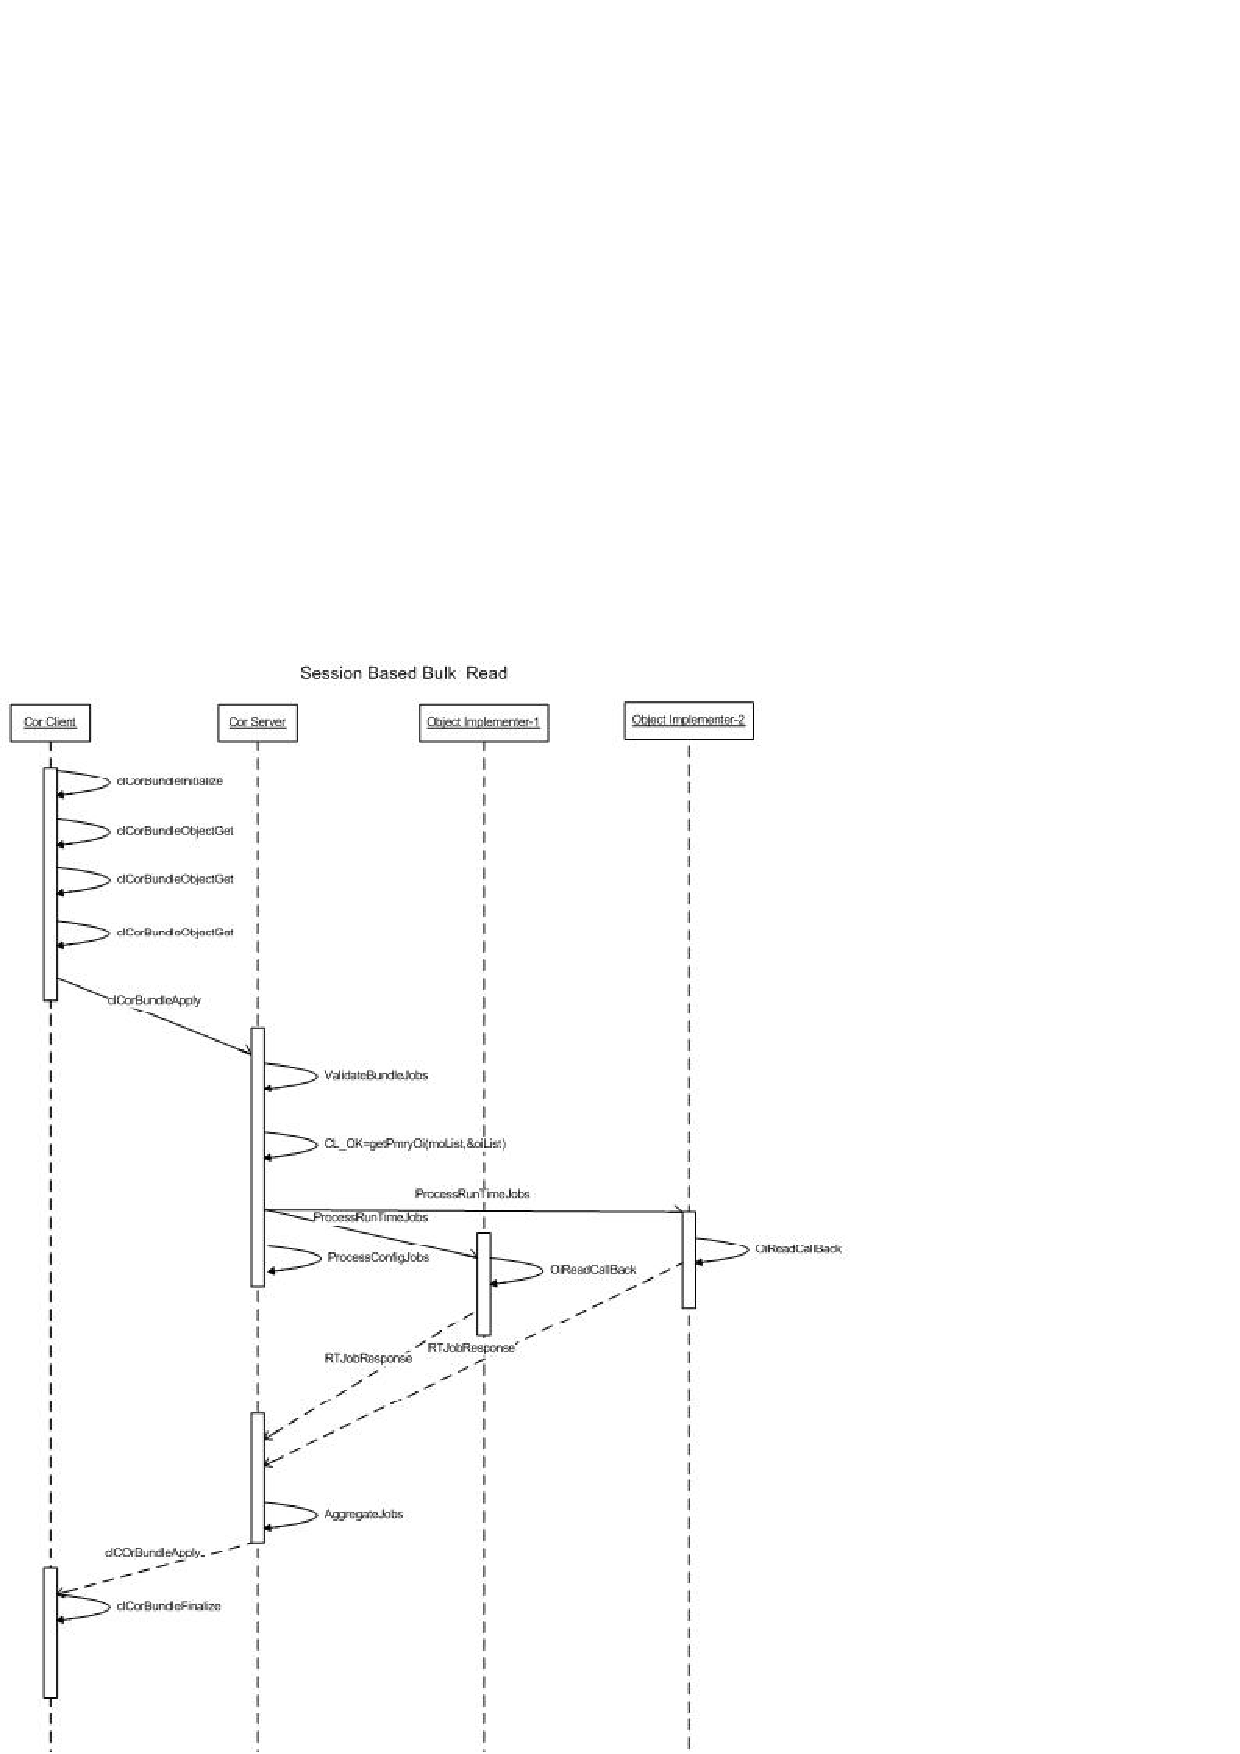
\includegraphics{cor3.jpg}
\end{center}

\begin{flushleft}

\begin{Desc}
\item
[COR Search Capability]\end{Desc}
COR provides the capability to retrieve objects matching a particular criterion. This criterion is called the filter and the search is termed as 
object-walk based search. Following are the parameters for this search:
\begin{itemize}
\item
Root - The root from where search needs to commence. The root is specified as MOID.
\item
Containment Tree - The subtree on which the search needs to be performed. This subtree is specified using wild-card MOID.
\item
Callback function - This is executed for each matched MO instance.
\end{itemize}
COR provides a mechanism to filter objects based on the value of their attributes. This search is called attribute-walk search.
This search is used in conjunction with object-walk search. 
Object-walk returns all the MO instances that match a particular search criterion. Each of these instance can be filtered based on a particular 
attribute and its value. Following are the parameters for this search:
\begin{itemize}
\item
MO - The MO tree on which the search is required to be performed.
\item
Attribute and its value - This is required to be compared.
\item
Callback function - This is required to be called when the attribute comparison is successful. 
\end{itemize}

\begin{Desc}
\item
[COR Event Generation and Subscription]\end{Desc}
COR generates an event for every object creation/deletion/set operation on the {\tt{COR\_\-EVT\_\-CHANNEL}}. Subscribing applications can specify the 
following filters to narrow down their event of interest.
\begin{itemize}
\item
MoID: Specifies the set of objects which is of interest to the application. The MoID can be a wild card MoID.
\item
Operation: Specifies the operation(s) that is of interest to the application. An operation can be a combination of Object-create, Object-delete, and 
Object-set activities.
\item
AttributeId: This specifies the attribute of interest. An application callback is executed when an event matching the filter is detected. 
\end{itemize}





\chapter{Service APIs}



\section{Error Definitions}
\index{Defines@{Defines}}

\begin{CompactItemize}

\item \# define CL\_\-COR\_\-ERR\_\-BUFFER\_\-OVERRUN (CL\_\-COR\_\-SET\_\-RC(CL\_\-ERR\_\-BUFFER\_\-OVERRUN)) 
\item \# define CL\_\-COR\_\-ERR\_\-BUNDLE\_\-APPLY\_\-FAILURE (CL\_\-COR\_\-SET\_\-RC(CL\_\-COR\_\-BUNDLE\_\-ERR\_\-MAX + 3)) 
\item \# define CL\_\-COR\_\-ERR\_\-BUNDLE\_\-FINALIZE (CL\_\-COR\_\-SET\_\-RC(CL\_\-COR\_\-BUNDLE\_\-ERR\_\-MAX + 6)) 
\item \# define CL\_\-COR\_\-ERR\_\-BUNDLE\_\-IN\_\-EXECUTION (CL\_\-COR\_\-SET\_\-RC(CL\_\-COR\_\-BUNDLE\_\-ERR\_\-MAX + 8)) 
\item \# define CL\_\-COR\_\-ERR\_\-BUNDLE\_\-INIT\_\-FAILURE (CL\_\-COR\_\-SET\_\-RC(CL\_\-COR\_\-BUNDLE\_\-ERR\_\-MAX + 2)) 
\item \# define CL\_\-COR\_\-ERR\_\-BUNDLE\_\-INVALID\_\-TYPE (CL\_\-COR\_\-SET\_\-RC(CL\_\-COR\_\-BUNDLE\_\-ERR\_\-MAX + 9)) 
\item \# define CL\_\-COR\_\-ERR\_\-BUNDLE\_\-TIMED\_\-OUT (CL\_\-COR\_\-SET\_\-RC(CL\_\-COR\_\-BUNDLE\_\-ERR\_\-MAX + 7)) 
\item \# define CL\_\-COR\_\-ERR\_\-CLASS\_\-ATTR\_\-INVALID\_\-INDEX (CL\_\-COR\_\-SET\_\-RC(CL\_\-ERR\_\-COMMON\_\-MAX + 16)) 
\item \# define CL\_\-COR\_\-ERR\_\-CLASS\_\-ATTR\_\-INVALID\_\-RELATION (CL\_\-COR\_\-SET\_\-RC(CL\_\-ERR\_\-COMMON\_\-MAX + 17)) 
\item \# define CL\_\-COR\_\-ERR\_\-CLASS\_\-ATTR\_\-NOT\_\-PRESENT (CL\_\-COR\_\-SET\_\-RC(CL\_\-ERR\_\-COMMON\_\-MAX + 13)) 
\item \# define CL\_\-COR\_\-ERR\_\-DUPLICATE (CL\_\-COR\_\-SET\_\-RC(CL\_\-ERR\_\-DUPLICATE)) 
\item \# define CL\_\-COR\_\-ERR\_\-GET\_\-DATA\_\-NOT\_\-FOUND (CL\_\-COR\_\-SET\_\-RC(CL\_\-COR\_\-BUNDLE\_\-ERR\_\-MAX + 1)) 
\item \# define CL\_\-COR\_\-ERR\_\-INVALID\_\-BUFFER (CL\_\-COR\_\-SET\_\-RC(CL\_\-ERR\_\-INVALID\_\-BUFFER)) 
\item \# define CL\_\-COR\_\-ERR\_\-INVALID\_\-DEPTH (CL\_\-COR\_\-SET\_\-RC(CL\_\-ERR\_\-COMMON\_\-MAX + 5)) 
\item \# define CL\_\-COR\_\-ERR\_\-INVALID\_\-HANDLE (CL\_\-COR\_\-SET\_\-RC(CL\_\-ERR\_\-INVALID\_\-HANDLE)) 
\item \# define CL\_\-COR\_\-ERR\_\-INVALID\_\-PARAM (CL\_\-COR\_\-SET\_\-RC(CL\_\-ERR\_\-INVALID\_\-PARAMETER)) 
\item \# define CL\_\-COR\_\-ERR\_\-INVALID\_\-SIZE (CL\_\-COR\_\-SET\_\-RC(CL\_\-ERR\_\-COMMON\_\-MAX + 34)) 
\item \# define CL\_\-COR\_\-ERR\_\-MAX\_\-DEPTH (CL\_\-COR\_\-SET\_\-RC(CL\_\-ERR\_\-COMMON\_\-MAX + 4)) 
\item \# define CL\_\-COR\_\-ERR\_\-NO\_\-MEM (CL\_\-COR\_\-SET\_\-RC(CL\_\-ERR\_\-NO\_\-MEMORY)) 
\item \# define CL\_\-COR\_\-ERR\_\-NO\_\-RESOURCE (CL\_\-COR\_\-SET\_\-RC(CL\_\-ERR\_\-NO\_\-RESOURCE)) 
\item \# define CL\_\-COR\_\-ERR\_\-NOT\_\-EXIST (CL\_\-COR\_\-SET\_\-RC(CL\_\-ERR\_\-NOT\_\-EXIST)) 
\item \# define CL\_\-COR\_\-ERR\_\-NOT\_\-INITIALIZED (CL\_\-COR\_\-SET\_\-RC(CL\_\-ERR\_\-COMMON\_\-MAX + 30)) 
\item \# define CL\_\-COR\_\-ERR\_\-NOT\_\-SUPPORTED (CL\_\-COR\_\-SET\_\-RC(CL\_\-ERR\_\-COMMON\_\-MAX + 27)) 
\item \# define CL\_\-COR\_\-ERR\_\-NULL\_\-PTR (CL\_\-COR\_\-SET\_\-RC(CL\_\-ERR\_\-NULL\_\-POINTER)) 
\item \# define CL\_\-COR\_\-ERR\_\-OBJ\_\-ATTR\_\-INVALID\_\-SET (CL\_\-COR\_\-SET\_\-RC(CL\_\-ERR\_\-COMMON\_\-MAX + 18)) 
\item \# define CL\_\-COR\_\-ERR\_\-OBJ\_\-ATTR\_\-NOT\_\-PRESENT (CL\_\-COR\_\-SET\_\-RC(CL\_\-ERR\_\-COMMON\_\-MAX + 31)) 
\item \# define CL\_\-COR\_\-ERR\_\-OBJ\_\-NOT\_\-PRESENT (CL\_\-COR\_\-SET\_\-RC(CL\_\-ERR\_\-COMMON\_\-MAX + 33)) 
\item \# define CL\_\-COR\_\-ERR\_\-OI\_\-ALREADY\_\-REGISTERED (CL\_\-COR\_\-SET\_\-RC(CL\_\-COR\_\-OI\_\-ERR\_\-MAX + 2)) 
\item \# define CL\_\-COR\_\-ERR\_\-OI\_\-NOT\_\-REGISTERED (CL\_\-COR\_\-SET\_\-RC(CL\_\-COR\_\-OI\_\-ERR\_\-MAX + 1)) 
\item \# define CL\_\-COR\_\-ERR\_\-ROUTE\_\-NOT\_\-PRESENT (CL\_\-COR\_\-SET\_\-RC(CL\_\-ERR\_\-COMMON\_\-MAX + 26)) 
\item \# define CL\_\-COR\_\-ERR\_\-ROUTE\_\-PRESENT (CL\_\-COR\_\-SET\_\-RC(CL\_\-ERR\_\-COMMON\_\-MAX + 21)) 
\item \# define CL\_\-COR\_\-ERR\_\-RUNTIME\_\-ATTR\_\-WRITE (CL\_\-COR\_\-SET\_\-RC(CL\_\-COR\_\-UTILS\_\-ERR\_\-MAX + 2)) 
\item \# define CL\_\-COR\_\-ERR\_\-RUNTIME\_\-CACHED\_\-SET (CL\_\-COR\_\-SET\_\-RC(CL\_\-COR\_\-INST\_\-ERR\_\-MAX + 11)) 
\item \# define CL\_\-COR\_\-ERR\_\-VERSION\_\-UNSUPPORTED (CL\_\-COR\_\-SET\_\-RC(CL\_\-ERR\_\-COMMON\_\-MAX + 35)) 
\item \# define CL\_\-COR\_\-ERR\_\-ZERO\_\-JOBS\_\-BUNDLE (CL\_\-COR\_\-SET\_\-RC(CL\_\-COR\_\-BUNDLE\_\-ERR\_\-MAX + 4)) 
\item \# define CL\_\-COR\_\-INST\_\-ERR\_\-CHILD\_\-MO\_\-EXIST (CL\_\-COR\_\-SET\_\-RC(CL\_\-COR\_\-MO\_\-TREE\_\-ERR\_\-MAX + 9)) 
\item \# define CL\_\-COR\_\-INST\_\-ERR\_\-INVALID\_\-MOID (CL\_\-COR\_\-SET\_\-RC(CL\_\-COR\_\-MO\_\-TREE\_\-ERR\_\-MAX + 5)) 
\item \# define CL\_\-COR\_\-INST\_\-ERR\_\-MAX\_\-INSTANCE (CL\_\-COR\_\-SET\_\-RC(CL\_\-COR\_\-MO\_\-TREE\_\-ERR\_\-MAX + 11)) 
\item \# define CL\_\-COR\_\-INST\_\-ERR\_\-MO\_\-ALREADY\_\-PRESENT (CL\_\-COR\_\-SET\_\-RC(CL\_\-COR\_\-MO\_\-TREE\_\-ERR\_\-MAX + 3)) 
\item \# define CL\_\-COR\_\-INST\_\-ERR\_\-MSO\_\-ALREADY\_\-PRESENT (CL\_\-COR\_\-SET\_\-RC(CL\_\-COR\_\-MO\_\-TREE\_\-ERR\_\-MAX + 2)) 
\item \# define CL\_\-COR\_\-INST\_\-ERR\_\-MSO\_\-EXIST (CL\_\-COR\_\-SET\_\-RC(CL\_\-COR\_\-MO\_\-TREE\_\-ERR\_\-MAX + 10)) 
\item \# define CL\_\-COR\_\-INST\_\-ERR\_\-MSO\_\-NOT\_\-PRESENT (CL\_\-COR\_\-SET\_\-RC(CL\_\-COR\_\-MO\_\-TREE\_\-ERR\_\-MAX + 4)) 
\item \# define CL\_\-COR\_\-INST\_\-ERR\_\-NODE\_\-ALREADY\_\-PRESENT (CL\_\-COR\_\-SET\_\-RC(CL\_\-COR\_\-MO\_\-TREE\_\-ERR\_\-MAX + 7)) 
\item \# define CL\_\-COR\_\-INST\_\-ERR\_\-NODE\_\-NOT\_\-FOUND (CL\_\-COR\_\-SET\_\-RC(CL\_\-COR\_\-MO\_\-TREE\_\-ERR\_\-MAX + 1)) 
\item \# define CL\_\-COR\_\-INST\_\-ERR\_\-PARENT\_\-MO\_\-NOT\_\-EXIST (CL\_\-COR\_\-SET\_\-RC(CL\_\-COR\_\-MO\_\-TREE\_\-ERR\_\-MAX + 12)) 
\item \# define CL\_\-COR\_\-MO\_\-TREE\_\-ERR\_\-MAX\_\-INST (CL\_\-COR\_\-SET\_\-RC(CL\_\-COR\_\-BASE\_\-ERR\_\-MAX + 7)) 
\item \# define CL\_\-COR\_\-NOTIFY\_\-ERR\_\-CANNOT\_\-RESOLVE\_\-CLASS (CL\_\-COR\_\-SET\_\-RC(CL\_\-COR\_\-TXN\_\-ERR\_\-MAX + 2)) 
\item \# define CL\_\-COR\_\-NOTIFY\_\-ERR\_\-INVALID\_\-OP (CL\_\-COR\_\-SET\_\-RC(CL\_\-COR\_\-TXN\_\-ERR\_\-MAX + 1)) 
\item \# define CL\_\-COR\_\-SVC\_\-ERR\_\-INVALID\_\-ID (CL\_\-COR\_\-SET\_\-RC(CL\_\-COR\_\-NOTIFY\_\-ERR\_\-MAX + 2)) 
\item \# define CL\_\-COR\_\-UTILS\_\-ERR\_\-INVALID\_\-KEY (CL\_\-COR\_\-SET\_\-RC(CL\_\-COR\_\-SVC\_\-ERR\_\-MAX + 1)) 


\end{CompactItemize}

\newpage
\section{Object Management Type Definitions}
\subsection{ClCorTxnIdT}
\index{ClCorTxnIdT@{ClCorTxnIdT}}
\textit{typedef ClHandleT       ClCorTxnIdT;}
\newline
\newline
The type of the COR transaction ID used to identify a transaction session. 

\subsection{ClCorTxnJobIdT}
\index{ClCorTxnJobIdT@{ClCorTxnJobIdT}}
\textit{typedef ClUint32T       ClCorTxnJobIdT;}
\newline
\newline
The type of COR transaction Job Id, used to identify a job uniquely within a transaction.

\subsection{ClCorTxnFuncT}
\index{ClCorTxnFuncT@{ClCorTxnFuncT}}
\begin{tabbing}
xx\=xx\=xx\=xx\=xx\=xx\=xx\=xx\=xx\=\kill
\textit{typedef ClRcT  (*ClCorTxnFuncT) (}\\
\>\>\>\>\textit{ClCorTxnIdT  txnId,}\\
\>\>\>\>\textit{ClCorTxnJobIdT jobId,}\\
\>\>\>\>\textit{void *cookie);}\\
\end{tabbing}
The type for the callback function that is passed as an argument to the job walk function, {\tt{clCorTxnJobWalk()}}. This callback function will be 
called for every job found in the transaction. The parameter {\tt{cookie}} contains the user-data passed when the walk function is called. The parameters
{\tt{txnId}} contains the Transaction ID and {\tt{jobId}} contains the ID of the job being walked.




\subsection{ClCorTxnSessionIdT}
\index{ClCorTxnSessionIdT@{ClCorTxnSessionIdT}}
\textit{typedef ClhandleT ClCorTxnSessionIdT;}
\newline
\newline
The type of the handle of a COR transaction session. It is used by APIs that manipulate the COR object such as:
\begin{itemize}
\item
Creating objects
\item
Setting attributes
\item
Deleting objects
\end{itemize}


\section{Object Addressability Type Definitions}

\subsection{ClCorServiceIdT}
\index{ClCorServiceIdT@{ClCorServiceIdT}}
\begin{tabbing}
xx\=xx\=xx\=xx\=xx\=xx\=xx\=xx\=xx\=\kill
\textit{typedef enum \{}\\
\>\>\>\>\textit{CL\_COR\_INVALID\_SRVC\_ID,}\\
\>\>\>\>\textit{CL\_COR\_SVC\_ID\_FAULT\_MANAGEMENT,}\\
\>\>\>\>\textit{CL\_COR\_SVC\_ID\_ALARM\_MANAGEMENT,}\\
\>\>\>\>\textit{CL\_COR\_SVC\_ID\_PROVISIONING\_MANAGEMENT,}\\
\>\>\>\>\textit{CL\_COR\_SVC\_ID\_DUMMY\_MANAGEMENT,}\\
\textit{\} ClCorServiceIdT;}\end{tabbing}
The values of the {\tt{ClCorServiceIdT}} enumeration type contains the service ID (fixed) for all MSPs.
\begin{itemize}
\item
\textit{CL\_\-COR\_\-SVC\_\-ID\_\-FAULT\_\-MANAGEMENT} - represents the OpenClovis Fault Manager.
\item
\textit{CL\_\-COR\_\-SVC\_\-ID\_\-ALARM\_\-MANAGEMENT} - represents the OpenClovis Alarm Agent.
\item
\textit{CL\_\-COR\_\-SVC\_\-ID\_\-PROVISIONING\_\-MANAGEMENT} - represents the OpenClovis Provisioning Manager.
\item
\textit{CL\_\-COR\_\-SVC\_\-ID\_\-DUMMY\_\-MANAGEMENT} - represents the OpenClovis Dummy MSP.
\end{itemize}




\subsection{ClCorMOServiceIdT}
\index{ClCorMOServiceIdT@{ClCorMOServiceIdT}}
\textit{typedef ClInt16T ClCorMOServiceIdT;}
\newline
\newline
{\tt{ClCorMOServiceIdT}} is a part of the {\tt{ClCorMOIdT}} structure to access the MO or MSO. This stores the service ID of the MO/MSO whose value is equal to 
any of the values in the enumeration type {\tt{ClCorServiceIdT}}. For PROV MSO, the value of the service ID is 
CL\_\-COR\_\-SVC\_\-ID\_\-PROVISIONING\_\-MANAGEMENT.


\subsection{ClCorMoPathQualifierT}
\index{ClCorMoPathQualifierT@{ClCorMoPathQualifierT}}
\begin{tabbing}
xx\=xx\=xx\=xx\=xx\=xx\=xx\=xx\=xx\=\kill
\textit{typedef enum \{}\\
\>\>\>\>\textit{CL\_COR\_MO\_PATH\_ABSOLUTE = 0,}\\
\>\>\>\>\textit{CL\_COR\_MO\_PATH\_RELATIVE,}\\
\>\>\>\>\textit{CL\_COR\_MO\_PATH\_RELATIVE\_TO\_BASE, CL\_COR\_MO\_PATH\_QUALIFIER\_MAX =}\\
\>\>\>\>\textit{CL\_COR\_MO\_PATH\_RELATIVE\_TO\_BASE}\\
\textit{\} ClCorMoPathQualifierT;}\end{tabbing}

The enumeration {\tt{ClCorMoPathQualifierT}} indicates if {\tt{ClCorMOId}} or {\tt{corPath}} is relative or absolute.
\begin{itemize}
\item
\textit{CL\_\-COR\_\-MO\_\-PATH\_\-ABSOLUTE = 0} - Specifies that the path is absolute. It is the equivalent for '/' in Unix.
\item
\textit{CL\_\-COR\_\-MO\_\-PATH\_\-RELATIVE} - Specifies that the path is relative.
\item
\textit{CL\_\-COR\_\-MO\_\-PATH\_\-RELATIVE\_\-TO\_\-BASE, CL\_\-COR\_\-MO\_\-PATH\_\-QUALIFIER\_\-MAX = CL\_\-COR\_\-MO\_\-PATH\_\-RELATIVE\_\-TO\_\-BASE} - 
Specifies that the path is relative to the position of the blade in the COR hierarchy. It is the equivalent for '~' in Unix.
\end{itemize}
This enumeration is also part of the {\tt{ClCorMOIdT}} structure. The values of the enumeration indicate the type of the MOID required 
while working with the MOId. If the flag is {\tt{CL\_\-COR\_\-MO\_\-PATH\_\-ABSOLUTE}}, the MOId is absolute and the first class ID in the 
MOId is taken as the root. If the flag is {\tt{CL\_\-COR\_\-MO\_\-PATH\_\-RELATIVE}}, the first class ID in the MOId is considered as the current location. 
The current implementation supports the {\tt{CL\_\-COR\_\-MO\_\-PATH\_\-ABSOLUTE}} flag only.



\subsection{ClCorAddrT}
\index{ClCorAddrT@{ClCorAddrT}}

\textit{typedef ClIocPhysicalAddressT ClCorAddrT;}
\newline
\newline
This type definition contains the IOC physical address and the port address of the component that registers itself as an OI for a MO.


\subsection{ClCorAddrPtrT}
\index{ClCorAddrPtrT@{ClCorAddrPtrT}}

\textit{typedef ClCorAddrT * ClCorAddrPtrT; }

A pointer to the IOC physical address structure. This is populated with the IOC physical address of the component 
that acts as an Object Implementor (OI) for a Managed Object (MO). It is passed as a parameter to the OI registration API.



\subsection{ClCorMOId}
\index{ClCorMOId@{ClCorMOId}}

\begin{tabbing}
xx\=xx\=xx\=xx\=xx\=xx\=xx\=xx\=xx\=\kill
\textit{typedef struct ClCorMOId\{}\\
\>\>\>\>\textit{ClCorMOhandleT        node[CL\_COR\_HANDLE\_MAX\_DEPTH];}\\
\>\>\>\>\textit{ClCorMOServiceIdT     svcId;}\\
\>\>\>\>\textit{ClUint16T        depth;}\\
\>\>\>\>\textit{ClCorMoPathQualifierT qualifier;}\\
\textit{\};}\end{tabbing}
\textit{\#define CL\_\-COR\_\-CLASS\_\-WILD\_\-CARD ((ClCorClassTypeT) 0xFFFFFFFE)}
\newline
\newline
\textit{\#define CL\_\-COR\_\-INSTANCE\_\-WILD\_\-CARD 0xFFFFFFFE}

 The structure {\tt{ClCorMOId}} contains {\tt{MoId}} of the object, which is the address of the COR object. It provides a unique
 identification for the MO object. The attributes of this structure are:
\begin{itemize}
\item
\textit{node} - MO handle address. This is the combination of class ID and instance ID that uniquely identifies a node and provides the path
to access the object node. The class ID and instance ID can use wild card entries by assigning the macros, 
{\tt{CL\_\-COR\_\-CLASS\_\-WILD\_\-CARD}} and {\tt{CL\_\-COR\_\-INSTANCE\_\-WILD\_\-CARD}}.
\item
\textit{svcId} - Service ID. It is 16 bits in length. This takes the values of the enumeration {\tt{ClCorServiceIdT}}. 
The service ID {\tt{CL\_\-COR\_\-INVALID\_\-SRVC\_\-ID}}, is used to access the MO.
The service ID {\tt{CL\_\-COR\_\-SVC\_\-ID\_\-ALARM\_\-MANAGEMENT}} is used to access the alarm MSO.
The service ID {\tt{CL\_\-COR\_\-SVC\_\-ID\_\-PROVISIONING\_\-MANAGEMENT}} is used to access the provisioning MSO.
\item
\textit{depth} - Depth of the MoId. It is the number of elements in {\tt{ClCorMOhandleT}} - 1.
\item
\textit{qualifier} - Handle qualifier. This must contain the value, {\tt{CL\_\-COR\_\-MO\_\-PATH\_\-ABSOLUTE}}.
\end{itemize}




\subsection{ClCorMOIdPtrT}
\index{ClCorMOIdPtrT@{ClCorMOIdPtrT}}
\textit{typedef ClCorMOIdT* ClCorMOIdPtrT;}
\newline
\newline
A pointer type to \textit{ClCorMOIdT}.


\subsection{ClCorObjectHandleT}
\index{ClCorObjectHandleT@{ClCorObjectHandleT}}
\begin{tabbing}
xx\=xx\=xx\=xx\=xx\=xx\=xx\=xx\=xx\=\kill
\textit{typedef struct ClCorObjectHandle \{ }\\
\>\>\>\>\textit{ClUint8T tree [8]; }\\
\textit{\} ClCorObjectHandleT;} \end{tabbing}

The structure {\tt{ClCorObjectHandle}} is the handle to MO. This handle is a compressed version of the {\tt{clCoirMOIdT}} and identifies the
hierarchy in the object tree. {\tt{objhandle}} hierarchy is compressed and indicates the indexes. {\tt{objTree}} handle represents the tree. The COR 
server returns this handle to the client after the object is created. 



\subsection{ClCorAttrPathT}
\index{ClCorAttrPathT@{ClCorAttrPathT}}

\begin{tabbing}
xx\=xx\=xx\=xx\=xx\=xx\=xx\=xx\=xx\=\kill
\textit{typedef struct \{}\\
\>\>\>\>\textit{ClUint16T depth;}\\
\>\>\>\>\textit{ClCorAttrIdIdxPairT node \mbox{[}CL\_COR\_CONT\_ATTR\_MAX\_DEPTH\mbox{]};}\\
\>\>\>\>\textit{ClUint16T tmp;}\\
\textit{\}ClCorAttrPathT;}\end{tabbing}
The structure {\tt{ClCorAttrPathT}} contains the path-list of the attribute. This structure is deprecated.
 \begin{itemize}
\item
\textit{depth} - Depth of the path.
\item
\textit{node} - Attribute ID and index pair.
\item
\textit{tmp} - Used for padding.
\end{itemize}




\subsection{ClCorAttrPathPtrT}
\index{ClCorAttrPathPtrT@{ClCorAttrPathPtrT}}

\textit{typedef ClCorAttrPathT* ClCorAttrPathPtrT;}
\newline
\newline
The pointer to {\tt{ClCorAttrPathT}}.


\subsection{ClCorMoIdClassGetFlagsT}
\index{ClCorMoIdClassGetFlagsT@{ClCorMoIdClassGetFlagsT}}
\begin{tabbing}
xx\=xx\=xx\=xx\=xx\=xx\=xx\=xx\=xx\=\kill
\textit{typedef enum \{}\\
\>\>\>\>\textit{CL\_COR\_MO\_CLASS\_GET,}\\
\>\>\>\>\textit{CL\_COR\_MSO\_CLASS\_GET}\\
\textit{\} ClCorMoIdClassGetFlagsT;}\end{tabbing}
The values of the {\tt{ClCorMoIdClassGetFlagsT}} enumeration type must be used in the 
{\tt{clCorMoIdToClassGet()}} API. This API is used to request the class ID of the MO or MSO. While the class ID of the MO or MSO is requested,
the MoId must be provided.



\subsection{ClCorObjTypesT}
\index{ClCorObjTypesT@{ClCorObjTypesT}}
\begin{tabbing}
xx\=xx\=xx\=xx\=xx\=xx\=xx\=xx\=xx\=\kill
\textit{typedef enum \{}\\
\>\>\>\>\textit{CL\_COR\_OBJ\_TYPE\_SIMPLE,}\\
\>\>\>\>\textit{CL\_COR\_OBJ\_TYPE\_MO,}\\
\>\>\>\>\textit{CL\_COR\_OBJ\_TYPE\_MSO}\\
\textit{\} ClCorObjTypesT;}\end{tabbing}
The values of the {\tt{ClCorObjWalkFlagsT}} enumeration type is used to obtain the type of the COR object. A COR object can be of the type MO or MSO.
This is used by the {\tt{clCorObjectHandleToTypeGet()}} API which takes the object handle as the IN parameter and returns the type of the object as 
the OUT parameter.



\section{Object Search Type definitions}
 \subsection{ClCorAttrWalkOpT}
\index{ClCorAttrWalkOpT@{ClCorAttrWalkOpT}}
	    \begin{tabbing}
xx\=xx\=xx\=xx\=xx\=xx\=xx\=xx\=xx\=\kill
\textit{typedef enum\{}\\
	           \>\>\>\>\textit{CL\_COR\_ATTR\_INVALID\_OPTION = 0,}\\
	                 \>\>\>\>\textit{CL\_COR\_ATTR\_WALK\_ALL\_ATTR,}\\
	                 \>\>\>\>\textit{CL\_COR\_ATTR\_WALK\_ONLY\_MATCHED\_ATTR,}\\
	                 \>\>\>\>\textit{CL\_COR\_ATTR\_WALK\_MAX}\\
           \textit{\}ClCorAttrWalkOpT;}\end{tabbing}
The enumeration {\tt{ClCorAttrWalkOpT}} contains the various options for walk operation on the attributes.
If {\tt{CL\_\-COR\_\-ATTR\_\-WALK\_\-ONLY\_\-MATCHED\_\-ATTR}} is specified, the walk is performed only on the matching attributes in MO. If 
{\tt{CL\_\-COR\_\-ATTR\_\-WALK\_\-ALL\_\-ATTR}} is specified, the walk is performed on all the attributes in MO.




\subsection{ClCorAttrCmpFlagT}
\index{ClCorAttrCmpFlagT@{ClCorAttrCmpFlagT}}
\begin{tabbing}
xx\=xx\=xx\=xx\=xx\=xx\=xx\=xx\=xx\=\kill
\textit{typedef enum\{}\\
\>\>\>\>\textit{CL\_COR\_ATTR\_CMP\_FLAG\_INVALID = 0,}\\
\>\>\>\>\textit{CL\_COR\_ATTR\_CMP\_FLAG\_VALUE\_EQUAL\_TO,}\\
              \>\>\>\>\textit{CL\_COR\_ATTR\_CMP\_FLAG\_VALUE\_LESS\_THAN,}\\
              \>\>\>\>\textit{CL\_COR\_ATTR\_CMP\_FLAG\_VALUE\_LESS\_OR\_EQUALS,}\\
              \>\>\>\>\textit{CL\_COR\_ATTR\_CMP\_FLAG\_VALUE\_GREATER\_THAN,}\\
              \>\>\>\>\textit{CL\_COR\_ATTR\_CMP\_FLAG\_VALUE\_GREATER\_OR\_EQUALS,}\\
              \>\>\>\>\textit{CL\_COR\_ATTR\_CMP\_FLAG\_MAX}\\
       \>\>\>\>\textit{\}ClCorAttrCmpFlagT;}\end{tabbing}
   The enumeration {\tt{ClCorAttrCmpFlagT}} contains the comparison flags used to compare the attribute values with a specified value.
It is used to filter the attributes of the MO while performing the walk operation.


\subsection{ClCorObjectWalkFunT}
\index{ClCorObjectWalkFunT@{ClCorObjectWalkFunT}}
\textit{typedef ClRcT(*ClCorObjectWalkFunT)(void *data, void *cookie);}
\newline
\newline
This typedef is the prototype for the \textit{COR Object Walk} callback function that must be provided as a parameter to the 
{\tt{clCorObjectWalk()}} API. The callback API is defined by the application and is called for each object.



\subsection{ClCorObjAttrWalkFilter}
\index{ClCorObjAttrWalkFilter@{ClCorObjAttrWalkFilter}}
\begin{tabbing}
xx\=xx\=xx\=xx\=xx\=xx\=xx\=xx\=xx\=\kill
\textit{typedef struct ClCorObjAttrWalkFilter\{}\\
\>\>\>\>\textit{ClUint8T              baseAttrWalk;}\\
\>\>\>\>\textit{ClCorAttrPathT       *pAttrPath;}\\
\>\>\>\>\textit{ClCorAttrIdT          attrId;}\\
\>\>\>\>\textit{ClInt32T              index;}\\
\>\>\>\>\textit{ClCorAttrCmpFlagT     cmpFlag;}\\
\>\>\>\>\textit{ClCorAttrWalkOpT      attrWalkOption;}\\
\>\>\>\>\textit{ClUint32T             size;}\\
\>\>\>\>\textit{void                 *value;}\\
\textit{\};}\end{tabbing}
\textit{typedef struct ClCorObjAttrWalkFilter ClCorObjAttrWalkFilterT;}
\newline
\newline
The structure {\tt{ClCorObjAttrWalkFilter}} is used to specify filter properties while performing attribute walk operation. The attributes of the structure 
are:
\begin{itemize}
\item
\textit{baseAttrWalk} - This is a depreciated feature and must be {\tt{CL\_\-TRUE}} for attribute walk.
\item
\textit{contAttrPath} - This is a depreciated feature and must be {\tt{CL\_\-TRUE}} for attribute walk.
\item
\textit{pAttrPath} - This is a deprecated feature and must be set to NULL. 
\item
\textit{attrId} - This must contain either a valid attribute ID or {\tt{CL\_\-COR\_\-INVALID\_\-ATTR\_\-ID}}. If the value is set to 
{\tt{CL\_\-COR\_\-INVALID\_\-ATTR\_\-ID}}, no attribute value comparison is performed. 
\item
\textit{index} - It is used to specify the index for ARRAY attributes. For a SIMPLE attribute, the index is set to {\tt{CL\_\-COR\_\-INVALID\_\-ATTR\_\-IDX}}.
\item
\textit{cmpFlag} - The comparison flag is used to compare an attribute ID against a specified value. Following are the comparison flags:
 	\begin{itemize}
 	\item
       {\tt{CL\_\-COR\_\-ATTR\_\-CMP\_\-FLAG\_\-VALUE\_\-EQUAL\_\-TO}}: The attributes whose value is equal to the specified value is matched.
 	\item
       {\tt{CL\_\-COR\_\-ATTR\_\-CMP\_\-FLAG\_\-VALUE\_\-LESS\_\-THAN}}: The attributes whose value is greater than the specified value is matched.
        	\item
       {\tt{CL\_\-COR\_\-ATTR\_\-CMP\_\-FLAG\_\-VALUE\_\-LESS\_\-OR\_\-EQUALS}}: The attributes whose value is greater than or equal to the specified 
       value is matched.
        	\item
       {\tt{CL\_\-COR\_\-ATTR\_\-CMP\_\-FLAG\_\-VALUE\_\-GREATER\_\-THAN}}: The attributes whose value is less than the specified value is matched.
        	\item
       {\tt{CL\_\-COR\_\-ATTR\_\-CMP\_\-FLAG\_\-VALUE\_\-GREATER\_\-OR\_\-EQUALS}}: The attributes whose value is less than or equal to the specified 
       value is matched.
	 	\end{itemize}
\item
\textit{attrWalkOption} - If comparison condition is true, {\tt{attrWalkOption}} can be set to
 be {\tt{CL\_\-COR\_\-ATTR\_\-WALK\_\-ALL\_\-ATTR}} or {\tt{CL\_\-COR\_\-ATTR\_\-WALK\_\-ONLY\_\-MATCHED\_\-ATTR}}.
\item
\textit{size} - The size of the value.
\item
\textit{value} - Pointer to the value.
\end{itemize}



\subsection{ClCorObjAttrWalkFuncT}
\index{ClCorObjAttrWalkFuncT@{ClCorObjAttrWalkFuncT}}
\begin{tabbing}
xx\=xx\=xx\=xx\=xx\=xx\=xx\=xx\=xx\=\kill
\textit{typedef ClRcT (ClCorObjAttrWalkFuncT) ( \{}\\
\>\>\>\>\textit{ClCorAttrPathPtrT pAttrPath,}\\
\>\>\>\>\textit{ClCorAttrIdT attrId,}\\
\>\>\>\>\textit{ClCorAttrTypeT attrType,}\\
\>\>\>\>\textit{ClCorTypeT attrDataType,}\\
\>\>\>\>\textit{void *value,}\\
\>\>\>\>\textit{ClUint32T size,}\\
\>\>\>\>\textit{ClPtrT attrData,}\\
\>\>\>\>\textit{void *cookie);}\\
\end{tabbing}
 The type of the callback API that is invoked for every attribute within a COR object, during the walk operation.
 \begin{itemize}
 \item
 \textit{pAttrPath} - Path of contained object whose attribute is being walked. 
This must be NULL for base object attributes. \item
 \textit{attrId} - Attribute ID.
 \item
 \textit{attrType} - Attribute type. It can take one of the following values:
 \begin{itemize}
 \item
 {\tt{CL\_\-COR\_\-SIMPLE\_\-ATTR}}
 \item
 {\tt{CL\_\-COR\_\-ARRAY\_\-ATTR}}
 \item
 {\tt{CL\_\-COR\_\-ASSOCIATION\_\-ATTR}}
\end{itemize}
 \item
 \textit{attrDataType} - Data type of the attribute. This is valid for SIMPLE and ARRAY attributes only. For ASSOCIATION attributes, {\tt{attrDataType}}
 is
 {\tt{CL\_\-COR\_\-INVALID\_\-DATA\_\-TYPE}}.
 \item
 \textit{value} - Pointer to the value of the attribute.
 \item
 \textit{size} - Size of the value.
 \item
\textit{attrData} - Pointer to the attribute data, {\tt{ClCorAttrFlagT}} which contains the flags set for the attribute.
 \item
 \textit{cookie} - The user data (or cookie) that is passed as a parameter to the {\tt{clCorObjectAttributeWalk()}} API.
 \end{itemize}




\subsection{ClCorObjWalkFlagsT}
\index{ClCorObjWalkFlagsT@{ClCorObjWalkFlagsT}}
\begin{tabbing}
xx\=xx\=xx\=xx\=xx\=xx\=xx\=xx\=xx\=\kill
\textit{typedef enum \{}\\
\>\>\>\>\textit{CL\_COR\_MOTREE\_WALK,}\\
\>\>\>\>\textit{CL\_COR\_MO\_WALK,}\\
\>\>\>\>\textit{CL\_COR\_MSO\_WALK,}\\
\>\>\>\>\textit{CL\_COR\_MO\_SUBTREE\_WALK,}\\
\>\>\>\>\textit{CL\_COR\_MSO\_SUBTREE\_WALK,}\\
\>\>\>\>\textit{CL\_COR\_MO\_WALK\_UP,}\\
\>\>\>\>\textit{CL\_COR\_MSO\_WALK\_UP}\\
\textit{\} ClCorObjWalkFlagsT;}\end{tabbing}
 The {\tt{ClCorObjWalkFlagsT}} enumeration type contains the walk related definitions. It is used to perform a walk operation on a MO tree.
 The following are currently supported:
\begin{itemize}
\item
\textit{CL\_\-COR\_\-MO\_\-WALK} - The walk is performed through the object tree and returns the MOs below the root MoId that satisfies the filter
criteria.
\item
\textit{CL\_\-COR\_\-MSO\_\-WALK} - Returns the object handle of all the MSO objects below the root MOId that satisfies the filter criteria.
\end{itemize}


\section{Managed Object Class Type Definitions}
\subsection{ClCorClassTypeT}
\index{ClCorClassTypeT@{ClCorClassTypeT}}
\textit{typedef ClInt32T ClCorClassTypeT;}
\newline
\newline
The type of an identifier for the COR class.


\subsection{ClCorInstanceIdT}
\index{ClCorInstanceIdT@{ClCorInstanceIdT}}
\textit{typedef ClInt32T ClCorInstanceIdT;}
\newline
\newline
The type of an identifier for a COR instance.


\subsection{ClCorTypeT}
\index{ClCorTypeT@{ClCorTypeT}}
\begin{tabbing}
xx\=xx\=xx\=xx\=xx\=xx\=xx\=xx\=xx\=\kill
\textit{typedef enum ClCorType\{}\\
\>\>\>\>\textit{CL\_COR\_INVALID\_DATA\_TYPE = -1,}\\
\>\>\>\>\textit{CL\_COR\_VOID,}\\
\>\>\>\>\textit{CL\_COR\_INT8,}\\
\>\>\>\>\textit{CL\_COR\_UINT8,}\\
\>\>\>\>\textit{CL\_COR\_INT16,}\\
\>\>\>\>\textit{CL\_COR\_UINT16,}\\
\>\>\>\>\textit{CL\_COR\_INT32,}\\
\>\>\>\>\textit{CL\_COR\_UINT32,}\\
\>\>\>\>\textit{CL\_COR\_INT64,}\\
\>\>\>\>\textit{CL\_COR\_UINT64,}\\
\>\>\>\>\textit{CL\_COR\_FLOAT,}\\
\>\>\>\>\textit{CL\_COR\_DOUBLE,}\\
\>\>\>\>\textit{CL\_COR\_COUNTER32,}\\
\>\>\>\>\textit{CL\_COR\_COUNTER64,}\\
\>\>\>\>\textit{CL\_COR\_SEQUENCE32,}\\
\textit{\} ClCorTypeT;}\end{tabbing}
The {\tt{ClCorType}} enumeration contains the basic COR data types. Following are its values:
\begin{itemize}
\item
\textit{CL\_\-COR\_\-VOID} - Void data type.
\item
\textit{ CL\_\-COR\_\-INT8} - Character data type.
\item
\textit{  CL\_\-COR\_\-UINT8} - Unsigned character.
\item
\textit{ CL\_\-COR\_\-INT16} - Short data type.
\item
\textit{  CL\_\-COR\_\-UINT16} - Unsigned short.
\item
\textit{  CL\_\-COR\_\-INT32} - Integer data type.
\item
\textit{  CL\_\-COR\_\-UINT32} - Unsigned integer data type.
\item
\textit{  CL\_\-COR\_\-INT64} - Long long data type.
\item
\textit{  CL\_\-COR\_\-UINT64} - Unsigned long long data type.
\item
\textit{  CL\_\-COR\_\-FLOAT} - Float data type. This data type will be supported in future releases. The default value in the current implementation  
is {\tt{CL\_\-COR\_\-UINT32}}.
\item
\textit{  CL\_\-COR\_\-DOUBLE} - Double data type. This data type will be supported in future releases. The default value in the current implementation is
{\tt{CL\_\-COR\_\-UINT32}}.
\item
\textit{    CL\_\-COR\_\-COUNTER32} - Counter data type. This data type will be supported in future releases. The default value in the current 
implementation is {\tt{CL\_\-COR\_\-UINT32}}.
\item
\textit{  CL\_\-COR\_\-COUNTER64} -  Counter 64-bits data type. This data type will be supported in future releases. The default value in the current 
implementation is {\tt{CL\_\-COR\_\-UINT32}}.
\item
\textit{    CL\_\-COR\_\-SEQUENCE32} -  Sequence number data type.This data type will be supported in future releases. The default value in the current 
implementation is {\tt{CL\_\-COR\_\-UINT32}}.
\end{itemize}


\subsection{ClCorAttrTypeT}
\index{ClCorAttrTypeT@{ClCorAttrTypeT}}

\begin{tabbing}
xx\=xx\=xx\=xx\=xx\=xx\=xx\=xx\=xx\=\kill
\textit{typedef enum \{}\\
\>\>\>\>\textit{CL\_COR\_MAX\_TYPE,}\\
\>\>\>\>\textit{CL\_COR\_SIMPLE\_ATTR,}\\
\>\>\>\>\textit{CL\_COR\_ARRAY\_ATTR,}\\
\>\>\>\>\textit{CL\_COR\_CONTAINMENT\_ATTR,}\\
\>\>\>\>\textit{CL\_COR\_ASSOCIATION\_ATTR,}\\
\>\>\>\>\textit{CL\_COR\_VIRTUAL\_ATTR}\\
\textit{\} ClCorAttrTypeT;}\end{tabbing}
The values of the {\tt{ClCorAttrTypeT}} enumeration type refer to the COR attribute types. Following are its values:
\begin{itemize}
\item
\textit{CL\_COR\_SIMPLE\_ATTR} - SIMPLE attribute type.
\item
\textit{CL\_COR\_ARRAY\_ATTR} - ARRAY attribute type.
\item
\textit{CL\_COR\_CONTAINMENT\_ATTR} - Containment attribute type. This is currently not supported.
\item
\textit{CL\_COR\_ASSOCIATION\_ATTR} - Association attribute type. This is currently not supported.
\item
\textit{CL\_COR\_VIRTUAL\_ATTR} - Virtual attribute type. This is currently not supported.
\end{itemize}





\subsection{ClCorOpsT}
\label{corops}
\index{ClCorOpsT@{ClCorOpsT}}

\begin{tabbing}
xx\=xx\=xx\=xx\=xx\=xx\=xx\=xx\=xx\=\kill
\textit{typedef enum \{}\\
\>\>\>\>\textit{CL\_COR\_OP\_RESERVED,}\\
\>\>\>\>\textit{CL\_COR\_OP\_CREATE,}\\
\>\>\>\>\textit{CL\_COR\_OP\_SET,}\\
\>\>\>\>\textit{CL\_COR\_OP\_DELETE,}\\
\>\>\>\>\textit{CL\_COR\_OP\_ALL}\\
\textit{\} ClCorOpsT;}\end{tabbing}
The values of the {\tt{ClCorOpsT}} enumeration type contain the Operation IDs. A combination of Operation IDs can be used.



\subsection{ClCorAttrIdT}
\index{ClCorAttrIdT@{ClCorAttrIdT}}
\textit{typedef ClInt32T ClCorAttrIdT;}
\newline
\newline
The type of an identifier for a COR attribute.
\begin{itemize}
\item
\textit{\#define CL\_\-COR\_\-INVALID\_\-ATTR\_\-ID         -1}
\item
\textit{\#define CL\_\-COR\_\-INVALID\_\-ATTR\_\-IDX        -1}
\end{itemize}

The macro {\tt{CL\_\-COR\_\-INVALID\_\-ATTR\_\-ID}} defines an invalid attribute ID used to specify the search criterion during the object 
attribute walk.

The macro {\tt{CL\_\-COR\_\-INVALID\_\-ATTR\_\-IDX}} defines an invalid array index used to specify the index of non array attribute.


\subsection{ClCorAttrFlagT}
\index{ClCorAttrFlagT@{ClCorAttrFlagT}}
\textit{typedef ClUint32T ClCorAttrFlagT;}
\newline
\newline
The type of an identifier for specifying the attribute flag. This is 32 bit value containing the ORed value of the valid combinations of the attribute
flags.
\begin{itemize}
\item
\textit{\#define CL\_\-COR\_\-ATTR\_\-CACHED 0x00000100}
\item
\textit{\#define CL\_\-COR\_\-ATTR\_\-NON\_\-CACHED 0x00000200}
\item
\textit{\#define CL\_\-COR\_\-ATTR\_\-PERSISTENT 0x00000400}
\item
\textit{\#define CL\_\-COR\_\-ATTR\_\-NON\_\-PERSISTENT 0x00008400}
\item
\textit{\#define CL\_\-COR\_\-ATTR\_\-CONFIG 0x01000000}
\item
\textit{\#define CL\_\-COR\_\-ATTR\_\-RUNTIME 0x02000000}
\end{itemize}


\newpage
\section{Library Life Cycle APIs}
\subsection{clCorBundleInitialize}
\index{clCorBundleInitialize@{clCorBundleInitialize}}
\hypertarget{pagecor153}{}\paragraph{cl\-Cor\-Bundle\-Initialize}\label{pagecor153}
\begin{Desc}
\item[Synopsis:] Creates a bundle and returns a unique handle identifying the bundle.
\end{Desc}
\begin{Desc}
\item[Header File:]clCorUtilityApi.h\end{Desc}
\begin{Desc}
\item[Syntax:]

\footnotesize\begin{verbatim}   ClRcT clCorBundleInitialize ( 
					CL_OUT ClCorBundleHandleT *bundleHandle,
					CL_IN  ClCorBundleConfigT  *config);
\end{verbatim}
\normalsize
\end{Desc}
\begin{Desc}
\item[Parameters:]
\begin{description}
\item[{\em *bundle\-Handle:}](out) This parameter identifies the bundle.
\item[{\em *config:}](in) The {\tt{config->bundleType}} element indicates if the bundle is a transactional bundle or a non transactional bundle.
\end{description}
\end{Desc}
\begin{Desc}
\item[Return values:]
\begin{description}
\item[{\em CL\_\-OK:}] The API executed successfully. The job was successfully queued in the bundle.
\item[{\em CL\_\-COR\_\-ERR\_\-NO\_\-MEM:}] Bundle initialization failed due to insufficient memory.
\item[{\em CL\_\-COR\_\-ERR\_\-BUNDLE\_\-INIT\_\-FAILURE:}] Generic bundle initialization failure.
\item[{\em CL\_\-COR\_\-ERR\_\-BUNDLE\_\-INVALID\_\-CONFIG:}] The transactional bundle configuration is currently not supported.
\item[{\em CL\_\-COR\_\-ERR\_\-NULL\_\-PTR:}] {\tt{bundleHandle}} is NULL.
\end{description}
\end{Desc}
\begin{Desc}
\item[Description:] This API creates a bundle and returns a unique handle that identifies this bundle. {\tt{clCorBundleObjectGet()}}, 
{\tt{clCorBundleApply()}}, {\tt{clCorBundleApplyAsync()}}, and {\tt{clCorBundleFinalize()}} APIs use this handle to uniquely identify the bundle.

\end{Desc}
\begin{Desc}
\item[Library File:]Cl\-Cor\-Client\end{Desc}
\begin{Desc}
\item[Related Function(s):]\hyperlink{pagecor151}{clCorBundleApply},
\hyperlink{pagecor152}{clCorBundleApplyAsync}, \hyperlink{pagecor154}{clCorBundleFinalize}. 
\end{Desc}
\newpage



\subsection{clCorBundleFinalize}
\index{clCorBundleFinalize@{clCorBundleFinalize}}
\hypertarget{pagecor154}{}\paragraph{cl\-Cor\-Bundle\-Finalize}\label{pagecor154}
\begin{Desc}
\item[Synopsis:] Finalizes the bundle.
\end{Desc}
\begin{Desc}
\item[Header File:]clCorUtilityApi.h\end{Desc}
\begin{Desc}
\item[Syntax:]

\footnotesize\begin{verbatim}   ClRcT clCorBundleFinalize(
   					CL_INOUT ClCorBundleHandleT *bundleHandle);

\end{verbatim}
\normalsize
\end{Desc}
\begin{Desc}
\item[Parameters:]
\begin{description}
\item[{\em *bundle\-Handle:}](in/out) This parameter identifies the bundle.
\end{description}
\end{Desc}
\begin{Desc}
\item[Return values:]
\begin{description}
\item[{\em CL\_\-OK:}] Bundle is finalized successfully.
\item[{\em CL\_\-COR\_\-ERR\_\-BUNDLE\_\-FINALIZE:}] Failure while deleting resources.
\item[{\em CL\_\-COR\_\-ERR\_\-INVALID\_\-HANDLE:}] {\tt{bundleHandle}} is invalid.
\end{description}
\end{Desc}
\begin{Desc}
\item[Description:] This API finalizes the bundle and frees all the resources associated with the bundle. {\tt{bundleHandle}} then becomes invalid.
\end{Desc}
\begin{Desc}
\item[Library File:]Cl\-Cor\-Client\end{Desc}
\begin{Desc}
\item[Related Function(s):]\hyperlink{pagecor153}{clCorBundleInitialize}.
\end{Desc}
\newpage





\section{Object Management APIs}
\index{clCorObjectCreate@{clCorObjectCreate}}
\subsection{clCorObjectCreate}
\hypertarget{pagecor100}{}\paragraph{cl\-Cor\-Object\-Create}\label{pagecor100}
\begin{Desc}
\item[Synopsis:]Creates a COR object.\end{Desc}
\begin{Desc}
\item[Header File:]clCorApi.h\end{Desc}
\begin{Desc}
\item[Syntax:]

\footnotesize\begin{verbatim} ClRcT clCorObjectCreate(
                           		CL_INOUT ClCorTxnSessionIdT *txnSessionId,
                           		CL_IN  ClCorMOIdPtrT moId,
                           		CL_OUT ClCorObjectHandleT *handle);
\end{verbatim}
\normalsize
\end{Desc}
\begin{Desc}
\item[Parameters:]
\begin{description}
\item[{\em txn\-Session\-ID:}] (in/out) For a SIMPLE transaction containing one job, the value of the parameter must be {\tt{CL\_\-COR\_\-SIMPLE\_\-TXN}}.
For a COMPLEX transaction containing multiple jobs, it must be initialized to zero and passed to the API for adding the first job. To add the subsequent
jobs, the returned value from the previous API should be passed as the parameter.
 
\item[{\em MoId:}](in) ID of the object to be created. 
\item[{\em handle:}](out) Pointer to the object handle.
\end{description}
\end{Desc}
\begin{Desc}
\item[Return values:]
\begin{description}
\item[{\em CL\_\-OK:}]The API executed successfully. 
\item[{\em CL\_\-COR\_\-ERR\_\-NULL\_\-PTR:}]{\tt{txnSessionId}} or {\tt{moId}} is a NULL pointer. 
\item[{\em CL\_\-COR\_\-ERR\_\-NO\_\-MEM:}]Memory allocation failure. 
\item[{\em CL\_\-COR\_\-INST\_\-ERR\_\-INVALID\_\-MOID:}]{\tt{{\tt{MoId}}}} is invalid.
\item[{\em CL\_\-COR\_\-ERR\_\-CLASS\_\-NOT\_\-PRESENT:}] The specified Class is not present. 
\item[{\em CL\_\-COR\_\-INST\_\-ERR\_\-NODE\_\-NOT\_\-FOUND:}] Parent class is not present in the instance tree. 
\item[{\em CL\_\-COR\_\-MO\_\-TREE\_\-ERR\_\-NODE\_\-NOT\_\-FOUND:}]{\tt{mo\-Tree}} node is not present for the class. 
\item[{\em CL\_\-COR\_\-INST\_\-ERR\_\-MAX\_\-INSTANCE:}]Maximum instance count for this class is reached. 
\item[{\em CL\_\-COR\_\-INST\_\-ERR\_\-MO\_\-ALREADY\_\-PRESENT:}]MO is present in the instance tree. 
\item[{\em CL\_\-COR\_\-ERR\_\-VERSION\_\-UNSUPPORTED:}]Version is not supported. 
\item[{\em CL\_\-COR\_\-INST\_\-ERR\_\-MSO\_\-ALREADY\_\-PRESENT:}] MSO exists in the Object Tree. 
\item[{\em CL\_\-COR\_\-MO\_\-TREE\_\-ERR\_\-CLASS\_\-NO\_\-PRESENT:}]MSO Class is not present in the MO Tree.\end{description}
\end{Desc}
\begin{Desc}
\item[Description:]This API is used to create MO and MSO COR objects. The {\tt{{\tt{MoId}}}}, passed to this
API must be valid (the MO class tree must be present for that {\tt{{\tt{MoId}}}}. 
\par 
To create an MO object, the service ID should be specified as 
{\tt{CL\_\-COR\_\-INVALID\_\-SVC\_\-ID}} in the MoId. To create an MSO object, the service ID corresponding to the MSO should be specified in the MOID. 
\par
If the creation of the object is part of a COMPLEX transaction, the object handle returned is valid only after the transaction is committed using the 
{\tt{clCorTxnSessionCommit()}} API. For a COMPLEX transaction involving multiple jobs, the {\tt{txnSessionId}} must be initialized to 0 and sent to the 
API to add the first job. This API returns a transaction session ID as the OUT parameter. This can be used for adding the subsequent jobs using 
{\tt{clCorObjectAttributeSet()/clCorObjectDelete()/clCorObjectCreate()}} APIs. A COMPLEX transaction can be committed by using the
{\tt{clCorTxnSessionCommit()}} API.
\par
If the creation of the object is part of a SIMPLE transaction, {\tt{txnSessionId}} must be set to the value {\tt{CL\_\-COR\_\-SIMPLE\_\-TXN}}. A SIMPLE 
transaction can take only one job.

\par
\end{Desc}
\begin{Desc}
\item[Library File:]Cl\-Cor\-Client\end{Desc}
\begin{Desc}
\item[Related Function(s):]\hyperlink{pagecor127}{cl\-Cor\-Object\-Attribute\-Get}, \hyperlink{pagecor101}{cl\-Cor\-Object\-Attribute\-Set}, 
\hyperlink{pagecor130}{cl\-Cor\-Object\-Delete}. \end{Desc}
\newpage


\subsection{clCorObjectAttributeSet}
\index{clCorObjectAttributeSet@{clCorObjectAttributeSet}}
\hypertarget{pagecor101}{}\paragraph{cl\-Cor\-Object\-Attribute\-Set}\label{pagecor101}
\begin{Desc}
\item[Synopsis:]Sets the attribute of a COR object\end{Desc}
\begin{Desc}
\item[Header File:]clCorApi.h\end{Desc}
\begin{Desc}
\item[Syntax:]

\footnotesize\begin{verbatim}  ClRcT clCorObjectAttributeSet(
                                  	CL_INOUT ClCorTxnSessionIdT *txnSessionId
                                  	CL_IN    ClCorObjectHandleT phandle,
                                  	CL_IN    ClCorAttrPathPtrT contAttrPath,
                                  	CL_IN    ClCorAttrIdT attrId,
                                  	CL_IN    ClUint32T index,
                                  	CL_IN    void *value,
                                  	CL_IN    ClUint32T size);
\end{verbatim}
\normalsize
\end{Desc}
\begin{Desc}
\item[Parameters:]
\begin{description}
\item[{\em txn\-Session\-ID:}](in/out) Transaction Session ID. 
\item[{\em p\-handle:}](in) Handle of the object whose attribute is being set. 
\item[{\em cont\-Attr\-Path:}](in) Containment hierarchy path. 
\item[{\em attr\-ID:}](in) ID of the attribute. 
\item[{\em index:}](in) Index of the attribute. It must be set to {\tt{CL\_\-COR\_\-INVALID\_\-ATTR\_\-IDX}} for a SIMPLE attribute.
\item[{\em value:}](in) Pointer to the value that is required to be set. 
\item[{\em size:}](in) Size of the value.\end{description}
\end{Desc}
\begin{Desc}
\item[Return values:]
\begin{description}
\item[{\em CL\_\-OK:}]The API executed successfully. 
\item[{\em CL\_\-COR\_\-ERR\_\-NULL\_\-PTR:}]{\tt{txnSessionId}} or {\tt{value}} is a NULL pointer. 
\item[{\em CL\_\-COR\_\-TXN\_\-ERR\_\-INVALID\_\-JOB\_\-ID:}] The job ID is invalid . 
\item[{\em CL\_\-COR\_\-ERR\_\-CLASS\_\-ATTR\_\-INVALID\_\-INDEX:}] Index is used for the SIMPLE attribute. 
\item[{\em CL\_\-COR\_\-ERR\_\-CLASS\_\-ATTR\_\-NOT\_\-PRESENT:}]The attribute ID is not present.
\item[{\em CL\_\-COR\_\-ERR\_\-INVALID\_\-SIZE:}] For SIMPLE attributes, the parameter {\tt{size}} is less than the {\tt{size}} associated with the 
attribute {\tt{attrId}}. For array attributes, this error is returned in one of the following cases:
\begin{itemize}
\item {\tt{size}} is greater than the size of the associated array elements that are required to be updated.
\item the parameter {\tt{size}} is less than the size of an individual array element.
\item The parameter {\tt{size}} is not an integer. This integer value must be the multiple of the size of the individual array element.
\end{itemize}
\item[{\em CL\_\-COR\_\-ERR\_\-OBJ\_\-ATTR\_\-INVALID\_\-SET:}]This error code is applicable to SIMPLE attributes, when the value is not within
the range specified by {\em min\/} and {\em max\/} values associated with the attribute.
\item[{\em CL\_\-COR\_\-ERR\_\-CLASS\_\-ATTR\_\-INVALID\_\-INDEX:}] Invalid index for the attribute.
\item[{\em CL\_\-COR\_\-ERR\_\-CLASS\_\-ATTR\_\-INVALID\_\-RELATION:}]Size of the attribute is invalid. 
\item[{\em CL\_\-COR\_\-ERR\_\-VERSION\_\-UNSUPPORTED:}] Version is not supported.\end{description}
\end{Desc}
\begin{Desc}
\item[Description:]This API is used to set the value of the attributes of an object . {\tt{contAttrPath}} can contain a valid attribute path or NULL. 
The current implementation supports only a NULL value for this parameter. 
\par
{\tt{txnSessionId}} contains the ID for the transaction. For a SIMPLE transaction involving only one attribute set, this must be set to 
{\tt{CL\_\-COR\_\-SIMPLE\_\-TXN}}. 
For a COMPLEX transaction involving multiple attribute sets, this should be initialized to zero and sent to the API for adding the first job. 
The API updates {\tt{txnSessionId}} and this updated value can be passed to add subsequent jobs to the transaction using 
{\tt{clCorObjectAttributeSet()/ clCorObjectCreate()/clCorObjectDelete()}} APIs. The transaction must be committed by using the {\tt{clCorTxnSessionCommit()}} API. For
SIMPLE attributes, the index must be set to {\tt{-1}} or {\tt{CL\_\-COR\_\-INVALID\_\-ATTR\_\-IDX}}. The size of the value must be equal to its actual 
size.
\end{Desc}
\begin{Desc}
\item[Library File:]Cl\-Cor\-Client\end{Desc}
\begin{Desc}
\item[Related Function(s):]\hyperlink{pagecor100}{cl\-Cor\-Object\-Create}, \hyperlink{pagecor127}{cl\-Cor\-Object\-Attribute\-Get},
\hyperlink{pagecor130}{cl\-Cor\-Object\-Delete}. \end{Desc}
\newpage


\subsection{clCorObjectDelete}
\index{clCorObjectDelete@{clCorObjectDelete}}
\hypertarget{pagecor102}{}\paragraph{cl\-Cor\-Object\-Delete}\label{pagecor102}
\begin{Desc}
\item[Synopsis:]Deletes a COR object.\end{Desc}
\begin{Desc}
\item[Header File:]clCorApi.h\end{Desc}
\begin{Desc}
\item[Syntax:]

\footnotesize\begin{verbatim}   ClRcT clCorObjectDelete(
                         		CL_INOUT  ClCorTxnSessionIdT *txnSessionId,
                         		CL_IN     ClCorObjecthandleT handle);
\end{verbatim}
\normalsize
\end{Desc}
\begin{Desc}
\item[Parameters:]
\begin{description}
\item[{\em txn\-Session\-ID:}] (in/out) Transaction Session ID. 
\item[{\em handle:}](in) Handle of the object to be deleted.\end{description}
\end{Desc}
\begin{Desc}
\item[Return values:]
\begin{description}
\item[{\em CL\_\-OK:}]The API executed successfully. 
\item[{\em CL\_\-COR\_\-ERR\_\-NULL\_\-PTR:}]{\tt{txnSessionId}} is a NULL pointer. 
\item[{\em CL\_\-COR\_\-INVALID\_\-SRVC\_\-ID:}]Service ID is incorrect. 
\item[{\em CL\_\-COR\_\-INST\_\-ERR\_\-INVALID\_\-MOID:}]{\tt{MoId}} is invalid. 
\item[{\em CL\_\-COR\_\-INST\_\-ERR\_\-CHILD\_\-MO\_\-EXIST:}]Child MO exists for the MO object node. 
\item[{\em CL\_\-COR\_\-INST\_\-ERR\_\-MSO\_\-EXIST:}]MSO exists for the MO object node. 
\item[{\em CL\_\-COR\_\-INST\_\-ERR\_\-NODE\_\-NOT\_\-FOUND:}]Node not found in the object tree. 
\item[{\em CL\_\-COR\_\-ERR\_\-VERSION\_\-UNSUPPORTED:}]Version is not supported. 
\item[{\em CL\_\-COR\_\-MO\_\-TREE\_\-ERR\_\-NODE\_\-NOT\_\-FOUND:}]MO tree node not found.
\end{description}
\end{Desc}
\begin{Desc}
\item[Description:]This API is used to delete a COR object. The parameter, {\tt{handle}}, contains the handle of the object (obtained through 
{\tt{clCorObjectHandleGet()}}) to be deleted.  
\par
To delete an MSO object, the MoId containing the corresponding service ID must be sent to the {\tt{clCorObjectHandleGet()}} API. This API returns a 
handle to the object that can be used to delete the MSO object. 
\par
To delete the MO object, the service ID of the MoId must be set to {\tt{CL\_\-COR\_\-INVALID\_\-SVC\_\-ID}}. The MSOs and child MOs must be deleted before 
deleting the parent MO. The MOs and MSOs can be deleted in a single transaction.
\par
{\tt{txnSessionId}} contains the ID for the transaction. For a SIMPLE transaction involving only one object delete, this must be set to 
{\tt{CL\_\-COR\_\-SIMPLE\_\-TXN}}. For a COMPLEX transaction involving multiple {\tt{CREATE, SET,}} and {\tt{DELETE}}, this should be initialized to '0' and sent to the API to 
add the first job. The API updates this transaction ID. The updated transaction ID must be sent to add subsequent jobs to 
the transaction using {\tt{clCorObjectCreate()/clCorObjectAttributeSet()/clCorObjectDelete()}} APIs. The transaction should be committed by using the
{\tt{clCorTxnSessionCommit()}} API.
\end{Desc}
\begin{Desc}
\item[Library File:]Cl\-Cor\-Client\end{Desc}
\begin{Desc}
\item[Related Function(s):]\hyperlink{pagecor100}{cl\-Cor\-Object\-Create}. \end{Desc}
\newpage



\subsection{clCorUtilMoAndMSOCreate}
\index{clCorUtilMoAndMSOCreate@{clCorUtilMoAndMSOCreate}}
\hypertarget{pagecor103}{}\paragraph{cl\-Cor\-Util\-Mo\-And\-MSO\-Create}\label{pagecor103}
\begin{Desc}
\item[Synopsis:]Creates MO and MSO objects. \end{Desc}
\begin{Desc}
\item[Header File:]clCorUtilityApi.h \end{Desc}
\begin{Desc}
\item[Syntax:]

\footnotesize\begin{verbatim}   ClRcT clCorUtilMoAndMSOCreate( 
					CL_IN ClCorMOIdPtrT pMoId, 
					CL_OUT ClCorObjecthandleT *pHandle); 

\end{verbatim}
\normalsize
\end{Desc}
\begin{Desc}
\item[Parameters:]
\begin{description}
\item[{\em p\-Moid:}](in) MOId of the MO to be created.
\item[{\em p\-Handle:}](out) Handle of the MO object created.\end{description}
\end{Desc}

\begin{Desc}
\item[Return values:]
\begin{description}
\item[{\em CL\_\-OK:}]The API executed successfully. 
\item[{\em CL\_\-COR\_\-INST\_\-ERR\_\-MO\_\-ALREADY\_\-PRESENT:}] MO exists in the instance tree.
\item[{\em CL\_\-COR\_\-ERR\_\-NULL\_\-PTR:}] {\tt{pmoId}} is a NULL pointer.
\item[{\em CL\_\-COR\_\-ERR\_\-NO\_\-MEM:}] Memory allocation failure.
\item[{\em CL\_\-COR\_\-INST\_\-ERR\_\-INVALID\_\-MOID:}] {\tt{pMoId}} is invalid.
\item[{\em CL\_\-COR\_\-ERR\_\-CLASS\_\-NOT\_\-PRESENT:}] The specified class is not present.
\item[{\em CL\_\-COR\_\-INST\_\-ERR\_\-NODE\_\-NOT\_\-FOUND:}] Parent class is not present in the instance tree. 
\item[{\em CL\_\-COR\_\-MO\_\-TREE\_\-ERR\_\-NODE\_\-NOT\_\-FOUND:}] {\tt{moTree}} node not found for the class. 
\item[{\em CL\_\-COR\_\-INST\_\-ERR\_\-MAX\_\-INSTANCE:}] Maximum Instance count for this class is reached.  
\item[{\em CL\_\-COR\_\-ERR\_\-VERSION\_\-UNSUPPORTED:}] Version is not supported.
\end{description}
\end{Desc}

\begin{Desc}
\item[Description:] This API creates the MO with its associated MSO objects and returns a handle to it. The service ID of 
{\tt{pMoId}} must be set to {\tt{CL\_\-COR\_\-INVALID\_\-SVC\_\-ID}}. 
\end{Desc}
\begin{Desc}
\item[Library File:]Cl\-Cor\-Client\end{Desc}
\begin{Desc}
\item[Related Function(s):]\hyperlink{pagecor104}{clCorUtilMoAndMSODelete}. \end{Desc}
\newpage



\subsection{clCorUtilMoAndMSODelete}
\index{clCorUtilMoAndMSODelete@{clCorUtilMoAndMSODelete}}
\hypertarget{pagecor104}{}\paragraph{cl\-Cor\-Util\-Mo\-And\-MSO\-Delete}\label{pagecor104}
\begin{Desc}
\item[Synopsis:] Deletes MO and MSO objects.  \end{Desc}
\begin{Desc}
\item[Header File:]clCorUtilityApi.h \end{Desc}
\begin{Desc}
\item[Syntax:]

\footnotesize\begin{verbatim}   ClRcT clCorUtilMoAndMSODelete(
					CL_IN ClCorMOIdPtrT pMoId);

\end{verbatim}
\normalsize
\end{Desc}

\begin{Desc}
\item[Parameters:]
\begin{description}
\item[{\em p\-Moid:}](in) MOID of the MO to be deleted.
\end{description}
\end{Desc}

\begin{Desc}
\item[Return values:]
\begin{description}
\item[{\em CL\_\-OK:}]The API executed successfully. 
\item[{\em CL\_\-ERR\_\-NOT\_\-EXIST:}] MO class type does not exist.
\item[{\em CL\_\-COR\_\-ERR\_\-INVALID\_\-PARAM:}] {\tt{pMoId}} of MSO passed instead of MO.
\item[{\em CL\_\-COR\_\-ERR\_\-NULL\_\-PTR:}]  {\tt{pMoId}} is a NULL pointer.
\item[{\em CL\_\-COR\_\-INST\_\-ERR\_\-INVALID\_\-MOID:}] MoId is invalid.
\item[{\em CL\_\-COR\_\-INST\_\-ERR\_\-CHILD\_\-MO\_\-EXIST:}] A child MO exists for the MO object node.
\item[{\em CL\_\-COR\_\-INST\_\-ERR\_\-NODE\_\-NOT\_\-FOUND:}] Node not found in the object tree.
\item[{\em CL\_\-COR\_\-ERR\_\-VERSION\_\-UNSUPPORTED:}] Version is not supported.
\item[{\em CL\_\-COR\_\-MO\_\-TREE\_\-ERR\_\-NODE\_\-NOT\_\-FOUND:}] MO tree node not found.

\end{description}
\end{Desc}

\begin{Desc}
\item[Description:]This API is used to delete an MO and its associated MSO objects. The service ID of MOID must be set to 
{\tt{CL\_\-COR\_\-INVALID\_\-SVC\_\-ID}} and passed to this API.
\end{Desc}

\begin{Desc}
\item[Library File:]Cl\-Cor\-Client\end{Desc}

\begin{Desc}
\item[Related Function(s):]\hyperlink{pagecor103}{clCorUtilMoAndMSOCreate}. \end{Desc}
\newpage





\subsection{clCorObjectAttributeGet}
\index{clCorObjectAttributeGet@{clCorObjectAttributeGet}}
\hypertarget{pagecor105}{}\paragraph{cl\-Cor\-Object\-Attribute\-Get}\label{pagecor105}
\begin{Desc}
\item[Synopsis:]Retrieves the value of an attribute belonging to an object.\end{Desc}
\begin{Desc}
\item[Header File:]clCorApi.h\end{Desc}
\begin{Desc}
\item[Syntax:]

\footnotesize\begin{verbatim} ClRcT clCorObjectAttributeGet(
                                  CL_IN ClCorObjecthandleT pHandle,
                                  CL_IN ClCorAttrPathPtrT contAttrPath,
                                  CL_IN ClCorAttrIdT attrId,
                                  CL_IN ClInt32T index,
                                  CL_OUT void *value,
                                  CL_INOUT ClUint32T *size);
\end{verbatim}
\normalsize
\end{Desc}
\begin{Desc}
\item[Parameters:]
\begin{description}
\item[{\em p\-Handle:}](in) handle of the object whose attribute is being read. 
\item[{\em cont\-Attr\-Path:}](in) Path of the containment hierarchy. 
\item[{\em attr\-ID:}](in) ID of the attribute. 
\item[{\em index:}](in) Attribute index. It is set to {\tt{CL\_\-COR\_\-INVALID\_\-ATTR\_\-IDX}} for a SIMPLE attribute. 
\item[{\em value:}] (out) Pointer to the value. The attribute value is copied into this parameter.
\item[{\em size:}] (in/out) Size of the value.\end{description}
\end{Desc}
\begin{Desc}
\item[Return values:]
\begin{description}
\item[{\em CL\_\-OK:}]The API executed successfully. 
\item[{\em CL\_\-COR\_\-ERR\_\-NULL\_\-PTR:}]{\tt{value}} or {\tt{size}} is a NULL pointer. 
\item[{\em CL\_\-COR\_\-ERR\_\-NO\_\-MEM:}]Memory allocation failure. 
\item[{\em CL\_\-COR\_\-ERR\_\-CLASS\_\-ATTR\_\-NOT\_\-PRESENT:}]Attribute ID passed is not present. 
\item[{\em CL\_\-COR\_\-ERR\_\-CLASS\_\-ATTR\_\-INVALID\_\-RELATION:}]Size of the attribute is invalid.
\item[{\em CL\_\-COR\_\-ERR\_\-INVALID\_\-SIZE:}]For SIMPLE attributes, the parameter size, must be equal to the size if the 
attribute. For array attributes, this error is returned in one of the following cases:
\begin{itemize}
\item {\tt{size}} is greater than the size of the associated array elements that must be updated.
\item the parameter {\tt{size}} is less than size of a single array element.
\item The parameter {\tt{size}} is not an integer. This integer must be a multiple of the size of the single array element.
\end{itemize}
\item[{\em CL\_\-COR\_\-ERR\_\-CLASS\_\-ATTR\_\-INVALID\_\-INDEX:}] {\tt{index}} is used for SIMPLE attributes. 
\item[{\em CL\_\-COR\_\-ERR\_\-VERSION\_\-UNSUPPORTED:}] Version is not supported.\end{description}
\end{Desc}
\begin{Desc}
\item[Description:]This API is used to {\tt{GET}} (retrieve) the value of an attribute. {\tt{pHandle}} is the handle to the object from which the 
attribute value is to be read.
The object handle is returned when the object is created and can also be obtained by passing MOID to the API {\tt{clCorObjectHandleGet()}}.
\par
Parameter {\tt{pAttrPath}} contains the containment path hierarchy where the attribute resides. This is currently not supported. So, it must be set to 
NULL.
\par
Parameter {\tt{index}} contains the index of the attribute. For SIMPLE attributes, this can be set to {\tt{-1}} or 
{\tt{CL\_\-COR\_\-INVALID\_\-ATTR\_\-IDX}}. 
\par
The parameter {\tt{value}} contains the address where the retrieved value should be copied. 
\par
The parameter {\tt{size}} must contain the size of the value to be retrieved from an attribute.
\end{Desc}
\begin{Desc}
\item[Library File:]Cl\-Cor\-Client\end{Desc}
\begin{Desc}
\item[Related Function(s):]\hyperlink{pagecor100}{cl\-Cor\-Object\-Create}, \hyperlink{pagecor101}{cl\-Cor\-Object\-Attribute\-Set}. \end{Desc}
\newpage






\subsection{clCorObjectHandleGet}
\index{clCorObjectHandleGet@{clCorObjectHandleGet}}
\hypertarget{pagecor140}{}\paragraph{cl\-Cor\-Object\-Handle\-Get}\label{pagecor140}
\begin{Desc}
\item[Synopsis:]Retrieves the compressed MO handle corresponding to MOID.\end{Desc}
\begin{Desc}
\item[Header File:]clCorApi.h\end{Desc}
\begin{Desc}
\item[Syntax:]

\footnotesize\begin{verbatim} ClRcT clCorObjectHandleGet(
					CL_IN ClCorMOIdPtrT pMoId,
					CL_OUT ClCorObjectHandleT *objhandle);

\end{verbatim}
\normalsize
\end{Desc}
\begin{Desc}
\item[Parameters:]
\begin{description}
\item[{\em p\-Moid:}](in) Pointer to the MOID.
\item[{\em *obj\-Handle:}](out) Pointer to object handle.
\end{description}

\end{Desc}
\begin{Desc}
\item[Return values:]
\begin{description}
\item[{\em CL\_\-OK:}]The API executed successfully. 
\item[{\em CL\_\-COR\_\-ERR\_\-NULL\_\-PTR:}]{\tt{pMoId}} is a NULL pointer. 
\item[{\em CL\_\-COR\_\-INST\_\-ERR\_\-INVALID\_\-MOID:}] {\tt{MoId}} is invalid.
\item[{\em CL\_\-COR\_\-ERR\_\-INVALID\_\-DEPTH:}] The depth of the {\tt{MoId}} is greater than the maximum depth that is configured.
\item[{\em CL\_\-COR\_\-UTILS\_\-ERR\_\-INVALID\_\-KEY:}] Failure to locate the node in the MO tree.
\item[{\em CL\_\-COR\_\-ERR\_\-INVALID\_\-PARAM:}] An invalid parameter has been passed to the function. A parameter is not set correctly.
\item[{\em CL\_\-COR\_\-ERR\_\-VERSION\_\-UNSUPPORTED:}] Version is not supported.\end{description}
\end{Desc}
\begin{Desc}
\item[Description:]
This API is used to get the handle of an object for a given MOID. The object handle returned is the compressed value of the MOID. This object
handle can be used for performing {\tt{SET, GET,}} and {\tt{DELETE}} operations on the MO.
\end{Desc}
\begin{Desc}
\item[Library File:]Cl\-Cor\-Client\end{Desc}
\begin{Desc}
\item[Related Function(s):]\hyperlink{pagecor51}{clCorObjectHandleToMoIdGet}, \hyperlink{pagecor50}{clCorObjectHandleToTypeGet}. \end{Desc}
\newpage





\subsection{clCorObjectHandleToTypeGet}
\index{clCorObjecthandleToTypeGet@{clCorObjectHandleToTypeGet}}
\hypertarget{pagecor109}{}\paragraph{cl\-Cor\-Object\-Handle\-To\-Type\-Get}\label{pagecor109}
\begin{Desc}
\item[Synopsis:]Returns the type of an object when its object handle is provided.\end{Desc}
\begin{Desc}
\item[Header File:]clCorApi.h\end{Desc}
\begin{Desc}
\item[Syntax:]

\footnotesize\begin{verbatim}  ClRcT clCorObjectHandleToTypeGet(
                           		CL_IN   ClCorObjecthandleT pHandle,
                           		CL_OUT  ClCorObjTypesT* type);
\end{verbatim}
\normalsize
\end{Desc}
\begin{Desc}
\item[Parameters:]
\begin{description}
\item[{\em p\-Handle:}] (in) Object handle. 
\item[{\em type:}] (out) It can be set to {\tt{CL\_\-COR\_\-OBJ\_\-TYPE\_\-MO}} or {\tt{CL\_\-COR\_\-OBJ\_\-TYPE\_\-MSO}}.\end{description}
\end{Desc}
\begin{Desc}
\item[Return values:]
\begin{description}
\item[{\em CL\_\-OK:}]The API is executed successfully. 
\item[{\em CL\_\-COR\_\-ERR\_\-NULL\_\-PTR:}]{\tt{type}} is a NULL pointer. 
\item[{\em CL\_\-COR\_\-UTILS\_\-ERR\_\-INVALID\_\-KEY:}]Invalid value of object handle. 
\item[{\em CL\_\-COR\_\-ERR\_\-INVALID\_\-PARAM:}]An invalid parameter has been passed to the function. A parameter is not set correctly. 
\item[{\em CL\_\-COR\_\-ERR\_\-INVALID\_\-DEPTH:}]Invalid depth of {\tt{MoId}}. 
\item[{\em CL\_\-COR\_\-ERR\_\-CLASS\_\-INVALID\_\-PATH:}]Qualifiers are invalid. 
\item[{\em CL\_\-COR\_\-SVC\_\-ERR\_\-INVALID\_\-ID:}]Service ID of {\tt{MoId}} is invalid. 
\item[{\em CL\_\-COR\_\-ERR\_\-VERSION\_\-UNSUPPORTED:}] Version is not supported.\end{description}
\end{Desc}
\begin{Desc}
\item[Description:]This API is used to retrieve the object type given a object handle. The type of an object indicates if it is an MO or an 
MSO object.\end{Desc}
\begin{Desc}
\item[Library File:]Cl\-Cor\-Client\end{Desc}
\begin{Desc}
\item[Related Function(s):]\hyperlink{pagecor128}{cl\-Cor\-Object\-handle\-Get}, \hyperlink{pagecor110}{clCorObjectHandleToMoIdGet}.
\end{Desc}
\newpage




\subsection{clCorObjecthandleToMoIdGet}clCorObjectHandleToMoIdGet 
\index{clCorObjecthandleToMoIdGet@{clCorObjecthandleToMoIdGet}}
\hypertarget{pagecor110}{}\paragraph{cl\-Cor\-Object\-handle\-To\-MoId\-Get}\label{pagecor110}
\begin{Desc}
\item[Synopsis:]Returns the MOID corresponding to compressed MO handle.\end{Desc}
\begin{Desc}
\item[Header File:]clCorApi.h\end{Desc}
\begin{Desc}
\item[Syntax:]

\footnotesize\begin{verbatim}       ClRcT clCorObjecthandleToMoIdGet(
                           			CL_IN ClCorObjecthandleT objhandle,
                           			CL_OUT ClCorMOIdPtrT moId,
                           			CL_OUT ClCorServiceIdT *srvcId);
\end{verbatim}
\normalsize
\end{Desc}
\begin{Desc}
\item[Parameters:]
\begin{description}
\item[{\em obj\-handle:}](in)  Object handle. 
\item[{\em MoId:}] (out) MOID of the object. 
\item[{\em srvc\-ID:}] (out) Service ID of the object.\end{description}
\end{Desc}
\begin{Desc}
\item[Return values:]
\begin{description}
\item[{\em CL\_\-OK:}]The API executed successfully. 
\item[{\em CL\_\-COR\_\-ERR\_\-NULL\_\-PTR:}]{\tt{moid}} or {\tt{srvcId}} is a NULL pointer. 
\item[{\em CL\_\-COR\_\-UTILS\_\-ERR\_\-INVALID\_\-KEY:}]Invalid value of object handle passed. 
\item[{\em CL\_\-COR\_\-ERR\_\-INVALID\_\-PARAM:}]An invalid parameter has been passed to the function. A parameter is not set correctly. 
\item[{\em CL\_\-COR\_\-ERR\_\-VERSION\_\-UNSUPPORTED:}] Version is not supported.\end{description}
\end{Desc}
\begin{Desc}
\item[Description:]This API returns the {\tt{MoId}} for a given object handle. The service ID of the object is returned in {\tt{srvcId}}. \end{Desc}
\begin{Desc}
\item[Library File:]Cl\-Cor\-Client\end{Desc}
\begin{Desc}
\item[Related Function(s):]\hyperlink{pagecor140}{cl\-Cor\-Object\-handle\-Get}. \end{Desc}
\newpage




\subsection{clCorTxnSessionCommit}
\index{clCorTxnSessionCommit@{clCorTxnSessionCommit}}
\hypertarget{pagecor140}{}\paragraph{cl\-Cor\-Txn\-Session\-Commit}\label{pagecor140}
\begin{Desc}
\item[Synopsis:]Commits an active transaction session.\end{Desc}
\begin{Desc}
\item[Header File:]clCorTxnApi.h\end{Desc}
\begin{Desc}
\item[Syntax:]

\footnotesize\begin{verbatim}    ClRcT    clCorTxnSessionCommit(
                          			CL_IN ClCorTxnSessionIdT txnSessionId);
\end{verbatim}
\normalsize
\end{Desc}
\begin{Desc}
\item[Parameters:]
\begin{description}
\item[{\em txn\-Session\-ID:}](in) The session ID is a unique ID which identifies a COMPLEX transaction obtained while calling object 
create, attribute set, or object delete APIs.\end{description}
\end{Desc}
\begin{Desc}
\item[Return values:]
\begin{description}
\item[{\em CL\_\-OK:}]The API executed successfully. \item[{\em CL\_\-COR\_\-TXN\_\-ERR\_\-ZERO\_\-JOBS:}]There are no jobs to commit.\end{description}
\end{Desc}
\begin{Desc}
\item[Description:]The transaction session ID is obtained using {\tt{clCorObjectCreate()/clCorObjectAttributeSet()/clCorObjectDelete()}} APIs. 
When this API is invoked, the transaction request is sent to the COR server for processing. The server contacts the OIs for MOs in 
the transaction job and completes the transaction in a two phase commit manner. This is a synchronous operation so the thread calling this API is 
blocked until a response is received.\end{Desc}
\begin{Desc}
\item[Library Name:]Cl\-Cor\-Client\end{Desc}
\begin{Desc}
\item[Related Function(s):]\hyperlink{pagecor141}{cl\-Cor\-Txn\-Session\-Cancel}. \end{Desc}
\newpage


\subsection{clCorTxnSessionCancel}
\index{clCorTxnSessionCancel@{clCorTxnSessionCancel}}
\hypertarget{pagecor141}{}\paragraph{cl\-Cor\-Txn\-Session\-Cancel}\label{pagecor141}
\begin{Desc}
\item[Synopsis:]Cancels a transaction session.\end{Desc}
\begin{Desc}
\item[Header File:]clCorTxnApi.h\end{Desc}
\begin{Desc}
\item[Syntax:]

\footnotesize\begin{verbatim}       ClRcT    clCorTxnSessionCancel(
                            			CL_IN    ClCorTxnSessionIdT  txnSessionId);
\end{verbatim}
\normalsize
\end{Desc}
\begin{Desc}
\item[Parameters:]
\begin{description}
\item[{\em txn\-Session\-ID:}](in) Transaction session ID.\end{description}
\end{Desc}
\begin{Desc}
\item[Return values:]
\begin{description}
\item[{\em CL\_\-OK:}]The API executed successfully.
\item[{\em CL\_\-ERR\_\-INVALID\_\-HANDLE:}] The {\tt{txnSessionId}} is invalid.
\end{description}
\end{Desc}
\begin{Desc}
\item[Description:]This API is used to cancel the active transaction sessions whose session ID is sent to this API.\end{Desc}
\begin{Desc}
\item[Library Name:]Cl\-Cor\-Client\end{Desc}
\begin{Desc}
\item[Note]
This functionality is not supported in the current release.
\end{Desc}
\begin{Desc}
\item[Related Function(s):]\hyperlink{pagecor140}{cl\-Cor\-Txn\-Session\-Commit}. \end{Desc}
\newpage






\subsection{clCorTxnSessionFinalize}
\index{clCorTxnSessionFinalize@{clCorTxnSessionFinalize}}
\hypertarget{pagecor142}{}\paragraph{cl\-Cor\-Txn\-Session\-Finalize}\label{pagecor142}
\begin{Desc}
\item[Synopsis:] Finalizes a COR transaction session.\end{Desc}
\begin{Desc}
\item[Header File:]clCorTxnApi.h\end{Desc}
\begin{Desc}
\item[Syntax:]

\footnotesize\begin{verbatim}       ClRcT clCorTxnSessionFinalize( 
						CL_IN ClCorTxnSessionIdT txnSessionId);
\end{verbatim}
\normalsize
\end{Desc}
\begin{Desc}
\item[Parameters:]
\begin{description}
\item[{\em txn\-Session\-ID:}](in) Transaction session ID.\end{description}
\end{Desc}
\begin{Desc}
\item[Return values:]
\begin{description}
\item[{\em CL\_\-OK:}]The API executed successfully.
\item[{\em CL\_\-ERR\_\-INVALID\_\-HANDLE:}] The {\tt{txnSessionId}} is invalid.

\end{description}
\end{Desc}
\begin{Desc}
\item[Description:] This API is used to free all the resources that are allocated for a COMPLEX transaction only when the transaction fails. 
It frees the allocated resources which include the client specific data and the failed jobs list. This function should be called to
free the resources used by the transaction session.
\end{Desc}
\begin{Desc}
\item[Library Name:]Cl\-Cor\-Client\end{Desc}
\begin{Desc}
\item[Related Function(s):]\hyperlink{pagecor140}{cl\-Cor\-Txn\-Session\-Commit}. \end{Desc}
\newpage





\subsection{clCorTxnFailedJobGet}
\index{clCorTxnFailedJobGet@{clCorTxnFailedJobGet}}
\hypertarget{pagecor144}{}\paragraph{cl\-Cor\-Txn\-Failed\-Job\-Get}\label{pagecor144}
\begin{Desc}
\item[Synopsis:] Retrieves the information about the failed transaction job for a particular transaction ID.\end{Desc}
\begin{Desc}
\item[Header File:]clCorTxnApi.h\end{Desc}
\begin{Desc}
\item[Syntax:]

\footnotesize\begin{verbatim}     ClRcT clCorTxnFailedJobGet( 
					      CL_IN  ClCorTxnSessionIdT txnSessionId, 
			                      CL_IN  ClCorTxnInfoT *pPrevTxnInfo, 
			                      CL_OUT ClCorTxnInfoT *pNextTxnInfo)

\end{verbatim}
\normalsize
\end{Desc}
\begin{Desc}
\item[Parameters:]
\begin{description}
\item[{\em txn\-Session\-ID:}](in) The transaction session ID for which the transaction failed.
\item[{\em p\-Prev\-Txn\-Info:}](in) If this is set to NULL, the first failed job information is sent in the second parameter. Otherwise, the next entry
with respect to {\tt{pPrevTxnInfo}} is sent.
\item[{\em p\-Next\-Txn\-Info:}](out) The information of the failed job in the transaction is populated in this parameter.\end{description}
\end{Desc}
\begin{Desc}
\item[Return values:]
\begin{description}
\item[{\em CL\_\-OK:}]The API executed successfully. 
\item[{\em CL\_\-COR\_\-TXN\_\-ERR\_\-FAILED\_\-JOB\_\-GET:}]For this transaction ID, there is no failed job information available.
\end{description}
\end{Desc}
\begin{Desc}
\item[Description:] Applications that initiate COMPLEX transactions to perform MO {\tt{CREATE/DELETE}} and attribute {\tt{SET}} operations, need
 to use this API to obtain information about failures. Any component that participates in a transaction can
 report failures through their agent callback APIs. This API retrieves all such reported failures.
 \par
 In case of multiple failures (on different components), there would be more than one error
 entries added in COR for a particular transaction. All the error entries are obtained through the
 following mechanism: 
 \begin{enumerate}
 \item
 Obtain First Entry: Call the API with the parameter {\tt{pPrevTxnInfo}} specified as NULL. This API
     returns the first error record in {\tt{pNextTxnInfo}} parameter.
 \item
 Obtain SubSequent Entries: Copy the  content of {\tt{pNextTxnInfo}} obtained in previous invocation of this API, 
 and assign it to {\tt{pPrevTxnInfo}} and call {\tt{clCorTxnFailedJobGet()}}.
\end{enumerate}
\end{Desc}
\begin{Desc}
\item[Note:]
After receiving failed jobs, the {\tt{clCorTxnSessionFinalize()}} API must be called to free the memory.  
\end{Desc}
\begin{Desc}
\item[Library Name:]Cl\-Cor\-Client\end{Desc}
\begin{Desc}
\item[Related Function(s):]\hyperlink{pagecor141}{clCorTxnSessionCancel}. \end{Desc}
\newpage


\subsection{clCorBundleObjectGet}
\index{clCorBundleObjectGet@{clCorBundleObjectGet}}
\hypertarget{pagecor150}{}\paragraph{cl\-Cor\-Bundle\-Object\-Get}\label{pagecor150}
\begin{Desc}
\item[Synopsis:] Populates a bundle with read-jobs.
\end{Desc}
\begin{Desc}
\item[Header File:]clCorUtilityApi.h\end{Desc}
\begin{Desc}
\item[Syntax:]

\footnotesize\begin{verbatim}   ClRcT  clCorBundleObjectGet ( 
					CL_IN    ClCorBundleT bundleHandle,
					CL_IN    ClCorObjHandleT  *objHandle,
					CL_INOUT   ClCorAttrValueDescriptorListPtrT          pAttrDescList
							    );

\end{verbatim}
\normalsize
\end{Desc}
\begin{Desc}
\item[Parameters:]
\begin{description}
\item[{\em bundle\-Handle:}](in) This parameter identifies the bundle.
\item[{\em obj\-Handle:}](in) This parameter contains the description of the job that needs to be operated.
\item[{\em p\-Attr\-Desc\-List:}](in/out) This parameter describes the list of attributes on which read operation needs to be performed. {\tt{ObjHandle}}
and {\tt{attrDescList}} together form a read-job.
\end{description}
\end{Desc}
\begin{Desc}
\item[Return values:]
\begin{description}
\item[{\em CL\_\-OK:}] The API executed successfully. The Job was successfully queued in the bundle.
\item[{\em CL\_\-COR\_\-ERR\_\-NO\_\-MEM:}] This job is not added to the bundle. Bundle unsuccessful due to insufficient memory. 
\item[{\em CL\_\-COR\_\-ERR\_\-NULL\_\-PTR:}] {\tt{pAttrDescList}} or {\tt{objHandle}} is NULL or the data buffer corresponding to any of the attribute 
is NULL. This job is not added into the bundle.
\item[{\em CL\_\-COR\_\-ERR\_\-INVALID\_\-PARAM:}] {\tt{pAttrDescList->numOfDescriptor}} is NULL.
\item[{\em CL\_\-COR\_\-ERR\_\-INVALID\_\-HANDLE:}] Invalid bundle handle. This job is not added to the bundle.
\item[{\em CL\_\-COR\_\-ERR\_\-BUNDLE\_\-IN\_\-EXECUTION:}] The bundle specified by {\tt{<bundlehandle>}} is executing at the server while a new read-job 
is being added at the client side.
\end{description}
\end{Desc}
\begin{Desc}
\item[Description:] This API populates a bundle with read-jobs. It can be called repeatedly to queue all the required read-jobs into a 
bundle.
The API returns after queuing the jobs in the bundle. If there is a failure encountered (as indicated by the return value 
of this API), the jobs are not added into the bundle. The status and the data associated with each attribute (specified in attribute value 
descriptor) can be accessed only when the bundle execution is completed.
\end{Desc}
\begin{Desc}
\item[Library File:]Cl\-Cor\-Client\end{Desc}
\begin{Desc}
\item[Related Function(s):]\hyperlink{pagecor153}{clCorBundleInitialize}, \hyperlink{pagecor151}{clCorBundleApply},
\hyperlink{pagecor152}{clCorBundleApplyAsync}, \hyperlink{pagecor154}{clCorBundleFinalize}. 
\end{Desc}
\newpage



\subsection{clCorBundleApply}
\index{clCorBundleApply@{clCorBundleApply}}
\hypertarget{pagecor151}{}\paragraph{cl\-Cor\-Bundle\-Apply}\label{pagecor151}
\begin{Desc}
\item[Synopsis:] Submits a bundle to the COR server for execution.
\end{Desc}
\begin{Desc}
\item[Header File:]clCorUtilityApi.h\end{Desc}
\begin{Desc}
\item[Syntax:]

\footnotesize\begin{verbatim}   ClRcT clCorBundleApply( 
  					CL_IN  ClCorBundleHandleT bundleHandle);


\end{verbatim}
\normalsize
\end{Desc}
\begin{Desc}
\item[Parameters:]
\begin{description}
\item[{\em bundle\-Handle:}](in) This parameter identifies the bundle.
\end{description}
\end{Desc}
\begin{Desc}
\item[Return values:]
\begin{description}
\item[{\em CL\_\-OK:}]The API executed successfully. The Job was successfully queued in the bundle.
\item[{\em CL\_\-COR\_\-ERR\_\-NO\_\-MEM:}] This job is not added to the bundle. Bundle unsuccessful due to insufficient memory. 
\item[{\em CL\_\-COR\_\-ERR\_\-NULL\_\-PTR:}] {\tt{pAttrDescList}} or {\tt{objHandle}} is NULL or the data buffer corresponding to any of the attribute 
is NULL. This job is not added into the bundle.
\item[{\em CL\_\-COR\_\-ERR\_\-INVALID\_\-PARAM:}] {\tt{pAttrDescList->numOfDescriptor}} is NULL.
\item[{\em CL\_\-COR\_\-ERR\_\-INVALID\_\-HANDLE:}] Invalid bundle handle. This job is not added to the bundle.
\item[{\em CL\_\-COR\_\-ERR\_\-BUNDLE\_\-IN\_\-EXECUTION:}] The bundle specified by {\tt{<bundlehandle>}} is executing at the server while a new read-job is 
being added at the client side.
\end{description}
\end{Desc}
\begin{Desc}
\item[Description:] The API operates synchronously. This API submits the bundle to the server for execution. The application blocks till a timeout
or the bundle is successfully executed. After the bundle is executed successfully, the attribute value descriptor corresponding to Read-Jobs in the
bundle can be accessed. The application can then free the attribute value descriptor. The bundle cannot be applied, if this API returns
any errors described in the \textit{Return values} section.

\end{Desc}
\begin{Desc}
\item[Library File:]Cl\-Cor\-Client\end{Desc}
\begin{Desc}
\item[Related Function(s):]\hyperlink{pagecor150}{clCorBundleObjectGet}, \hyperlink{pagecor152}{clCorBundleApplyAsync}, 
\hyperlink{pagecor154}{clCorBundleFinalize}.
\end{Desc} 	
\newpage



\section{Object Addressing APIs}
\subsection{clCorMoIdInitialize}
\index{clCorMoIdInitialize@{clCorMoIdInitialize}}
\hypertarget{pagecor112}{}\paragraph{cl\-Cor\-MoId\-Initialize}\label{pagecor112}
\begin{Desc}
\item[Synopsis:]Initializes a MOID or resets the content of an existing MOID. \end{Desc}
\begin{Desc}
\item[Header File:]clCorUtilityApi.h\end{Desc}
\begin{Desc}
\item[Syntax:]

\footnotesize\begin{verbatim}   ClRcT clCorMoIdInitialize(
             				CL_INOUT ClCorMOIdPtrT pMoId);
\end{verbatim}
\normalsize
\end{Desc}
\begin{Desc}
\item[Parameters:]
\begin{description}
\item[{\em p\-MoId:}](in/out) Pointer to an existing MOID structure.\end{description}
\end{Desc}
\begin{Desc}
\item[Return values:]
\begin{description}
\item[{\em CL\_\-OK:}]The API executed successfully. 
\item[{\em CL\_\-COR\_\-ERR\_\-NULL\_\-PTR:}]{\tt{pMoid}} is a NULL pointer.\end{description}
\end{Desc}
\begin{Desc}
\item[Description:]This API is used to initialize the {\tt{ClCorMoId}} structure. It resets the path information, if present, and 
initializes it to make it an empty path. It can be applied on MOIDs that have not been initialized and used before, and also on 
MOIDs containing the path. The empty {\tt{MoIds}} can be manipulated using {\tt{clCorMoIdSet()}} and {\tt{clCorMoIdAppend()}}.
\par
This function can also be called when the MoId needs to be reset and begin a fresh operation.\end{Desc}
\begin{Desc}
\item[Note:]This API need not be called after invoking the {\tt{clCorMoIdAlloc()}} API, since the latter initializes the MOID.
\end{Desc}
\begin{Desc}
\item[Library File:]Cl\-Cor\-Client\end{Desc}
\begin{Desc}
\item[Related Function(s):]\hyperlink{pagecor113}{cl\-Cor\-MoId\-Alloc}, \hyperlink{pagecor114}{cl\-Cor\-MoId\-Free},
\hyperlink{pagecor115}{cl\-Cor\-MoId\-Truncate}, \hyperlink{pagecor116}{cl\-Cor\-MoId\-Set}, 
\hyperlink{pagecor117}{cl\-Cor\-MoId\-Append}, \hyperlink{pagecor118}{cl\-Cor\-MoId\-Depth\-Get}, 
\hyperlink{pagecor119}{cl\-Cor\-MoId\-Show}, \hyperlink{pagecor120}{cl\-Cor\-MoId\-To\-Mo\-Class\-Get}, 
\hyperlink{pagecor121}{cl\-Cor\-MoId\-Name\-To\-MoId\-Get}, \hyperlink{pagecor122}{cl\-Cor\-MoId\-To\-MoId\-Name\-Get}, 
\hyperlink{pagecor123}{cl\-Cor\-MoId\-First\-Instance\-Get}, \hyperlink{pagecor124}{cl\-Cor\-MoId\-Next\-Sibling\-Get}, 
 \hyperlink{pagecor125}{cl\-Cor\-MoId\-To\-Instance\-Get}, 
\hyperlink{pagecor126}{cl\-Cor\-MoId\-To\-Mo\-Class\-Path\-Get}, \hyperlink{pagecor127}{cl\-Cor\-MoId\-Clone}, 
\hyperlink{pagecor128}{cl\-Cor\-MoId\-Compare}. \end{Desc}
\newpage




\subsection{clCorMoIdAlloc}
\index{clCorMoIdAlloc@{clCorMoIdAlloc}}
\hypertarget{pagecor113}{}\paragraph{cl\-Cor\-MoId\-Alloc}\label{pagecor113}
\begin{Desc}
\item[Synopsis:]Creates a MOID.\end{Desc}
\begin{Desc}
\item[Header File:]clCorUtilityApi.h\end{Desc}
\begin{Desc}
\item[Syntax:]

\footnotesize\begin{verbatim}  ClRcT clCorMoIdAlloc(
             				CL_OUT ClCorMOIdPtrT *pMoId);
\end{verbatim}
\normalsize
\end{Desc}
\begin{Desc}
\item[Parameters:]
\begin{description}
\item[{\em p\-MoId:}](out) Handle of the new MOID.\end{description}
\end{Desc}
\begin{Desc}
\item[Return values:]
\begin{description}
\item[{\em CL\_\-OK:}]The API executed successfully. 
\item[{\em CL\_\-COR\_\-ERR\_\-NO\_\-MEM:}]Memory allocation failure. 
\item[{\em CL\_\-COR\_\-ERR\_\-NULL\_\-PTR:}]{\tt{pMoid}} is a NULL pointer.
\end{description}
\end{Desc}
\begin{Desc}
\item[Description:]This API is used as a constructor for \textit{ClCorMOId} as it creates a MOID. It initializes the memory and returns 
an empty \textit{ClCorMOId}. 
 \par
 By default, the values of both the instance ID and class ID is {\tt{ -1}}. The default depth for the MOID is 20. This value is incremented 
 dynamically when a new entry is added. This API allocates memory and initializes the MOID structure.\end{Desc}
\begin{Desc}
\item[Library File:]Cl\-Cor\-Client\end{Desc}
\begin{Desc}
\item[Note:]The memory allocated by this API must be freed after usage, to avoid memory leaks. This memory can be freed by calling the 
{\tt{cl\-Cor\-MoId\-Free()}} API.\end{Desc}
\begin{Desc}
\item[Related Function(s):]\hyperlink{pagecor228}{cl\-Cor\-{\tt{MoId}}\-Initialize}, \hyperlink{pagecor113}{cl\-Cor\-MoId\-Alloc}, 
\hyperlink{pagecor114}{cl\-Cor\-MoId\-Free},
\hyperlink{pagecor115}{cl\-Cor\-MoId\-Truncate}, 
\hyperlink{pagecor116}{cl\-Cor\-MoId\-Set}, 
\hyperlink{pagecor117}{cl\-Cor\-MoId\-Append}, 
\hyperlink{pagecor118}{cl\-Cor\-MoId\-Depth\-Get}, 
\hyperlink{pagecor119}{cl\-Cor\-MoId\-Show}, 
\hyperlink{pagecor120}{cl\-Cor\-MoId\-To\-Mo\-Class\-Get}, 
\hyperlink{pagecor121}{cl\-Cor\-MoId\-Name\-To\-MoId\-Get}, 
\hyperlink{pagecor122}{cl\-Cor\-MoId\-To\-MoId\-Name\-Get}, 
\hyperlink{pagecor123}{cl\-Cor\-MoId\-First\-Instance\-Get},
\hyperlink{pagecor124}{cl\-Cor\-MoId\-Next\-Sibling\-Get}, 
\hyperlink{pagecor125}{cl\-Cor\-MoId\-To\-Instance\-Get}, 
\hyperlink{pagecor126}{cl\-Cor\-MoId\-To\-Mo\-Class\-Path\-Get}, 
\hyperlink{pagecor127}{cl\-Cor\-MoId\-Clone}, 
\hyperlink{pagecor128}{cl\-Cor\-MoId\-Compare}.\end{Desc}
\newpage


\subsection{clCorMoIdFree}
\index{clCorMoIdFree@{clCorMoIdFree}}
\hypertarget{pagecor114}{}\paragraph{cl\-Cor\-MoId\-Free}\label{pagecor114}
\begin{Desc}
\item[Synopsis:]Deletes the \textit{ClCorMOId} handle.\end{Desc}
\begin{Desc}
\item[Header File:]clCorUtilityApi.h\end{Desc}
\begin{Desc}
\item[Syntax:]

\footnotesize\begin{verbatim}  ClRcT clCorMoIdFree(
             				CL_OUT ClCorMOIdPtrT pMoId);
\end{verbatim}
\normalsize
\end{Desc}
\begin{Desc}
\item[Parameters:]
\begin{description}
\item[{\em p\-MoId:}](out) Handle of \textit{ClCorMOId}.\end{description}
\end{Desc}
\begin{Desc}
\item[Return values:]
\begin{description}
\item[{\em CL\_\-OK:}]The API executed successfully. 
\item[{\em CL\_\-COR\_\-ERR\_\-NULL\_\-PTR:}]{\tt{pMoid}} is a NULL pointer.\end{description}
\end{Desc}
\begin{Desc}
\item[Description:]This API is used as destructor for {\tt{ClCorMOId}} as it deletes the handle of the MOID. It removes the handle and frees 
the memory associated with it. To avoid memory leaks you must free the memory 
using {\tt{clCorMoIdFree()}} API whenever you invoke the {\tt{clCorMoIdAlloc()}} API.\end{Desc}
\begin{Desc}
\item[Library File:]Cl\-Cor\-Client\end{Desc}
\begin{Desc}
\item[Related Function(s):]\hyperlink{pagecor228}{cl\-Cor\-{\tt{MoId}}\-Initialize},
\hyperlink{pagecor113}{cl\-Cor\-MoId\-Alloc},  \hyperlink{pagecor115}{cl\-Cor\-MoId\-Truncate}, 
\hyperlink{pagecor116}{cl\-Cor\-MoId\-Set}, \hyperlink{pagecor117}{cl\-Cor\-MoId\-Append}, 
\hyperlink{pagecor117}{cl\-Cor\-MoId\-Append}, 
\hyperlink{pagecor118}{cl\-Cor\-MoId\-Depth\-Get}, 
\hyperlink{pagecor119}{cl\-Cor\-MoId\-Show}, 
\hyperlink{pagecor120}{cl\-Cor\-MoId\-To\-Mo\-Class\-Get}, 
\hyperlink{pagecor121}{cl\-Cor\-MoId\-Name\-To\-MoId\-Get}, 
\hyperlink{pagecor122}{cl\-Cor\-MoId\-To\-MoId\-Name\-Get}, 
\hyperlink{pagecor123}{cl\-Cor\-MoId\-First\-Instance\-Get},
\hyperlink{pagecor124}{cl\-Cor\-MoId\-Next\-Sibling\-Get}, 
\hyperlink{pagecor125}{cl\-Cor\-MoId\-To\-Instance\-Get}, 
\hyperlink{pagecor126}{cl\-Cor\-MoId\-To\-Mo\-Class\-Path\-Get}, 
\hyperlink{pagecor127}{cl\-Cor\-MoId\-Clone}, 
\hyperlink{pagecor128}{cl\-Cor\-MoId\-Compare}.\end{Desc}
\newpage


\subsection{clCorMoIdTruncate}
\index{clCorMoIdTruncate@{clCorMoIdTruncate}}
\hypertarget{pagecor115}{}\paragraph{cl\-Cor\-MoId\-Truncate}\label{pagecor115}
\begin{Desc}
\item[Synopsis:]Removes the node after the specified level.\end{Desc}
\begin{Desc}
\item[Header File:]clCorUtilityApi.h\end{Desc}
\begin{Desc}
\item[Syntax:]

\footnotesize\begin{verbatim}  ClRcT clCorMoIdTruncate(
             				CL_INOUT ClCorMOIdPtrT pMoId,
             				CL_IN ClInt16T level);
\end{verbatim}
\normalsize
\end{Desc}
\begin{Desc}
\item[Parameters:]
\begin{description}
\item[{\em p\-MoId:}](in/out) Handle of the MOID. 
\item[{\em level:}](in) Level to which the MOID needs to be truncated.\end{description}
\end{Desc}
\begin{Desc}
\item[Return values:]
\begin{description}
\item[{\em CL\_\-OK:}]The API executed successfully. 
\item[{\em CL\_\-COR\_\-ERR\_\-INVALID\_\-DEPTH:}]The level specified is invalid. 
\item[{\em CL\_\-COR\_\-ERR\_\-NULL\_\-PTR:}]{\tt{pMoid}} is a NULL pointer.\end{description}
\end{Desc}
\begin{Desc}
\item[Description:]This API is used to remove all the nodes and reset the MOID until a specified level is reached. The level is specified
based on the depth to which it is required to return so that the operation can continue on the other sibling tree node.\end{Desc}
\begin{Desc}
\item[Library File:]Cl\-Cor\-Client\end{Desc}
\begin{Desc}
\item[Related Function(s):]\hyperlink{pagecor100}{cl\-Cor\-MoId\-Initialize}, \hyperlink{pagecor113}{cl\-Cor\-MoId\-Alloc}, 
\hyperlink{pagecor114}{cl\-Cor\-MoId\-Free},
\hyperlink{pagecor115}{cl\-Cor\-MoId\-Truncate}, 
\hyperlink{pagecor116}{cl\-Cor\-MoId\-Set}, 
\hyperlink{pagecor117}{cl\-Cor\-MoId\-Append}, 
\hyperlink{pagecor118}{cl\-Cor\-MoId\-Depth\-Get}, 
\hyperlink{pagecor119}{cl\-Cor\-MoId\-Show}, 
\hyperlink{pagecor120}{cl\-Cor\-MoId\-To\-Mo\-Class\-Get}, 
\hyperlink{pagecor121}{cl\-Cor\-MoId\-Name\-To\-MoId\-Get}, 
\hyperlink{pagecor122}{cl\-Cor\-MoId\-To\-MoId\-Name\-Get}, 
\hyperlink{pagecor123}{cl\-Cor\-MoId\-First\-Instance\-Get},
\hyperlink{pagecor124}{cl\-Cor\-MoId\-Next\-Sibling\-Get}, 
\hyperlink{pagecor125}{cl\-Cor\-MoId\-To\-Instance\-Get}, 
\hyperlink{pagecor126}{cl\-Cor\-MoId\-To\-Mo\-Class\-Path\-Get}, 
\hyperlink{pagecor127}{cl\-Cor\-MoId\-Clone}, 
\hyperlink{pagecor128}{cl\-Cor\-MoId\-Compare}.\end{Desc}
\newpage



\subsection{clCorMoIdSet}
\index{clCorMoIdSet@{clCorMoIdSet}}
\hypertarget{pagecor116}{}\paragraph{cl\-Cor\-MoId\-Set}\label{pagecor116}
\begin{Desc}
\item[Synopsis:]Sets the class type and {\tt{instanceId}} at a given node or level.\end{Desc}
\begin{Desc}
\item[Header File:]clCorUtilityApi.h\end{Desc}
\begin{Desc}
\item[Syntax:]

\footnotesize\begin{verbatim}  ClRcT clCorMoIdSet(
             				CL_INOUT ClCorMOIdPtrT pMoId,
             				CL_IN ClUint16T level,
             				CL_IN ClCorClassTypeT type,
             				CL_IN ClCorInstanceIdT instance);
\end{verbatim}
\normalsize
\end{Desc}
\begin{Desc}
\item[Parameters:]
\begin{description}
\item[{\em p\-MoId:}](in/out) Handle of MOID path. 
\item[{\em level:}](in) Level of the node. 
\item[{\em type:}](in) Class type to be set. 
\item[{\em instance:}](in) {\tt{InstanceId}} to be set.\end{description}
\end{Desc}
\begin{Desc}
\item[Return values:]
\begin{description}
\item[{\em CL\_\-OK:}]The API executed successfully. 
\item[{\em CL\_\-COR\_\-ERR\_\-INVALID\_\-DEPTH:}]If the level specified is invalid. 
\item[{\em CL\_\-COR\_\-ERR\_\-NULL\_\-PTR:}]MOID is a NULL pointer.
\item[{\em CL\_\-COR\_\-ERR\_\-INVALID\_\-CLASS:}]Invalid class type to set.\end{description}
\end{Desc}
\begin{Desc}
\item[Description:]This API is used to set the class type and the {\tt{instanceId}} properties at a given node or level. This level should be 
less than the current depth of the MOID. This feature can be used to set the MOID for a level when it is required to operate on that part 
of the instance tree.\end{Desc}
\begin{Desc}
\item[Library File:]Cl\-Cor\-Client\end{Desc}
\begin{Desc}
\item[Note:]The second parameter level should be always lesser than the current depth of the MOID.\end{Desc}
\begin{Desc}
\item[Related Function(s):]\hyperlink{pagecor100}{cl\-Cor\-MoId\-Initialize}, \hyperlink{pagecor113}{cl\-Cor\-MoId\-Alloc}, 
\hyperlink{pagecor114}{cl\-Cor\-MoId\-Free},
\hyperlink{pagecor115}{cl\-Cor\-MoId\-Truncate}, 
\hyperlink{pagecor116}{cl\-Cor\-MoId\-Set}, 
\hyperlink{pagecor117}{cl\-Cor\-MoId\-Append}, 
\hyperlink{pagecor118}{cl\-Cor\-MoId\-Depth\-Get}, 
\hyperlink{pagecor119}{cl\-Cor\-MoId\-Show}, 
\hyperlink{pagecor120}{cl\-Cor\-MoId\-To\-Mo\-Class\-Get}, 
\hyperlink{pagecor121}{cl\-Cor\-MoId\-Name\-To\-MoId\-Get}, 
\hyperlink{pagecor122}{cl\-Cor\-MoId\-To\-MoId\-Name\-Get}, 
\hyperlink{pagecor123}{cl\-Cor\-MoId\-First\-Instance\-Get},
\hyperlink{pagecor124}{cl\-Cor\-MoId\-Next\-Sibling\-Get}, 
\hyperlink{pagecor125}{cl\-Cor\-MoId\-To\-Instance\-Get}, 
\hyperlink{pagecor126}{cl\-Cor\-MoId\-To\-Mo\-Class\-Path\-Get}, 
\hyperlink{pagecor127}{cl\-Cor\-MoId\-Clone}, 
\hyperlink{pagecor128}{cl\-Cor\-MoId\-Compare}.\end{Desc}
\newpage


\subsection{clCorMoIdAppend}
\index{clCorMoIdAppend@{clCorMoIdAppend}}
\hypertarget{pagecor117}{}\paragraph{cl\-Cor\-MoId\-Append}\label{pagecor117}
\begin{Desc}
\item[Synopsis:]Adds an entry to the MOID.\end{Desc}
\begin{Desc}
\item[Header File:]clCorUtilityApi.h\end{Desc}
\begin{Desc}
\item[Syntax:]

\footnotesize\begin{verbatim}   ClRcT clCorMoIdAppend(
              				CL_INOUT ClCorMOIdPtrT pMoId,
              				CL_IN ClCorClassTypeT type,
              				CL_IN ClCorInstanceIdT instance);
\end{verbatim}
\normalsize
\end{Desc}
\begin{Desc}
\item[Parameters:]
\begin{description}
\item[{\em p\-MoId:}](in/out) Handle of the MOID.
\item[{\em type:}](in) Node type. 
\item[{\em instance:}](in) ID of the node instance.\end{description}
\end{Desc}
\begin{Desc}
\item[Return values:]
\begin{description}
\item[{\em CL\_\-OK:}]The API executed successfully. 
\item[{\em CL\_\-COR\_\-ERR\_\-MAX\_\-DEPTH:}]The depth exceeded the maximum limit. 
\item[{\em CL\_\-COR\_\-ERR\_\-INVALID\_\-CLASS:}]Invalid class type for append. 
\item[{\em CL\_\-COR\_\-ERR\_\-INVALID\_\-PARAM:}]Invalid parameter is passed.\end{description}
\end{Desc}
\begin{Desc}
\item[Description:]This API is used to add an entry to {\tt{ClCorMOId}} containing the type and the instance. The 
{\tt{classId}} and instance ID are appended at the end of the current MOID and the depth of the MOID is incremented.\end{Desc}
\begin{Desc}
\item[Library File:]Cl\-Cor\-Client\end{Desc}
\begin{Desc}
\item[Related Function(s):]\hyperlink{pagecor100}{cl\-Cor\-MoId\-Initialize}, \hyperlink{pagecor113}{cl\-Cor\-MoId\-Alloc}, 
\hyperlink{pagecor114}{cl\-Cor\-MoId\-Free},
\hyperlink{pagecor115}{cl\-Cor\-MoId\-Truncate}, 
\hyperlink{pagecor116}{cl\-Cor\-MoId\-Set}, 
\hyperlink{pagecor117}{cl\-Cor\-MoId\-Append}, 
\hyperlink{pagecor118}{cl\-Cor\-MoId\-Depth\-Get}, 
\hyperlink{pagecor119}{cl\-Cor\-MoId\-Show}, 
\hyperlink{pagecor120}{cl\-Cor\-MoId\-To\-Mo\-Class\-Get}, 
\hyperlink{pagecor121}{cl\-Cor\-MoId\-Name\-To\-MoId\-Get}, 
\hyperlink{pagecor122}{cl\-Cor\-MoId\-To\-MoId\-Name\-Get}, 
\hyperlink{pagecor123}{cl\-Cor\-MoId\-First\-Instance\-Get},
\hyperlink{pagecor124}{cl\-Cor\-MoId\-Next\-Sibling\-Get}, 
\hyperlink{pagecor125}{cl\-Cor\-MoId\-To\-Instance\-Get}, 
\hyperlink{pagecor126}{cl\-Cor\-MoId\-To\-Mo\-Class\-Path\-Get}, 
\hyperlink{pagecor127}{cl\-Cor\-MoId\-Clone}, 
\hyperlink{pagecor128}{cl\-Cor\-MoId\-Compare}.\end{Desc}
\newpage


\subsection{clCorMoIdDepthGet}
\index{clCorMoIdDepthGet@{clCorMoIdDepthGet}}
\hypertarget{pagecor118}{}\paragraph{cl\-Cor\-MoId\-Depth\-Get}\label{pagecor118}

\begin{Desc}
\item[Synopsis:]Returns the node depth of the COR {\tt{MoId}}. \end{Desc}

\begin{Desc}
\item[Header File:]clCorUtilityApi.h\end{Desc}

\begin{Desc}
\item[Syntax:]

\footnotesize\begin{verbatim}   ClInt16T clCorMoIdDepthGet(
			              CL_IN ClCorMOIdPtrT pMoId);
\end{verbatim}
\normalsize
\end{Desc}


\begin{Desc}
\item[Parameters:]
\begin{description}
\item[{\em p\-MoId:}](in) handle of the MOID.
\end{description}
\end{Desc}


\begin{Desc}
\item[Parameters:]
\begin{description}
\item[{\em ClInt16T:}]The number of elements.
\end{description}
\end{Desc}


 \begin{Desc}
\item[Description:]This API is used to return the number of nodes in the hierarchy within the COR MOID.
\end{Desc}


\begin{Desc}
\item[Library File:]Cl\-Cor\-Client\end{Desc}
\begin{Desc}
\item[Related Function(s):]
\hyperlink{pagecor112}{cl  Cor  MoId  Initialize}, 
\hyperlink{pagecor113}{cl\-Cor\-MoId\-Alloc}, 
\hyperlink{pagecor114}{cl\-Cor\-MoId\-Free}, 
\hyperlink{pagecor115}{cl\-Cor\-MoId\-Truncate}, 
\hyperlink{pagecor116}{cl\-Cor\-MoId\-Set}, 
\hyperlink{pagecor117}{cl\-Cor\-MoId\-Append}, 
\hyperlink{pagecor119}{cl\-Cor\-MoId\-Show}
\hyperlink{pagecor120}{cl\-Cor\-MoId\-To\-Mo\-Class\-Get}, 
\hyperlink{pagecor121}{cl\-Cor\-MoId\-Name\-To\-MoId\-Get},
\hyperlink{pagecor122}{cl\-Cor\-MoId\-To\-MoId\-Name\-Get}, 
\hyperlink{pagecor123}{cl\-Cor\-MoId\-First\-Instance\-Get}, 
\hyperlink{pagecor124}{cl\-Cor\-MoId\-Next\-Sibling\-Get}, 
\hyperlink{pagecor125}{cl\-Cor\-MoId\-To\-Instance\-Get}, 
\hyperlink{pagecor126}{cl\-Cor\-MoId\-To\-Mo\-Class\-Path\-Get}, 
\hyperlink{pagecor127}{cl\-Cor\-MoId\-Clone}, 
\hyperlink{pagecor128}{cl\-Cor\-MoId\-Compare}. \end{Desc}
\newpage


\subsection{clCorMoIdShow}
\index{clCorMoIdShow@{clCorMoIdShow}}
\hypertarget{pagecor119}{}\paragraph{cl\-Cor\-MoId\-Show}\label{pagecor119}
\begin{Desc}
\item[Synopsis:]Displays the \textit{ClCorMOId} handle.\end{Desc}
\begin{Desc}
\item[Syntax:]

\footnotesize\begin{verbatim}   void clCorMoIdShow(
              				CL_IN ClCorMOIdPtrT pMoId);
\end{verbatim}
\normalsize
\end{Desc}
\begin{Desc}
\item[Parameters:]
\begin{description}
\item[{\em p\-MoId:}](in) Handle of the MOID.\end{description}
\end{Desc}
\begin{Desc}
\item[Return values:] None.\end{Desc}
\begin{Desc}
\item[Description:]This API is used to display all the entries within the COR MOID. This function displays the current active nodes 
(classId:instanceId format) in the MOID and its service IDs.\end{Desc}
\begin{Desc}
\item[Related Function(s):]\hyperlink{pagecor100}{cl\-Cor\-MoId\-Initialize}, \hyperlink{pagecor113}{cl\-Cor\-MoId\-Alloc}, 
\hyperlink{pagecor114}{cl\-Cor\-MoId\-Free},
\hyperlink{pagecor115}{cl\-Cor\-MoId\-Truncate}, 
\hyperlink{pagecor116}{cl\-Cor\-MoId\-Set}, 
\hyperlink{pagecor117}{cl\-Cor\-MoId\-Append}, 
\hyperlink{pagecor118}{cl\-Cor\-MoId\-Depth\-Get}, 
\hyperlink{pagecor119}{cl\-Cor\-MoId\-Show}, 
\hyperlink{pagecor120}{cl\-Cor\-MoId\-To\-Mo\-Class\-Get}, 
\hyperlink{pagecor121}{cl\-Cor\-MoId\-Name\-To\-MoId\-Get}, 
\hyperlink{pagecor122}{cl\-Cor\-MoId\-To\-MoId\-Name\-Get}, 
\hyperlink{pagecor123}{cl\-Cor\-MoId\-First\-Instance\-Get},
\hyperlink{pagecor124}{cl\-Cor\-MoId\-Next\-Sibling\-Get}, 
\hyperlink{pagecor125}{cl\-Cor\-MoId\-To\-Instance\-Get}, 
\hyperlink{pagecor126}{cl\-Cor\-MoId\-To\-Mo\-Class\-Path\-Get}, 
\hyperlink{pagecor127}{cl\-Cor\-MoId\-Clone}, 
\hyperlink{pagecor128}{cl\-Cor\-MoId\-Compare}.\end{Desc}
\newpage


\subsection{clCorMoIdClone}
\index{clCorMoIdClone@{clCorMoIdClone}}
\hypertarget{pagecor127}{}\paragraph{cl\-Cor\-MoId\-Clone}\label{pagecor127}
\begin{Desc}
\item[Synopsis:]Clones a particular MOID.\end{Desc}
\begin{Desc}
\item[Header File:]clCorUtilityApi.h\end{Desc}
\begin{Desc}
\item[Syntax:]

\footnotesize\begin{verbatim}   ClRcT clCorMoIdClone(
                         		CL_IN ClCorMOIdPtrT pMoId,
                         		CL_OUT ClCorMOIdPtrT* newH);
\end{verbatim}
\normalsize
\end{Desc}
\begin{Desc}
\item[Parameters:]
\begin{description}
\item[{\em p\-MoId:}](in) Handle of the {\tt{MoId}}. 
\item[{\em new\-H:}](out) Handle of the new clone.\end{description}
\end{Desc}
\begin{Desc}
\item[Return values:]
\begin{description}
\item[{\em CL\_\-OK:}]The API executed successfully. 
\item[{\em CL\_\-COR\_\-ERR\_\-NULL\_\-PTR:}] {\tt{pMoId}} or {\tt{newH}} is a NULL pointer.
\item[{\em CL\_\-COR\_\-ERR\_\-NO\_\-MEM:}]Memory allocation failure.\end{description}
\end{Desc}
\begin{Desc}
\item[Description:]This API is used to clone a particular MOID. It allocates and copies the contents of the given MOID
to a new MOID.\end{Desc}
\begin{Desc}
\item[Library File:]Cl\-Cor\-Client\end{Desc}
\begin{Desc}
\item[Related Function(s):]\hyperlink{pagecor100}{cl\-Cor\-MoId\-Initialize}, \hyperlink{pagecor113}{cl\-Cor\-MoId\-Alloc}, 
\hyperlink{pagecor114}{cl\-Cor\-MoId\-Free},
\hyperlink{pagecor115}{cl\-Cor\-MoId\-Truncate}, 
\hyperlink{pagecor116}{cl\-Cor\-MoId\-Set}, 
\hyperlink{pagecor117}{cl\-Cor\-MoId\-Append}, 
\hyperlink{pagecor118}{cl\-Cor\-MoId\-Depth\-Get}, 
\hyperlink{pagecor119}{cl\-Cor\-MoId\-Show}, 
\hyperlink{pagecor120}{cl\-Cor\-MoId\-To\-Mo\-Class\-Get}, 
\hyperlink{pagecor121}{cl\-Cor\-MoId\-Name\-To\-MoId\-Get}, 
\hyperlink{pagecor122}{cl\-Cor\-MoId\-To\-MoId\-Name\-Get}, 
\hyperlink{pagecor123}{cl\-Cor\-MoId\-First\-Instance\-Get},
\hyperlink{pagecor124}{cl\-Cor\-MoId\-Next\-Sibling\-Get}, 
\hyperlink{pagecor125}{cl\-Cor\-MoId\-To\-Instance\-Get}, 
\hyperlink{pagecor126}{cl\-Cor\-MoId\-To\-Mo\-Class\-Path\-Get}, 
\hyperlink{pagecor127}{cl\-Cor\-MoId\-Clone}, 
\hyperlink{pagecor128}{cl\-Cor\-MoId\-Compare}. \end{Desc}
\newpage



\subsection{clCorMoIdCompare}
\index{clCorMoIdCompare@{clCorMoIdCompare}}
\hypertarget{pagecor128}{}\paragraph{cl\-Cor\-MoId\-Compare}\label{pagecor128}
\begin{Desc}
\item[Synopsis:]Compares two {\tt{MoIds}} and verifies if they are equal.\end{Desc}
\begin{Desc}
\item[Header File:]clCorUtilityApi.h\end{Desc}
\begin{Desc}
\item[Syntax:]

\footnotesize\begin{verbatim}   ClInt32T clCorMoIdCompare(
                       			CL_IN ClCorMOIdPtrT pMoId,
                       			CL_IN ClCorMOIdPtrT cmp);
\end{verbatim}
\normalsize
\end{Desc}
\begin{Desc}
\item[Parameters:]
\begin{description}
\item[{\em p\-MoId:}](in) Handle of the first {\tt{ClCorMOId}}. 
\item[{\em cmp:}](in) Handle of the second {\tt{ClCorMOId}}.\end{description}
\end{Desc}
\begin{Desc}
\item[Return values:]
\begin{description}
\item[{\em 0:}]Both COR MOIDs match each other.
\item[{\em -1:}] MOIDs do not match. 
\item[{\em 1:}]The wildcards of MOIDs match each other.\end{description}
\end{Desc}
\begin{Desc}
\item[Description:]This API is used to compare two {\tt{ClCorMOId}} and verify if they are equal. This comparison is performed till the depth 
specified in the MOID is reached.\end{Desc}
\begin{Desc}
\item[Library File:]Cl\-Cor\-Client\end{Desc}
\begin{Desc}
\item[Related Function(s):]\hyperlink{pagecor100}{cl\-Cor\-MoId\-Initialize}, \hyperlink{pagecor113}{cl\-Cor\-MoId\-Alloc}, 
\hyperlink{pagecor114}{cl\-Cor\-MoId\-Free},
\hyperlink{pagecor115}{cl\-Cor\-MoId\-Truncate}, 
\hyperlink{pagecor116}{cl\-Cor\-MoId\-Set}, 
\hyperlink{pagecor117}{cl\-Cor\-MoId\-Append}, 
\hyperlink{pagecor118}{cl\-Cor\-MoId\-Depth\-Get}, 
\hyperlink{pagecor119}{cl\-Cor\-MoId\-Show}, 
\hyperlink{pagecor120}{cl\-Cor\-MoId\-To\-Mo\-Class\-Get}, 
\hyperlink{pagecor121}{cl\-Cor\-MoId\-Name\-To\-MoId\-Get}, 
\hyperlink{pagecor122}{cl\-Cor\-MoId\-To\-MoId\-Name\-Get}, 
\hyperlink{pagecor123}{cl\-Cor\-MoId\-First\-Instance\-Get},
\hyperlink{pagecor124}{cl\-Cor\-MoId\-Next\-Sibling\-Get}, 
\hyperlink{pagecor125}{cl\-Cor\-MoId\-To\-Instance\-Get}, 
\hyperlink{pagecor126}{cl\-Cor\-MoId\-To\-Mo\-Class\-Path\-Get}, 
\hyperlink{pagecor127}{cl\-Cor\-MoId\-Clone}, 
\hyperlink{pagecor128}{cl\-Cor\-MoId\-Compare}. \end{Desc}
\newpage


\section{Object Search APIs}

\subsection{clCorMoIdFirstInstanceGet}
\index{clCorMoIdFirstInstanceGet@{clCorMoIdFirstInstanceGet}}
\hypertarget{pagecor123}{}\paragraph{cl\-Cor\-MoId\-First\-Instance\-Get}\label{pagecor123}
\begin{Desc}
\item[Synopsis:]Returns the first child instance.\end{Desc}
\begin{Desc}
\item[Header File:]clCorUtilityApi.h\end{Desc}
\begin{Desc}
\item[Syntax:]

\footnotesize\begin{verbatim}   ClRcT clCorMoIdFirstInstanceGet(
                         		CL_INOUT ClCorMOIdPtrT pMoId);
\end{verbatim}
\normalsize
\end{Desc}
\begin{Desc}
\item[Parameters:]
\begin{description}
\item[{\em p\-MoId:}](in/out) The updated {\tt{ClCorMOId}} is returned. The MOID pointed by the {\tt{pMoId}} should be allocated before
calling this API.
\end{description}
\end{Desc}
\begin{Desc}
\item[Return values:]
\begin{description}
\item[{\em CL\_\-OK:}]The API executed successfully.
\item[{\em CL\_\-COR\_\-ERR\_\-NULL\_\-PTR:}] pMoId is a NULL pointer.
\item[{\em CL\_\-COR\_\-ERR\_\-INVALID\_\-PARAM:}] pMoId contains an invalid service ID.
\item[{\em CL\_\-COR\_\-MO\_\-TREE\_\-ERR\_\-NODE\_\-NOT\_\-FOUND:}] The node is not found in the MO tree.
\item[{\em CL\_\-COR\_\-INST\_\-ERR\_\-NODE\_\-NOT\_\-FOUND:}] The node is not found in the object instance tree.
\end{description}
\end{Desc}
\begin{Desc}
\item[Description:]This API is used to retrieve the first child instance from the MOID tree. On successful execution, it updates the
COR MOID.\end{Desc}
\begin{Desc}
\item[Library File:]Cl\-Cor\-Client\end{Desc}
\begin{Desc}
\item[Note:]The last node class tag must be completed and {\tt{instanceId}} must be left at zero which will be updated by this API.\end{Desc}
\begin{Desc}
\item[Related Function(s):]\hyperlink{pagecor100}{cl\-Cor\-MoId\-Initialize}, \hyperlink{pagecor113}{cl\-Cor\-MoId\-Alloc}, 
\hyperlink{pagecor114}{cl\-Cor\-MoId\-Free},
\hyperlink{pagecor115}{cl\-Cor\-MoId\-Truncate}, 
\hyperlink{pagecor116}{cl\-Cor\-MoId\-Set}, 
\hyperlink{pagecor117}{cl\-Cor\-MoId\-Append}, 
\hyperlink{pagecor118}{cl\-Cor\-MoId\-Depth\-Get}, 
\hyperlink{pagecor119}{cl\-Cor\-MoId\-Show}, 
\hyperlink{pagecor120}{cl\-Cor\-MoId\-To\-Mo\-Class\-Get}, 
\hyperlink{pagecor121}{cl\-Cor\-MoId\-Name\-To\-MoId\-Get}, 
\hyperlink{pagecor122}{cl\-Cor\-MoId\-To\-MoId\-Name\-Get}, 
\hyperlink{pagecor123}{cl\-Cor\-MoId\-First\-Instance\-Get},
\hyperlink{pagecor124}{cl\-Cor\-MoId\-Next\-Sibling\-Get}, 
\hyperlink{pagecor125}{cl\-Cor\-MoId\-To\-Instance\-Get}, 
\hyperlink{pagecor126}{cl\-Cor\-MoId\-To\-Mo\-Class\-Path\-Get}, 
\hyperlink{pagecor127}{cl\-Cor\-MoId\-Clone}, 
\hyperlink{pagecor128}{cl\-Cor\-MoId\-Compare}.\end{Desc}
\newpage


\subsection{clCorMoIdNextSiblingGet}
\index{clCorMoIdNextSiblingGet@{clCorMoIdNextSiblingGet}}
\hypertarget{pagecor124}{}\paragraph{cl\-Cor\-MoId\-Next\-Sibling\-Get}\label{pagecor124}
\begin{Desc}
\item[Synopsis:]Returns the next sibling.\end{Desc}
\begin{Desc}
\item[Header File:]clCorUtilityApi.h\end{Desc}
\begin{Desc}
\item[Syntax:]

\footnotesize\begin{verbatim}   ClRcT clCorMoIdNextSiblingGet(
                         		CL_INOUT ClCorMOIdPtrT pMoId);
\end{verbatim}
\normalsize
\end{Desc}
\begin{Desc}
\item[Parameters:]
\begin{description}
\item[{\em p\-MoId:}](in/out) The updated {\tt{ClCorMOId}} is returned. You must allocate the memory for the MOID.\end{description}
\end{Desc}
\begin{Desc}
\item[Return values:]
\begin{description}
\item[{\em CL\_\-OK:}]The API executed successfully.
\item[{\em CL\_\-COR\_\-ERR\_\-NULL\_\-PTR:}] {\tt{pMoId}} is a NULL pointer.
\item[{\em CL\_\-COR\_\-ERR\_\-INVALID\_\-PARAM:}] {\tt{pMoId}} contains an invalid service ID.
\item[{\em CL\_\-COR\_\-MO\_\-TREE\_\-ERR\_\-NODE\_\-NOT\_\-FOUND:}] The node is not found in the MO tree.
\item[{\em CL\_\-COR\_\-INST\_\-ERR\_\-NODE\_\-NOT\_\-FOUND:}] The node is not found in the object instance tree.

\end{description}
\end{Desc}
\begin{Desc}
\item[Description:]This API is used to return the next sibling from the MOID tree. For a given MOID, the COR server finds next 
sibling of the MO, and returns the class and instance of the MO.
\end{Desc}
\begin{Desc}
\item[Library File:]Cl\-Cor\-Client\end{Desc}
\begin{Desc}
\item[Related Function(s):]\hyperlink{pagecor100}{cl\-Cor\-MoId\-Initialize}, \hyperlink{pagecor113}{cl\-Cor\-MoId\-Alloc}, 
\hyperlink{pagecor114}{cl\-Cor\-MoId\-Free},
\hyperlink{pagecor115}{cl\-Cor\-MoId\-Truncate}, 
\hyperlink{pagecor116}{cl\-Cor\-MoId\-Set}, 
\hyperlink{pagecor117}{cl\-Cor\-MoId\-Append}, 
\hyperlink{pagecor118}{cl\-Cor\-MoId\-Depth\-Get}, 
\hyperlink{pagecor119}{cl\-Cor\-MoId\-Show}, 
\hyperlink{pagecor120}{cl\-Cor\-MoId\-To\-Mo\-Class\-Get}, 
\hyperlink{pagecor121}{cl\-Cor\-MoId\-Name\-To\-MoId\-Get}, 
\hyperlink{pagecor122}{cl\-Cor\-MoId\-To\-MoId\-Name\-Get}, 
\hyperlink{pagecor123}{cl\-Cor\-MoId\-First\-Instance\-Get},
\hyperlink{pagecor124}{cl\-Cor\-MoId\-Next\-Sibling\-Get}, 
\hyperlink{pagecor125}{cl\-Cor\-MoId\-To\-Instance\-Get}, 
\hyperlink{pagecor126}{cl\-Cor\-MoId\-To\-Mo\-Class\-Path\-Get}, 
\hyperlink{pagecor127}{cl\-Cor\-MoId\-Clone}, 
\hyperlink{pagecor128}{cl\-Cor\-MoId\-Compare}.\end{Desc}
\newpage


\subsection{clCorObjectWalk}
\index{clCorObjectWalk@{clCorObjectWalk}}
\hypertarget{pagecor107}{}\paragraph{cl\-Cor\-Object\-Walk}\label{pagecor107}
\begin{Desc}
\item[Synopsis:]Walks through the object tree.\end{Desc}
\begin{Desc}
\item[Header File:]clCorApi.h\end{Desc}
\begin{Desc}
\item[Syntax:]

\footnotesize\begin{verbatim}   ClRcT clCorObjectWalk(
                           		CL_IN ClCorMOIdPtrT moIdRoot,
                           		CL_IN ClCorMOIdPtrT moIdFilter,
                           		CL_IN ClCorObjectWalkFunT fp,
                           		CL_IN ClCorObjWalkFlagsT flags,
                           		CL_IN void * cookie);
\end{verbatim}
\normalsize
\end{Desc}
\begin{Desc}
\item[Parameters:]
\begin{description}
\item[{\em moId\-Root:}](in) MOID from where the walk operation begins. 
\item[{\em moId\-Filter:}](in) MOID with wild card entry. This filter is used to refine the scope of the search. For example, if the {\tt{moIdRoot}} is 
{\tt{ /chassis:0/blade:1/}}, {\tt{moIdFilter}} can have a value such as {\tt{/ chassis:0 / blade:1 / port:$\ast$ / channel:$\ast$ /}} 
\item[{\em fp:}](in) The callback API invoked for every object found in COR.
\item[{\em flags:}](in) Flags indicating walk related definitions. This parameter accepts the following values: 
\begin{itemize}
\item {\tt CL\_\-COR\_\-MO\_\-WALK} - The walk is performed on the MO objects of the object tree.
\item {\tt CL\_\-COR\_\-MSO\_\-WALK} -  The walk is performed on the MSO nodes of the object tree.
\item {\tt CL\_\-COR\_\-MO\_\-SUBTREE\_\-WALK} - The walk is performed on the MO objects of the object subtree.
\end{itemize}
\item[{\em cookie:}](in) Pointer to the user-defined data. This value is passed as a parameter to the user callback API.\end{description}
\end{Desc}
\begin{Desc}
\item[Return values:]
\begin{description}
\item[{\em CL\_\-OK:}]The API executed successfully. 
\item[{\em CL\_\-COR\_\-ERR\_\-NULL\_\-PTR:}]{\tt{moIdRoot}} or {\tt{moIdFilter}} is a NULL pointer. 
\item[{\em CL\_\-COR\_\-SVC\_\-ERR\_\-INVALID\_\-ID:}]Service ID is invalid. 
\item[{\em CL\_\-COR\_\-ERR\_\-VERSION\_\-UNSUPPORTED:}]Version is not supported. 
\item[{\em CL\_\-COR\_\-ERR\_\-NO\_\-MEM:}]Memory allocation failed.\end{description}
\end{Desc}
\begin{Desc}
\item[Description:]This API is used to perform a walk on the COR objects in the object tree. The first parameter is the MOID of the 
root, from where the object walk begins. If the walk has to be performed on the entire tree, this parameter must be set to NULL. 
\par
{\tt{moIdFilter}}, contains the filter for the search. This parameter can contain a wild card entry or a MOID. It
must be set to NULL if a filter is not required for the object walk. 
\par
{\em fp\/} is a callback API that has two parameters: {\tt{data}} and {\tt{cookie}}. {\tt{data}} contains the handle to the object.
{\tt{cookie}} contains the cookie passed in the object walk API. 
\par
{\em flags\/} indicate the type of object walk that is required. 
\par
The final parameter is the user-argument cookie.\end{Desc}
\begin{Desc}
\item[Library File:]Cl\-Cor\-Client\end{Desc}
\begin{Desc}
\item[Note:]The cookie parameter can be used to pass the value used in the callback API. If {\tt{moIdRoot}} and {\tt{moIdFilter}} are NULL,
all the MO/MSO objects are walked through irrespective of any specification in the flag value.\end{Desc}
\begin{Desc}
\item[Related Function(s):]\hyperlink{pagecor108}{cl\-Cor\-Object\-Attribute\-Walk}, \hyperlink{pagecor117}{cl\-Cor\-MoId\-Append}. \end{Desc}
\newpage









\subsection{clCorObjectAttributeWalk}
\index{clCorObjectAttributeWalk@{clCorObjectAttributeWalk}}
\hypertarget{pagecor108}{}\paragraph{cl\-Cor\-Object\-Attribute\-Walk}\label{pagecor108}
\begin{Desc}
\item[Synopsis:]Walk is performed on the attributes of the object.\end{Desc}
\begin{Desc}
\item[Header File:]clCorApi.h\end{Desc}
\begin{Desc}
\item[Syntax:]

\footnotesize\begin{verbatim}   ClRcT clCorObjectAttributeWalk( 
					CL_IN ClCorObjecthandleT objH, 
					CL_IN ClCorObjAttrWalkFilterT *pFilter, 
					CL_IN ClCorObjAttrWalkFuncT fp, 
					CL_IN void * cookie); 
\end{verbatim}
\normalsize
\end{Desc}




\begin{Desc}
\item[Parameters:]
\begin{description}
\item[{\em obj\-H:}](in) handle of the object.
\item[{\em p\-Filter:}](in) Pointer to the attribute filter. You have to provide the values for this structure.
\item[{\em fp:}](in) User callback API called for every attribute found.
\item[{\em cookie}]:(in) The user data passed to the user callback API.
\end{description}
\end{Desc}


\begin{Desc}
\item[Return values:]
\begin{description}
\item[{\em CL\_\-OK:}]The API executed successfully. 
\item[{\em CL\_\-COR\_\-ERR\_\-INVALID\_\-PARAM:}] A parameter is invalid.
\item[{\em CL\_\-COR\_\-ERR\_\-NULL\_\-PTR:}] {\tt{pFilter}} or {\tt{cookie}} is a NULL pointer.
\item[{\em CL\_\-COR\_\-ERR\_\-NO\_\-MEM:}] Failed to allocate memory. 
\item[{\em CL\_\-COR\_\-ERR\_\-NOT\_\-SUPPORTED:}] {\tt{cmp\_\-flag}} is not invalid.
\item[{\em CL\_\-COR\_\-ERR\_\-VERSION\_\-UNSUPPORTED:}] Client version not supported.
\item[{\em CL\_\-COR\_\-UTILS\_\-ERR\_\-INVALID\_\-KEY:}] An invalid parameter has been passed to the function. A parameter is not set correctly.
\item[{\em CL\_\-COR\_\-INST\_\-ERR\_\-INVALID\_\-MOID:}] MoId is invalid.
\end{description}
\end{Desc}

\begin{Desc}

\item[pFilter Usage:] pFilter is used to apply filters to the walk criteria. It can have the following values:
\begin{itemize}
\item
	{\tt{pFilter = NULL}}: No filter is applied and it walks through all the attributes of the object.
	\item
	{\tt{pFilter>baseAttrWalk = CL\_\-TRUE}}: Walks through the attributes of the base object (native attributes of the object pointed by objH).
	\item
	{\tt{pFilter>baseAttrWalk = CL\_\-FALSE}}: Does not walk through the native attributes.
	\item
	{\tt{pFilter>contAttrWalk}}: For the current implementation, this must be set to {\tt{CL\_\-FALSE}}. 
	\item
	{\tt{pFilter>pAttrPath}}: This can be set to a valid attribute path or NULL. For the current implementation, this must be set to NULL.
	\item
	{\tt{pFilter>cmpFlag}}: This is used to compare the {\tt{attrId}} with a specified value. Following are the various comparison flags.

		\begin{itemize}
		
	\item
     {\tt{CL\_\-COR\_\-ATTR\_\-CMP\_\-FLAG\_\-VALUE\_\-EQUAL\_\-TO}}: The attributes whose value is equal to the specified value are matched.
     \item
      {\tt{CL\_\-COR\_\-ATTR\_\-CMP\_\-FLAG\_\-VALUE\_\-LESS\_\-THAN}}: The attributes whose value is greater than the specified value are matched.
      \item
      {\tt{CL\_\-COR\_\-ATTR\_\-CMP\_\-FLAG\_\-VALUE\_\-LESS\_\-OR\_\-EQUALS}}:
          The attributes whose value is greater than or equal to the specified value are matched.
          \item
      {\tt{CL\_\-COR\_\-ATTR\_\-CMP\_\-FLAG\_\-VALUE\_\-GREATER\_\-THAN}}:
          The attributes whose value is less than the specified value are matched.
          \item
      {\tt{CL\_\-COR\_\-ATTR\_\-CMP\_\-FLAG\_\-VALUE\_\-GREATER\_\-OR\_\-EQUALS}}:
          The attributes whose value is less than or equal to the specified value are matched.
          \end{itemize}
	\item
	{\tt{pFilter>attrWalkOption} }
			This can have one of the following values:
			\begin{itemize}
					
	\item
			{\tt{CL\_\-COR\_\-ATTR\_\-WALK\_\-ALL\_\-ATTR}}: All the attributes of contained (and/or base object, depending on 
			{\tt{baseAttrWalk}} parameter) object are considered for walk, provided the {\tt{pFilter->cmpFlag}}  condition is true.
\item
                 	{\tt{CL\_\-COR\_\-ATTR\_\-WALK\_\-ONLY\_\-MATCHED\_\-ATTR}}: Only the attributes matching with the filter criteria are walked 
                 	provided the {\tt{pFilter->cmpFlag}} condition goes true.
                 	 \end{itemize}
                 	
           	\item
           	{\tt{pFilter>pValue}}:
Pointer to the value of the attribute
           	\item{\tt{pFilter>size}}: 
The size of the value to be compared.
\item
	           	{\tt{pFilter>index}}:
For a SIMPLE attribute, index ID is set to {\tt{CL\_\-COR\_\-INVALID\_\-ATTR\_\-IDX}}.
          \end{itemize}


\end{Desc}

\begin{Desc}
\item[Description:] 
This API is used to perform a walk on attributes of the object based on the filter. This API takes the 
object handle as the first parameter. The handle is obtained from the MOID using the {\tt{clCorObjecthandleGet()}} API. 
\par
The second parameter is the filter for the attribute walk. If the filter is NULL, the walk is performed on all attributes of the MO. The first element of
the filter {\tt{baseAttrWalk}}, must always be set to {\tt{CL\_\-TRUE}}. 
\par 
The parameter {\tt{contAttrWalk}} must be set to {\tt{CL\_\-TRUE}}. {\tt{pAttrPath}} must be set to NULL. The callback function should be specified when 
the object walk API is invoked. This callback function is called for every attribute found during the walk. The cookie (user-data) is passed as the 
parameter to the callback 
function.

\end{Desc}
\begin{Desc}
\item[Library File:]Cl\-Cor\-Client\end{Desc}
\begin{Desc}
\item[Note:]The last parameter can be used to pass the value used by the callback API. If the first and second parameters are NULL,
all the MO/MSO objects are walked through irrespective of any specification in the flag.\end{Desc}
\begin{Desc}
\item[Related Function(s):]\hyperlink{pagecor106}{clCorObjecthandleGet}, \hyperlink{pagecor128}{clCorMoIdCompare}. \end{Desc}
\newpage
   

\section{Moid Manipulation APIs}

\subsection{clCorMoIdToClassGet}
\index{clCorMoIdToClassGet@{clCorMoIdToClassGet}}
\hypertarget{pagecor120}{}\paragraph{cl\-Cor\-MoId\-To\-Class\-Get}\label{pagecor120}
\begin{Desc}
\item[Synopsis:]Returns the class type.\end{Desc}
\begin{Desc}
\item[Header File:]clCorUtilityApi.h\end{Desc}
\begin{Desc}
\item[Syntax:]

\footnotesize\begin{verbatim}   ClRcT clCorMoIdToClassGet(
                         		CL_IN ClCorMOIdPtrT pMoId,
                         		CL_IN ClCorMoIdClassGetFlagsT flag,
                         		CL_OUT ClCorClassTypeT *pClassId);
\end{verbatim}
\normalsize
\end{Desc}
\begin{Desc}
\item[Parameters:]
\begin{description}
\item[{\em p\-MoId:}](in) Handle of the MOID. 
\item[{\em flag:}](in) Specifies the type of MO class to be returned. The value of the flag can be  
{\tt{CL\_\-COR\_\-MO\_\-CLASS\_\-GET}} or {\tt{CL\_\-COR\_\-MSO\_\-CLASS\_\-GET}}. 
\item[{\em p\-Class\-ID:}](out) The {\tt{classId}} of the class.\end{description}
\end{Desc}
\begin{Desc}
\item[Return values:]
\begin{description}
\item[{\em CL\_\-OK:}]The API executed successfully.
\item[{\em CL\_\-COR\_\-ERR\_\-NULL\_\-PTR:}] {\tt{pMoId}} or {\tt{pClassId}} is a NULL pointer.
\item[{\em CL\_\-COR\_\-ERR\_\-CLASS\_\-INVALID\_\-PATH:}] The MO-path specified in the {\tt{pMoId}} is invalid.
\item[{\em CL\_\-COR\_\-SVC\_\-ERR\_\-INVALID\_\-ID:}] The service ID specified in the {\tt{pMoId}} is invalid.
\item[{\em CL\_\-COR\_\-ERR\_\-INVALID\_\-PARAM:}] The flag specified is invalid.
\end{description}
\end{Desc}
\begin{Desc}
\item[Description:]This API is used to return the class type within the COR MOID. It refers to the class type at the end of the 
hierarchy.\end{Desc}
\begin{Desc}
\item[Library File:]Cl\-Cor\-Client\end{Desc}
\begin{Desc}
\item[Related Function(s):]\hyperlink{pagecor100}{cl\-Cor\-MoId\-Initialize}, \hyperlink{pagecor113}{cl\-Cor\-MoId\-Alloc}, 
\hyperlink{pagecor114}{cl\-Cor\-MoId\-Free},
\hyperlink{pagecor115}{cl\-Cor\-MoId\-Truncate}, 
\hyperlink{pagecor116}{cl\-Cor\-MoId\-Set}, 
\hyperlink{pagecor117}{cl\-Cor\-MoId\-Append}, 
\hyperlink{pagecor118}{cl\-Cor\-MoId\-Depth\-Get}, 
\hyperlink{pagecor119}{cl\-Cor\-MoId\-Show}, 
\hyperlink{pagecor120}{cl\-Cor\-MoId\-To\-Mo\-Class\-Get}, 
\hyperlink{pagecor121}{cl\-Cor\-MoId\-Name\-To\-MoId\-Get}, 
\hyperlink{pagecor122}{cl\-Cor\-MoId\-To\-MoId\-Name\-Get}, 
\hyperlink{pagecor123}{cl\-Cor\-MoId\-First\-Instance\-Get},
\hyperlink{pagecor124}{cl\-Cor\-MoId\-Next\-Sibling\-Get}, 
\hyperlink{pagecor125}{cl\-Cor\-MoId\-To\-Instance\-Get}, 
\hyperlink{pagecor126}{cl\-Cor\-MoId\-To\-Mo\-Class\-Path\-Get}, 
\hyperlink{pagecor127}{cl\-Cor\-MoId\-Clone}, 
\hyperlink{pagecor128}{cl\-Cor\-MoId\-Compare}.\end{Desc}
\newpage


\subsection{clCorMoIdNameToMoIdGet}
\index{clCorMoIdNameToMoIdGet@{clCorMoIdNameToMoIdGet}}
\hypertarget{pagecor121}{}\paragraph{cl\-Cor\-MoId\-Name\-To\-MoId\-Get}\label{pagecor121}
\begin{Desc}
\item[Synopsis:]Retrieves the MOID in {\tt{ClCorMOIdT}} format, when MOID is provided in {\tt{ClNameT}} format.\end{Desc}
\begin{Desc}
\item[Syntax:]

\footnotesize\begin{verbatim}  ClRcT clCorMoIdNameToMoIdGet
                         		CL_IN ClNameT *moIdName,
                         		CL_OUT ClCorMOIdT *moId);
\end{verbatim}
\normalsize
\end{Desc}
\begin{Desc}
\item[Parameters:]
\begin{description}
\item[{\em MoId\-Name:}](in) MOID in string format. 
\item[{\em MoId:}](out) Returns the MOID. It has to be allocated by the user.\end{description}
\end{Desc}
\begin{Desc}
\item[Return values:]
\begin{description}
\item[{\em CL\_\-OK:}]The API executed successfully.
\item[{\em CL\_\-COR\_\-ERR\_\-NULL\_\-PTR:}] {\tt{moIdName}} or {\tt{moId}} is a NULL pointer.
\end{description}
\end{Desc}
\begin{Desc}
\item[Description:]This API is used to retrieve the MOID in {\tt{ClCorMOIdT}} format, when the MOID is provided in {\tt{ClNameT}} 
format.
\end{Desc}
\begin{Desc}
\item[Related Function(s):]\hyperlink{pagecor100}{cl\-Cor\-MoId\-Initialize}, \hyperlink{pagecor113}{cl\-Cor\-MoId\-Alloc}, 
\hyperlink{pagecor114}{cl\-Cor\-MoId\-Free},
\hyperlink{pagecor115}{cl\-Cor\-MoId\-Truncate}, 
\hyperlink{pagecor116}{cl\-Cor\-MoId\-Set}, 
\hyperlink{pagecor117}{cl\-Cor\-MoId\-Append}, 
\hyperlink{pagecor118}{cl\-Cor\-MoId\-Depth\-Get}, 
\hyperlink{pagecor119}{cl\-Cor\-MoId\-Show}, 
\hyperlink{pagecor120}{cl\-Cor\-MoId\-To\-Mo\-Class\-Get}, 
\hyperlink{pagecor121}{cl\-Cor\-MoId\-Name\-To\-MoId\-Get}, 
\hyperlink{pagecor122}{cl\-Cor\-MoId\-To\-MoId\-Name\-Get}, 
\hyperlink{pagecor123}{cl\-Cor\-MoId\-First\-Instance\-Get},
\hyperlink{pagecor124}{cl\-Cor\-MoId\-Next\-Sibling\-Get}, 
\hyperlink{pagecor125}{cl\-Cor\-MoId\-To\-Instance\-Get}, 
\hyperlink{pagecor126}{cl\-Cor\-MoId\-To\-Mo\-Class\-Path\-Get}, 
\hyperlink{pagecor127}{cl\-Cor\-MoId\-Clone}, 
\hyperlink{pagecor128}{cl\-Cor\-MoId\-Compare}.\end{Desc}
\newpage


\subsection{clCorMoIdToMoIdNameGet}
\index{clCorMoIdToMoIdNameGet@{clCorMoIdToMoIdNameGet}}
\hypertarget{pagecor122}{}\paragraph{cl\-Cor\-MoId\-To\-MoId\-Name\-Get}\label{pagecor122}
\begin{Desc}
\item[Synopsis:] Retrieves {\tt{MoId}} in {\tt{ClNameT}} format, when {\tt{MoId}} is provided in {\tt{ClCorMOIdT}} format.\end{Desc}
\begin{Desc}
\item[Header File:]clCorUtilityApi.h\end{Desc}
\begin{Desc}
\item[Syntax:]

\footnotesize\begin{verbatim}  ClRcT clCorMoIdToMoIdNameGet(
                         		CL_IN ClCorMOIdT *moId,
                         		CL_OUT ClNameT *moIdName);
\end{verbatim}
\normalsize
\end{Desc}
\begin{Desc}
\item[Parameters:]
\begin{description}
\item[{\em MoId:}](in) Structure of the MOID. 
\item[{\em MoId\-Name:}](out) MOID in string format.\end{description}
\end{Desc}

\begin{Desc}
\item[Return values:]
\begin{description}
\item[{\em CL\_\-OK:}]The API executed successfully.
\item[{\em CL\_\-COR\_\-ERR\_\-NULL\_\-PTR:}] {\tt{moIdName}} or {\tt{moId}} is a NULL pointer.
\end{description}
\end{Desc}

\begin{Desc}
\item[Description:]This API is used to retrieve MOID in {\tt{ClNameT}} format, when MOID is provided in {\tt{ClCorMOIdT}} format.\end{Desc}
\begin{Desc}
\item[Library File:]Cl\-Cor\-Client\end{Desc}
\begin{Desc}
\item[Related Function(s):]\hyperlink{pagecor100}{cl\-Cor\-MoId\-Initialize}, \hyperlink{pagecor113}{cl\-Cor\-MoId\-Alloc}, 
\hyperlink{pagecor114}{cl\-Cor\-MoId\-Free},
\hyperlink{pagecor115}{cl\-Cor\-MoId\-Truncate}, 
\hyperlink{pagecor116}{cl\-Cor\-MoId\-Set}, 
\hyperlink{pagecor117}{cl\-Cor\-MoId\-Append}, 
\hyperlink{pagecor118}{cl\-Cor\-MoId\-Depth\-Get}, 
\hyperlink{pagecor119}{cl\-Cor\-MoId\-Show}, 
\hyperlink{pagecor120}{cl\-Cor\-MoId\-To\-Mo\-Class\-Get}, 
\hyperlink{pagecor121}{cl\-Cor\-MoId\-Name\-To\-MoId\-Get}, 
\hyperlink{pagecor122}{cl\-Cor\-MoId\-To\-MoId\-Name\-Get}, 
\hyperlink{pagecor123}{cl\-Cor\-MoId\-First\-Instance\-Get},
\hyperlink{pagecor124}{cl\-Cor\-MoId\-Next\-Sibling\-Get}, 
\hyperlink{pagecor125}{cl\-Cor\-MoId\-To\-Instance\-Get}, 
\hyperlink{pagecor126}{cl\-Cor\-MoId\-To\-Mo\-Class\-Path\-Get}, 
\hyperlink{pagecor127}{cl\-Cor\-MoId\-Clone}, 
\hyperlink{pagecor128}{cl\-Cor\-MoId\-Compare}.
\end{Desc}
\newpage


\subsection{clCorMoIdToInstanceGet}
\index{clCorMoIdToInstanceGet@{clCorMoIdToInstanceGet}}
\hypertarget{pagecor125}{}\paragraph{cl\-Cor\-MoId\-To\-Instance\-Get}\label{pagecor125}
\begin{Desc}
\item[Synopsis:]Returns the instance.\end{Desc}
\begin{Desc}
\item[Header File:]clCorUtilityApi.h\end{Desc}
\begin{Desc}
\item[Syntax:]

\footnotesize\begin{verbatim}    ClCorInstanceIdT clCorMoIdToInstanceGet(
                          CL_IN ClCorMOIdPtrT pMoId);
\end{verbatim}
\normalsize
\end{Desc}
\begin{Desc}
\item[Parameters:]
\begin{description}
\item[{\em p\-MoId:}](in) Handle of the MOID.\end{description}
\end{Desc}
\begin{Desc}
\item[Return values:]
\begin{description}
\item[{\em Cl\-Cor\-Instance\-ID\-T:}] Associated instance ID.\end{description}
\end{Desc}

\begin{Desc}
\item[Description:]This API is used to return the instance that is queried. It refers to the class type and instance ID at the end of the 
hierarchy.\end{Desc}
\begin{Desc}
\item[Library File:]Cl\-Cor\-Client\end{Desc}
\begin{Desc}
\item[Related Function(s):]\hyperlink{pagecor100}{cl\-Cor\-MoId\-Initialize}, \hyperlink{pagecor113}{cl\-Cor\-MoId\-Alloc}, 
\hyperlink{pagecor114}{cl\-Cor\-MoId\-Free},
\hyperlink{pagecor115}{cl\-Cor\-MoId\-Truncate}, 
\hyperlink{pagecor116}{cl\-Cor\-MoId\-Set}, 
\hyperlink{pagecor117}{cl\-Cor\-MoId\-Append}, 
\hyperlink{pagecor118}{cl\-Cor\-MoId\-Depth\-Get}, 
\hyperlink{pagecor119}{cl\-Cor\-MoId\-Show}, 
\hyperlink{pagecor120}{cl\-Cor\-MoId\-To\-Mo\-Class\-Get}, 
\hyperlink{pagecor121}{cl\-Cor\-MoId\-Name\-To\-MoId\-Get}, 
\hyperlink{pagecor122}{cl\-Cor\-MoId\-To\-MoId\-Name\-Get}, 
\hyperlink{pagecor123}{cl\-Cor\-MoId\-First\-Instance\-Get},
\hyperlink{pagecor124}{cl\-Cor\-MoId\-Next\-Sibling\-Get}, 
\hyperlink{pagecor125}{cl\-Cor\-MoId\-To\-Instance\-Get}, 
\hyperlink{pagecor126}{cl\-Cor\-MoId\-To\-Mo\-Class\-Path\-Get}, 
\hyperlink{pagecor127}{cl\-Cor\-MoId\-Clone}, 
\hyperlink{pagecor128}{cl\-Cor\-MoId\-Compare}.\end{Desc}
\newpage


\subsection{clCorMoIdToMoClassPathGet}
\index{clCorMoIdToMoClassPathGet@{clCorMoIdToMoClassPathGet}}
\hypertarget{pagecor126}{}\paragraph{cl\-Cor\-MoId\-To\-Mo\-Class\-Path\-Get}\label{pagecor126}
\begin{Desc}
\item[Synopsis:]Derives the COR path from a given MOID.\end{Desc}
\begin{Desc}
\item[Header File:]clCorUtilityApi.h\end{Desc}
\begin{Desc}
\item[Syntax:]

\footnotesize\begin{verbatim}   ClRcT clCorMoIdToMoClassPathGet(
                 			CL_IN ClCorMOIdPtrT moIdh,
                 			CL_OUT ClCorMOClassPathPtrT corIdh);
\end{verbatim}
\normalsize
\end{Desc}
\begin{Desc}
\item[Parameters:]
\begin{description}
\item[{\em MoIdh:}](in) Handle of the MOID. 
\item[{\em cor\-Idh:}](out) Handle of the updated COR path.\end{description}
\end{Desc}
\begin{Desc}
\item[Return values:]
\begin{description}
\item[{\em CL\_\-OK:}]The API executed successfully.
\item[{\em CL\_\-COR\_\-ERR\_\-NULL\_\-PTR:}] {\tt{moIdh}} or {\tt{corIdh}} is a NULL pointer.
\end{description}
\end{Desc}
\begin{Desc}
\item[Description:]This function is used to obtain the MO-path from the MOID. You are required to allocate memory for both MOID and COR path. 
\end{Desc}
\begin{Desc}
\item[Library File:]Cl\-Cor\-Client\end{Desc}
\begin{Desc}
\item[Related Function(s):]\hyperlink{pagecor100}{cl\-Cor\-MoId\-Initialize}, \hyperlink{pagecor113}{cl\-Cor\-MoId\-Alloc}, 
\hyperlink{pagecor114}{cl\-Cor\-MoId\-Free},
\hyperlink{pagecor115}{cl\-Cor\-MoId\-Truncate}, 
\hyperlink{pagecor116}{cl\-Cor\-MoId\-Set}, 
\hyperlink{pagecor117}{cl\-Cor\-MoId\-Append}, 
\hyperlink{pagecor118}{cl\-Cor\-MoId\-Depth\-Get}, 
\hyperlink{pagecor119}{cl\-Cor\-MoId\-Show}, 
\hyperlink{pagecor120}{cl\-Cor\-MoId\-To\-Mo\-Class\-Get}, 
\hyperlink{pagecor121}{cl\-Cor\-MoId\-Name\-To\-MoId\-Get}, 
\hyperlink{pagecor122}{cl\-Cor\-MoId\-To\-MoId\-Name\-Get}, 
\hyperlink{pagecor123}{cl\-Cor\-MoId\-First\-Instance\-Get},
\hyperlink{pagecor124}{cl\-Cor\-MoId\-Next\-Sibling\-Get}, 
\hyperlink{pagecor125}{cl\-Cor\-MoId\-To\-Instance\-Get}, 
\hyperlink{pagecor126}{cl\-Cor\-MoId\-To\-Mo\-Class\-Path\-Get}, 
\hyperlink{pagecor127}{cl\-Cor\-MoId\-Clone}, 
\hyperlink{pagecor128}{cl\-Cor\-MoId\-Compare}.\end{Desc}
\newpage



\subsection{clCorMoIdServiceGet}
\index{clCorMoIdServiceGet@{clCorMoIdServiceGet}}
\hypertarget{pagecor129}{}\paragraph{cl\-Cor\-MoId\-Service\-Get}\label{pagecor129}
\begin{Desc}
\item[Synopsis:]Returns the service ID.\end{Desc}
\begin{Desc}
\item[Header File:]clCorUtilityApi.h\end{Desc}
\begin{Desc}
\item[Syntax:]

\footnotesize\begin{verbatim}   ClCorMOServiceIdT clCorMoIdServiceGet(
                   			CL_IN ClCorMOIdPtrT pMoId);
\end{verbatim}
\normalsize
\end{Desc}
\begin{Desc}
\item[Parameters:]
\begin{description}
\item[{\em p\-MoId:}](in) Handle of the MOID.\end{description}
\end{Desc}
\begin{Desc}
\item[Return Values:]It returns the service ID through {\tt{Cl\-Cor\-MOService\-ID\-T}}.\end{Desc}
\begin{Desc}
\item[Description:]This API is used to return the service ID associated with the COR MOID.\end{Desc}
\begin{Desc}
\item[Library File:]Cl\-Cor\-Client\end{Desc}
\begin{Desc}
\item[Related Function(s):]\hyperlink{pagecor246}{cl\-Cor\-MoId\-Service\-Set}. \end{Desc}
\newpage


\subsection{clCorMoIdServiceSet}
\index{clCorMoIdServiceSet@{clCorMoIdServiceSet}}
\hypertarget{pagecor130}{}\paragraph{cl\-Cor\-MoId\-Service\-Set}\label{pagecor130}
\begin{Desc}
\item[Synopsis:]Sets the service ID.\end{Desc}
\begin{Desc}
\item[Header File:]clCorUtilityApi.h\end{Desc}
\begin{Desc}
\item[Syntax:]

\footnotesize\begin{verbatim}   ClRcT clCorMoIdServiceSet(
                         		CL_INOUT ClCorMOIdPtrT pMoId,
                         		CL_IN ClCorMOServiceIdT svc);
\end{verbatim}
\normalsize
\end{Desc}
\begin{Desc}
\item[Parameters:]
\begin{description}
\item[{\em p\-MoId:}](in/out) Handle of the MOID. \item[{\em svc:}](in) Service ID to be set.\end{description}
\end{Desc}
\begin{Desc}
\item[Return values:]
\begin{description}
\item[{\em CL\_\-OK:}]The API executed successfully.
\item[{\em CL\_\-COR\_\-ERR\_\-NULL\_\-PTR:}] {\tt{pMoId}} is a NULL pointer.
\item[{\em CL\_\-COR\_\-ERR\_\-INVALID\_\-MSP\_\-ID:}] The service ID is invalid.

\end{description}
\end{Desc}
\begin{Desc}
\item[Description:]This API is used to set the service ID for a particular COR MOID.\end{Desc}
\begin{Desc}
\item[Library File:]Cl\-Cor\-Client\end{Desc}
\begin{Desc}
\item[Related Function(s):]\hyperlink{pagecor129}{cl\-Cor\-MoId\-Service\-Get}, \hyperlink{pagecor248}{cl\-Cor\-Service\-ID\-Validate}. \end{Desc}
\newpage


\subsection{clCorMoIdInstanceSet}
\index{clCorMoIdInstanceSet@{clCorMoIdInstanceSet}}
\hypertarget{pagecor131}{}\paragraph{cl\-Cor\-MoId\-Instance\-Set}\label{pagecor131}
\begin{Desc}
\item[Synopsis:]Sets the instance of the MOID.\end{Desc}
\begin{Desc}
\item[Header File:]clCorUtilityApi.h\end{Desc}
\begin{Desc}
\item[Syntax:]

\footnotesize\begin{verbatim}   ClRcT clCorMoIdInstanceSet(
                         		CL_INOUT ClCorMOIdPtrT pMoId,
                         		CL_IN ClUint16T ndepth,
                         		CL_IN ClCorInstanceIdT newInstance);
\end{verbatim}
\normalsize
\end{Desc}
\begin{Desc}
\item[Parameters:]
\begin{description}
\item[{\em p\-MoId:}](in/out) Handle of the MOID. \item[{\em ndepth:}](in) Depth at which the instance is to be set. 
\item[{\em new\-Instance:}](in) The instance of the MOID that needs to be set.\end{description}
\end{Desc}
\begin{Desc}
\item[Return values:]
\begin{description}
\item[{\em CL\_\-OK:}]The API executed successfully.
\item[{\em CL\_\-COR\_\-INST\_\-ERR\_\-INVALID\_\-MOID:}] The {\tt{ndepth}} value is greater than the depth of the MOID. 
\end{description}
\end{Desc}
\begin{Desc}
\item[Description:]This API is used to set the instance field to a specified depth of the {\tt{MoId}}.\end{Desc}
\begin{Desc}
\item[Library File:]Cl\-Cor\-Client\end{Desc}
\begin{Desc}
\item[Related Function(s):]\hyperlink{pagecor123}{cl\-Cor\-MoId\-First\-Instance\-Get}. \end{Desc}
\newpage


\subsection{clCorMoIdConcatenate}
\index{clCorMoIdConcatenate@{clCorMoIdConcatenate}}
\hypertarget{pagecor132}{}\paragraph{cl\-Cor\-MoId\-Concatenate}\label{pagecor132}
\begin{Desc}
\item[Synopsis:]Concatenates a MOID to another MOID.\end{Desc}
\begin{Desc}
\item[Header File:]clCorUtilityApi.h\end{Desc}
\begin{Desc}
\item[Syntax:]

\footnotesize\begin{verbatim}   ClRcT clCorMoIdConcatenate(
                         		CL_INOUT ClCorMOIdPtrT moid1,
                         		CL_INOUT ClCorMOIdPtrT moid2,
                         		CL_IN ClInt32T copyWhere);
\end{verbatim}
\normalsize
\end{Desc}

\begin{Desc}
\item[Parameters:]

\begin{description}
\item[{\em moid1:}](in/out) First MOID. 
\item[{\em moid2:}](in/out) Second MOID. 
\item[{\em copyWhere:}](in) Indicates where the concatenated MOID is to be copied. 
\par
 If 0, {\em moid2} is concatenated with {\em moid1} and the result is stored in {\em moid1}.
 \par
 If 1, {\em moid1} is concatenated with {\em moid2} and the result is stored in {\em moid2}.
\end{description}

\end{Desc}


\begin{Desc}
\item[Return values:]
\begin{description}
\item[{\em CL\_\-OK:}]The API executed successfully. 
\item[{\em CL\_\-COR\_\-ERR\_\-MAX\_\-DEPTH:}]The depth exceeds the maximum limit.
\item[{\em CL\_\-COR\_\-ERR\_\-NULL\_\-PTR:}] {\tt{moId1}} or {\tt{moId2}} is a NULL pointer.
\item[{\em CL\_\-COR\_\-ERR\_\-MAX\_\-DEPTH:}] The depth of {\tt{(moId1 + moId2)}} exceeds the maximum depth of the MOID.


\end{description}
\end{Desc}
\begin{Desc}
\item[Description:]This API is used to concatenate two MOIDs.\end{Desc}
\begin{Desc}
\item[Library File:]Cl\-Cor\-Client\end{Desc}
\begin{Desc}
\item[Related Function(s):]\hyperlink{pagecor117}{cl\-Cor\-MoId\-Append}, \hyperlink{pagecor115}{cl\-Cor\-MoId\-Truncate}. \end{Desc}
\newpage


\section{COR-Event APIs}

\subsection{clCorEventSubscribe}
\index{clCorEventSubscribe@{clCorEventSubscribe}}
\hypertarget{pagecor133}{}\paragraph{cl\-Cor\-Event\-Subscribe}\label{pagecor133}
\begin{Desc}
\item[Synopsis:]Subscribes for notifications when a change occurs in an attribute.\end{Desc}
\begin{Desc}
\item[Header File:]clCorNotifyApi.h\end{Desc}
\begin{Desc}
\item[Syntax:]

\footnotesize\begin{verbatim}        ClRcT clCorEventSubscribe(
                                 		CL_IN ClEvtChannelhandleT channelhandle,
                                 		CL_IN ClCorMOIdPtr changedObj,
                                 		CL_IN ClCorAttrPathPtrT  pAttrPath,
                                 		CL_IN ClCorAttrListPtr attrList,
                                 		CL_IN ClCorOpsT    flags,
                                 		CL_IN void * cookie,
                                 		CL_IN ClEvtSubscriptionIdT subscriptionId);
\end{verbatim}
\normalsize
\end{Desc}

\begin{Desc}
\item[Parameters:]
\begin{description}

\item[{\em channel\-handle:}](in) Handle of the COR channel. You are required to allocate the memory for this parameter.

\item[{\em changed\-Obj:}](in) This is the complete path to the object. Wildcards 
can be used to specify a \textit{class} or \textit{subtree} of objects.

\item[{\em p\-Attr\-Path:}](in) To subscribe for the attributes of the contained objects, the {\tt{attrPath}} identifying the contained object must be
specified. It must be set to NULL for the current implementation and will be supported in future releases.

\item[{\em attr\-List:}](in) If the subscriber is interested in receiving notifications when certain attribute(s) of an object change, the list of these 
attribute IDs can be specified here. If it is set to NULL, the subscriber receives notifications when a change occurs in any of the attributes of the
specified MO. 
\par
 Following are the critical usage restrictions for this parameter:
\begin{itemize}
\item
This parameter is interpreted only if the parameter flags contains one or more {\tt{\_\-SET\_\-}} operations. Refer
 to \ref{corops} for the possible operations types.
\item

 Specifying the {\tt{attrList}} implies that you are interested in the changes on the attribute level. 
 \item

 The service ID must not contain wildcard entries.
 \item

 The class value in {\tt{changedObj}} (which is a MOID) must not contain wildcard entries.
 \item

 Wildcard entries can be used to specify instance value in {\tt{changedObj}}.
 \end{itemize}

\item[{\em flags:}](in) This parameter contains the operations that the user can subscribe for. The operations are:
 \par
 {\tt{CREATE}} 
  \par
 {\tt{DELETE}}
  \par
 {\tt{SET}}
\item[{\em cookie:}](in) This contains the user-data which is passed as the parameter to the notification callback function.  
\item[{\em subscription\-ID:}](in) You are required to provide the subscription ID. This subscription ID has to 
be used while unsubscribing.

\end{description}
\end{Desc}
\begin{Desc}
\item[Return values:]
\begin{description}
\item[{\em CL\_\-OK:}]The API executed successfully. 
\item[{\em CL\_\-COR\_\-ERR\_\-NULL\_\-PTR:}]{\tt{changedObj}} is a NULL pointer. 
\item[{\em CL\_\-COR\_\-NOTIFY\_\-ERR\_\-INVALID\_\-OP:}] The operation specified for the subscription is not valid.
\item[{\em CL\_\-EVENT\_\-ERR\_\-BAD\_\-HANDLE:}] {\tt{channelhandle}} is zero.
\end{description}
\end{Desc}
\begin{Desc}
\item[Description:] This API is used to subscribe for CREATE, SET, and DELETE operations on a particular MO, specified by changedObject. When these 
operations are performed on the MO, the notification callback of the subscriber is invoked. The event handle
is passed as the parameter to the notification callback. The clCorEventHandleToCorTxnIdGet() API can be used to retrieve the  transaction-ID specific to
COR. This transaction-ID can be used to obtain information about the jobs by using the clCorTxnJobMoIdGet(), clCorTxnJobSetParamsGet(), 
clCorTxnJobOperationGet() and clCorTxnJobWalk() APIs.
\end{Desc}
\begin{Desc}
\item[Library File:]Cl\-Cor\-Client\end{Desc}
\begin{Desc}
\item[Related Function(s):]\hyperlink{pagecor134}{cl\-Cor\-Event\-Unsubscribe}. \end{Desc}
\newpage


\subsection{clCorEventUnsubscribe}
\index{clCorEventUnsubscribe@{clCorEventUnsubscribe}}
\hypertarget{pagecor134}{}\paragraph{cl\-Cor\-Event\-Unsubscribe}\label{pagecor134}
\begin{Desc}
\item[Synopsis:]Un subscribes for attribute change notification.\end{Desc}
\begin{Desc}
\item[Header File:]clCorNotifyApi.h\end{Desc}
\begin{Desc}
\item[Syntax:]

\footnotesize\begin{verbatim}       ClRcT clCorEventUnsubscribe(
                                		CL_IN ClEvtChannelhandleT channelhandle,
                                		CL_IN ClEvtSubscriptionIdT subscriptionId);
\end{verbatim}
\normalsize
\end{Desc}
\begin{Desc}
\item[Parameters:]
\begin{description}
\item[{\em channel\-handle:}](in) Channel handle obtained when the COR channel was opened by the application. 
\item[{\em subscription\-ID:}](in) The Subscription ID obtained from COR while \textit{subscribing}.
\end{description}
\end{Desc}
\begin{Desc}
\item[Return values:]\end{Desc}
\begin{Desc}
\item[Return values:]
\begin{description}
\item[{\em CL\_\-OK:}]The API executed successfully. 
 \item[{\em CL\_\-EVENT\_\-ERR\_\-INIT\_\-NOT\_\-DONE:}]Event library is not initialized. 
 \item[{\em CL\_\-EVENT\_\-ERR\_\-BAD\_\-HANDLE:}]The handle is invalid. 
 \item[{\em CL\_\-EVENT\_\-INTERNAL\_\-ERROR:}]An unexpected problem occurred with the Event Manager. 
 \item[{\em CL\_\-EVENT\_\-ERR\_\-INVALID\_\-PARAM:}]An invalid parameter has been passed to the function. A parameter is not set correctly. 
 \item[{\em CL\_\-EVENT\_\-ERR\_\-NO\_\-MEM:}]Memory allocation failure.\end{description}
\end{Desc}
\begin{Desc}
\item[Description:]This API is used to unsubscribe an event subscribed previously. The subscription ID obtained while subscribing for the event must be
used to unsubscribe the event. 
\end{Desc}
\begin{Desc}
\item[Library File:]Cl\-Cor\-Client\end{Desc}
\begin{Desc}
\item[Related Function(s):]\hyperlink{pagecor133}{cl\-Cor\-Event\-Subscribe}. \end{Desc}
\newpage




\subsection{clCorEventHandleToCorTxnIdGet}
\index{clCorEventHandleToCorTxnIdGet@{clCorEventHandleToCorTxnIdGet}}
\hypertarget{pagecor200}{}\paragraph{cl\-Cor\-Event\-Handle\-To\-Cor\-Txn\-Id\-Get}\label{pagecor200}
\begin{Desc}
\item[Synopsis:] Obtains the transaction ID from the event handle.
\end{Desc}
\begin{Desc}
\item[Header File:]clCorUtilityApi.h\end{Desc}
\begin{Desc}
\item[Syntax:]

\footnotesize\begin{verbatim}   ClRcT clCorEventHandleToCorTxnIdGet(
					CL_IN 	ClEventHandleT 	evtH, 
					CL_IN 	ClSizeT 		size,  
					CL_OUT	ClCorTxnIdT*	corTxnId);

\end{verbatim}
\normalsize
\end{Desc}
\begin{Desc}
\item[Parameters:]
\begin{description}
\item[{\em evt\-H:}](in) Handle to the event .
\item[{\em size:}](in) Size of the event data.
\item[{\em cor\-Txn\-Id:}](out) COR transaction Id extracted from the event.

\end{description}
\end{Desc}
\begin{Desc}
\item[Return values:]
\begin{description}
\item[{\em CL\_\-OK:}]The API executed successfully. 
\item[{\em CL\_\-COR\_\-ERR\_\-INVALID\_\-PARAM:}] Invalid parameter passed.
\item[{\em CL\_\-COR\_\-ERR\_\-NO\_\-MEM:}] Memory allocation failure.
\item[{\em CL\_\-COR\_\-TXN\_\-ERR\_\-ZERO\_\-JOBS:}] No jobs found in the transaction.

\end{description}
\end{Desc}
\begin{Desc}
\item[Description:] This function is used to GET the transaction ID from the event handle that is passed as a parameter to the Event Deliver Callback 
function. The user can subscribe for the changes on a MO using the function {\tt{clCorEventSubscribe()}}. The Event Deliver Callback function is called 
when a change occurs on that MO. The transaction ID extracted from the event handle can be used to retrieve the information about the jobs in that
transaction using the {\tt{clCorTxnJobMoIdGet() / clCorTxnJobSetParamsGet() / clCorTxnJobOperationGet()}} functions.
\end{Desc}
\begin{Desc}
\item[Library File:]Cl\-Cor\-Client\end{Desc}
\begin{Desc}
\item[Note:] 
\end{Desc} 	
This function allocates memory for {\tt{corTxnId}} when it is successfully executed. You must use the function {\tt{clCorTxnIdTxnFree()}} with 
{\tt{corTxnId}} as the parameter to free this memory.
\begin{Desc}
\item[Related Function(s):]\hyperlink{pagecor133}{clCorEventSubscribe}, \hyperlink{pagecor201}{clCorTxnIdTxnFree}, \hyperlink{pagecor202}{clCorTxnJobMoIdGet}, 
\hyperlink{pagecor203}{clCorTxnJobSetParamsGet}, \hyperlink{pagecor204}{clCorTxnJobOperationGet}, \hyperlink{pagecor205}{clCorTxnJobWalk}.
\end{Desc} 	
\newpage




\subsection{clCorTxnIdTxnFree}
\index{clCorTxnIdTxnFree@{clCorTxnIdTxnFree}}
\hypertarget{pagecor201}{}\paragraph{cl\-Cor\-Txn\-Id\-Txn\-Free}\label{pagecor201}
\begin{Desc}
\item[Synopsis:] Frees the data from the transaction ID.
\end{Desc}
\begin{Desc}
\item[Header File:]clCorUtilityApi.h\end{Desc}
\begin{Desc}
\item[Syntax:]

\footnotesize\begin{verbatim}   ClRcT clCorTxnIdTxnFree(
					CL_IN    ClCorTxnIdT    corTxnId);


\end{verbatim}
\normalsize
\end{Desc}
\begin{Desc}
\item[Parameters:]
\begin{description}
\item[{\em cor\-Txn\-Id:}](in) COR transaction ID.

\end{description}
\end{Desc}
\begin{Desc}
\item[Return values:]
\begin{description}
\item[{\em CL\_\-OK:}]The API executed successfully. 
\item[{\em CL\_\-COR\_\-ERR\_\-NULL\_\-PTR:}] {\tt{corTxnId}} contains a NULL pointer.
\item[{\em CL\_\-COR\_\-TXN\_\-ERR\_\-ZERO\_\-JOBS:}] No jobs found in the transaction.

\end{description}
\end{Desc}
\begin{Desc}
\item[Description:] This function is used to free the data corresponding to the COR Transaction ID, {\tt{corTxnId}}. This function must be called after 
the transaction ID is extracted from the event handle using {\tt{clCorEventHandleToCorTxnIdGet()}}.
\end{Desc}
\begin{Desc}
\item[Library File:]Cl\-Cor\-Client\end{Desc}
\begin{Desc}
\item[Related Function(s):]\hyperlink{pagecor200}{clCorEventHandleToCorTxnIdGet}.
\end{Desc} 	
\newpage




\subsection{clCorTxnJobWalk}
\index{clCorTxnJobWalk@{clCorTxnJobWalk}}
\hypertarget{pagecor205}{}\paragraph{cl\-Cor\-Txn\-Job\-Walk}\label{pagecor205}
\begin{Desc}
\item[Synopsis:] Performs the walk operation through the transaction jobs.
\end{Desc}
\begin{Desc}
\item[Header File:]clCorUtilityApi.h\end{Desc}
\begin{Desc}
\item[Syntax:]

\footnotesize\begin{verbatim}   ClRcT   clCorTxnJobWalk(
					CL_IN ClCorTxnIdT  txnId,
					CL_IN ClCorTxnFuncT funcPtr,
					CL_IN void  *cookie);

\end{verbatim}
\normalsize
\end{Desc}
\begin{Desc}
\item[Parameters:]
\begin{description}
\item[{\em txn\-Id:}](in) COR transaction ID.
\item[{\em func\-Ptr:}](in) Callback function that is called for each job found during the walk operation.
\item[{\em *cookie:}](in) User-data that is passed as a parameter to the callback function.
\end{description}
\end{Desc}
\begin{Desc}
\item[Return values:]
\begin{description}
\item[{\em CL\_\-OK:}]The API executed successfully. 
\item[{\em CL\_\-COR\_\-TXN\_\-ERR\_\-ZERO\_\-JOBS:}] No jobs found during the walk operation.
\item[{\em CL\_\-COR\_\-ERR\_\-NULL\_\-PTR:}] {\tt{funcPtr}} or {\tt{txnId}} contains a NULL pointer.
\end{description}
\end{Desc}
\begin{Desc}
\item[Description:] This function is used to perform the walk operation through the transaction jobs. The callback function is called every job 
found in the transaction. The transaction ID, Job ID and the user argument, cookie, are passed as parameters to the callback function. 
\end{Desc}
\begin{Desc}
\item[Library File:]Cl\-Cor\-Client\end{Desc}
\begin{Desc}
\item[Related Function(s):]\hyperlink{pagecor202}{clCorTxnJobMoIdGet}, \hyperlink{pagecor203}{clCorTxnJobSetParamsGet}, 
\hyperlink{pagecor204}{clCorTxnJobOperationGet}, \hyperlink{pagecor150}{pagecor205}.
\end{Desc} 	
\newpage



\subsection{clCorTxnJobMoIdGet}
\index{clCorTxnJobMoIdGet@{clCorTxnJobMoIdGet}}
\hypertarget{pagecor202}{}\paragraph{cl\-Cor\-Txn\-Job\-MoId\-Get}\label{pagecor202}
\begin{Desc}
\item[Synopsis:] Retrieves the MOID from the transaction job.
\end{Desc}
\begin{Desc}
\item[Header File:]clCorUtilityApi.h\end{Desc}
\begin{Desc}
\item[Syntax:]

\footnotesize\begin{verbatim}   ClRcT  clCorTxnJobMoIdGet(
					CL_IN     ClCorTxnIdT  txnId,
					CL_OUT    ClCorMOIdT  *pMOId);
\end{verbatim}
\normalsize
\end{Desc}
\begin{Desc}
\item[Parameters:]
\begin{description}
\item[{\em txn\-Id:}](in) COR transaction ID.
\item[{\em p\-MOId:}](out) MoId in the transaction.
\end{description}
\end{Desc}
\begin{Desc}
\item[Return values:]
\begin{description}
\item[{\em CL\_\-OK:}]The API executed successfully. 
\item[{\em CL\_\-COR\_\-ERR\_\-NULL\_\-PTR:}] {\tt{pMOId}} contains a NULL pointer.
\item[{\em CL\_\-COR\_\-TXN\_\-ERR\_\-ZERO\_\-JOBS:}] No jobs found in the transaction.

\end{description}
\end{Desc}
\begin{Desc}
\item[Description:] This function is used to GET the MOID from the transaction job. The parameter {\tt{txnId}} contains the ID for the transaction. The 
MOID is returned in the OUT parameter {\tt{pMOId}}.
\end{Desc}
\begin{Desc}
\item[Library File:]Cl\-Cor\-Client\end{Desc}
\begin{Desc}
\item[Related Function(s):]\hyperlink{pagecor203}{clCorTxnJobSetParamsGet}, \hyperlink{pagecor204}{clCorTxnJobOperationGet}, 
\hyperlink{pagecor205}{clCorTxnJobWalk}.
\end{Desc} 	
\newpage


	

\subsection{clCorTxnJobSetParamsGet}
\index{clCorTxnJobSetParamsGet@{clCorTxnJobSetParamsGet}}
\hypertarget{pagecor203}{}\paragraph{cl\-Cor\-Txn\-Job\-Set\-Params\-Get}\label{pagecor203}
\begin{Desc}
\item[Synopsis:] Retrieves the information of the SET job in the transaction.
\end{Desc}
\begin{Desc}
\item[Header File:]clCorUtilityApi.h\end{Desc}
\begin{Desc}
\item[Syntax:]

\footnotesize\begin{verbatim}   ClRcT clCorTxnJobSetParamsGet(
					CL_IN   ClCorTxnIdT          txnId,
					CL_IN   ClCorTxnJobIdT       jobId,
					CL_OUT  ClCorAttrIdT        *pAttrId,
					CL_OUT  ClInt32T            *pIndex,
					CL_OUT  void               **pValue,
					CL_OUT  ClUint32T           *pSize);

\end{verbatim}
\normalsize
\end{Desc}
\begin{Desc}
\item[Parameters:]
\begin{description}
\item[{\em txn\-Id:}](in) COR transaction ID.
\item[{\em job\-Id:}](in) Transaction job ID.
\item[{\em *p\-Attr\-Id:}](out) Attribute ID.
\item[{\em *p\-Index:}](out) Index of the attribute.
\item[{\em *p\-Value:}](out) Value of the attribute.
\item[{\em *p\-Size:}](out) Size of the attribute.
\end{description}
\end{Desc}
\begin{Desc}
\item[Return values:]
\begin{description}
\item[{\em CL\_\-OK:}]The API executed successfully. 
\item[{\em CL\_\-COR\_\-ERR\_\-NULL\_\-PTR:}] {\tt{pAttrId}}, {\tt{pIndex}}, {\tt{pValue}}, {\tt{pSize}} contains a NULL pointer.
\item[{\em CL\_\-COR\_\-ERR\_\-INVALID\_\-PARAM:}] {\tt{pMOId}} is invalid.
\item[{\em CL\_\-COR\_\-TXN\_\-ERR\_\-INVALID\_\-JOB\_\-ID:}] {\tt{jobId}} is invalid.
\end{description}
\end{Desc}
\begin{Desc}
\item[Description:] This function is used to extract the parameters of the attribute from the transaction SET job. The Transaction ID and Job ID should 
be passed as the parameters to the function. The OUT parameter 'pIndex' contains the index of the attribute. This value will be CL\_\-COR\_\-INVALID\_\-ATTR\_\-IDX 
in case of SIMPLE attributes.
\end{Desc}
\begin{Desc}
\item[Library File:]Cl\-Cor\-Client\end{Desc}
\begin{Desc}
\item[Note:]
This function can be used only when the operation type of the job is SET.
\end{Desc}
\begin{Desc}
\item[Related Function(s):]\hyperlink{pagecor202}{clCorTxnJobMoIdGet}, \hyperlink{pagecor204}{clCorTxnJobOperationGet}, 
\hyperlink{pagecor205}{clCorTxnJobWalk}.
\end{Desc} 	
\newpage






\subsection{clCorTxnJobOperationGet}
\index{clCorTxnJobOperationGet@{clCorTxnJobOperationGet}}
\hypertarget{pagecor204}{}\paragraph{cl\-Cor\-Txn\-Job\-Operation\-Set}\label{pagecor204}
\begin{Desc}
\item[Synopsis:] Retrieves the operation type of the Job.
\end{Desc}
\begin{Desc}
\item[Header File:]clCorUtilityApi.h\end{Desc}
\begin{Desc}
\item[Syntax:]

\footnotesize\begin{verbatim}   ClRcT  clCorTxnJobOperationGet(
					CL_IN     ClCorTxnIdT    txnId,
					CL_IN     ClCorTxnJobIdT jobId,
					CL_OUT    ClCorOpsT      *op);
\end{verbatim}
\normalsize
\end{Desc}
\begin{Desc}
\item[Parameters:]
\begin{description}
\item[{\em txn\-Id:}](in) COR transaction ID.
\item[{\em job\-Id:}](in) Transaction job ID.
\item[{\em *op:}](out) Type of the operation. It can be CL\_\-COR\_\-OP\_\-CREATE, CL\_\-COR\_\-OP\_\-SET, or CL\_\-COR\_\-OP\_\-DELETE.
\end{description}
\end{Desc}
\begin{Desc}
\item[Return values:]
\begin{description}
\item[{\em CL\_\-OK:}]The API executed successfully. 
\item[{\em CL\_\-COR\_\-ERR\_\-NULL\_\-PTR:}] {\tt{op}} contains a NULL pointer.
\item[{\em CL\_\-COR\_\-ERR\_\-INVALID\_\-PARAM:}] 
\end{description}
\end{Desc}
\begin{Desc}
\item[Description:] This function is used to extract the operation type from the transaction job. The transaction ID and job ID should be passed as the 
parameters to this function. 
\end{Desc}
\begin{Desc}
\item[Library File:]Cl\-Cor\-Client\end{Desc}
\begin{Desc}
\item[Related Function(s):]\hyperlink{pagecor202}{clCorTxnJobMoIdGet}, \hyperlink{pagecor203}{clCorTxnJobSetParamsGet}.
\end{Desc} 	
\newpage





\section{OI Related APIs}

\subsection{clCorOIRegister}
\index{clCorOIRegister@{clCorOIRegister}}
\hypertarget{pagecor135}{}\paragraph{cl\-Cor\-OI\-Register}\label{pagecor135}
\begin{Desc}
\item[Synopsis:] A component can register itself as an OI through this API.\end{Desc}
\begin{Desc}
\item[Header File:]clCorApi.h\end{Desc}
\begin{Desc}
\item[Syntax:]

\footnotesize\begin{verbatim}         ClRcT clCorOIRegister( 
    						CL_IN const ClCorMOIdPtrT pMoId,
						CL_IN const ClCorAddrPtrT  pCompAddr);

\end{verbatim}
\normalsize
\end{Desc}
\begin{Desc}
\item[Parameters:]
\begin{description}
\item[{\em p\-MoId:}](in) This is pointer to MOID of the MO.
\item[{\em p\-Comp\-Addr:}](in) IOC address of OI.
\end{description}
\end{Desc}
\begin{Desc}
\item[Return values:]\end{Desc}
\begin{Desc}
\item[Return values:]
\begin{description}
\item[{\em CL\_\-OK:}]The API executed successfully. 
\item[{\em CL\_\-ERR\_\-NO\_\-MEM:}]Event library is not initialized. 
 \item[{\em CL\_\-ERR\_\-TIMED\_\-OUT:}] The server failed to send the response within the time limit.  
 \item[{\em CL\_\-ERR\_\-NULL\_\-PTR:}] {\tt{pMoid}} or {\tt{pCompAddr}} is NULL.

 
 \end{description}
\end{Desc}
\begin{Desc}
\item[Description:]
A component (specified by {\tt{compAddr}}) can register itself as an OI for an MO (pointed by {\tt{*pMoId}}) through this API.
The MOID can be a qualified MOID or a wild card MOID.
This API is synchronous in nature.

\end{Desc}
\begin{Desc}
\item[Library File:]Cl\-Cor\-Client\end{Desc}
\begin{Desc}
\item[Related Function(s):]\hyperlink{pagecor136}{clCorOIUnregister},  \hyperlink{pagecor138}{clCorPrimaryOIGet}, 
\hyperlink{pagecor137}{clCorPrimaryOISet}.\end{Desc}
\newpage





\subsection{clCorOIUnregister}
\index{clCorOIUnregister@{clCorOIUnregister}}
\hypertarget{pagecor136}{}\paragraph{cl\-Cor\-OI\-Unregister}\label{pagecor136}
\begin{Desc}
\item[Synopsis:]De-register the component acting as the OI.\end{Desc}
\begin{Desc}
\item[Header File:]clCorApi.h\end{Desc}
\begin{Desc}
\item[Syntax:]

\footnotesize\begin{verbatim}        ClRcT clCorOIUnRegister	(
     						CL_IN ClCorMOIdPtrT pMoid,
     						CL_IN ClCorAddrPtrT pCompAddr);


\end{verbatim}
\normalsize
\end{Desc}
\begin{Desc}
\item[Parameters:]
\begin{description}
\item[{\em p\-MoId:}](in) This is pointer to MOID of the MO.
\item[{\em p\-Comp\-Addr:}](in) The component that needs to be de-registered as the OI.
The MOID can be a qualified MOID or a wild card MOID.

\end{description}
\end{Desc}
\begin{Desc}
\item[Return values:]
\begin{description}

\item[{\em CL\_\-OK:}] If the OI un-registration operation is successful.
 \item[{\em CL\_\-ERR\_\-OI\_\-NOT\_\-REGISTERED:}] Component was not registered as OI for this MO.
 \item[{\em CL\_\-ERR\_\-NULL\_\-PTR:}] {\tt{pCompAddr}} or {\tt{pMoId}} is a NULL pointer.
\item[{\em CL\_\-ERR\_\-TIMED\_\-OUT:}] The server failed to send the response within the time limit.
 
 \end{description}
\end{Desc}
\begin{Desc}
\item[Description:]
If this API is executed successfully, the component pointed by {\tt{pCompAddr}} discontinues to be the OI. If this component is the primary OI, it 
discontinues to act as the primary OI.\end{Desc}
\begin{Desc}
\item[Library File:]Cl\-Cor\-Client\end{Desc}
\begin{Desc}
\item[Related Function(s):]\hyperlink{pagecor135}{clCorOIRegister}.\end{Desc}
\newpage




\subsection{ClCorPrimaryOISet}
\index{ClCorPrimaryOISet@{ClCorPrimaryOISet}}
\hypertarget{pagecor137}{}\paragraph{cl\-Cor\-Primary\-OI\-Set}\label{pagecor137}
\begin{Desc}
\item[Synopsis:] Sets a component as the primary OI. \end{Desc}
\begin{Desc}
\item[Header File:]clCorApi.h\end{Desc}
\begin{Desc}
\item[Syntax:]

\footnotesize\begin{verbatim}        ClRcT clCorPrimaryOISet(
						CL_IN const ClCorMOIdPtrT pMoid,
    						CL_IN const ClCorAddrPtrT pCompAddr);


\end{verbatim}
\normalsize
\end{Desc}
\begin{Desc}
\item[Parameters:]
\begin{description}
\item[{\em p\-MoId:}](in) Pointer to MOID of the MO. It can be a qualified MOID or wild card MOID.
\item[{\em p\-Comp\-Addr:}](in) This is the pointer to the component address structure.

\end{description}
\end{Desc}
\begin{Desc}
\item[Return values:]
\begin{description}

\item[{\em CL\_\-OK:}] If the call is successful, the OI provided by the component address becomes the Primary OI for this MO.
 \item[{\em CL\_\-ERR\_\-OI\_\-NOT\_\-REGISTERED:}] An OI can be a primary OI only if is registered as an OI. This error indicates that the OI 
 is attempting to be a primary OI without registering as an OI.
 \item[{\em CL\_\-ERR\_\-OI\_\-ALREADY\_\-SET:}] A Primary OI for the MO pointed by {\tt{pMoId}} exists.
 \item[{\em CL\_\-ERR\_\-NULL\_\-PTR:}]  {\tt{pMoid}}, {\tt{pCompAddr}}, or {\tt{pMoId}} is a NULL pointer.
\item[{\em CL\_\-ERR\_\-TIMED\_\-OUT:}] Server failed to send the response within the time limit. 
 
 \end{description}
\end{Desc}
\begin{Desc}
\item[Description:]
This API sets the OI specified by {\tt{pCompAddr}} as a primaryOI. 
A component can become a primary OI only if it has registered itself as OI using {\tt{clCorOIRegister()}} API.
This is a synchronous API.
\end{Desc}
\begin{Desc}
\item[Library File:]Cl\-Cor\-Client\end{Desc}
\begin{Desc}
\item[Related Function(s):]\hyperlink{pagecor135}{clCorOIRegister}, \hyperlink{pagecor138}{clCorPrimaryOIGet},
\hyperlink{pagecor139}{clCorPrimaryOIUnset}.
\end{Desc}
\newpage



\subsection{ClCorPrimaryOIGet}
\index{ClCorPrimaryOIGet@{ClCorPrimaryOIGet}}
\hypertarget{pagecor138}{}\paragraph{cl\-Cor\-Primary\-OI\-Get}\label{pagecor138}
\begin{Desc}
\item[Synopsis:]Obtains the primary OI for a given MO.\end{Desc}
\begin{Desc}
\item[Header File:]clCorApi.h\end{Desc}
\begin{Desc}
\item[Syntax:]

\footnotesize\begin{verbatim}        ClRcT clCorPrimaryOIGet(
      					CL_IN const ClCorMOIdPtrT pMoid, 		
      					CL_OUT ClCorAddrPtrT pCompAddr);

\end{verbatim}
\normalsize
\end{Desc}
\begin{Desc}
\item[Parameters:]
\begin{description}
\item[{\em p\-MoId:}](in) Pointer to MOID of the MO.
\item[{\em p\-Comp\-Addr:}](out) Pointer to the component address structure.

\end{description}
\end{Desc}
\begin{Desc}
\item[Return values:]
\begin{description}

\item[{\em CL\_\-OK:}] The call is successful and the address of the component is populated in the second parameter
 \item[{\em CL\_\-ERR\_\-OI\_\-NOT\_\-REGISTERED:}] There is no Primary OI registered for this MO.
 \item[{\em CL\_\-ERR\_\-NULL\_\-PTR:}] {\tt{pCompAddr}} or {\tt{pMoId}} is NULL.
\item[{\em CL\_\-ERR\_\-TIMED\_\-OUT:}] Server failed to send the response within the time limit. 
 

 \end{description}
\end{Desc}
\begin{Desc}
\item[Description:]
If this API is executed successfully, it obtains the primary OI for the MO pointed by {\tt{pMoid}}. The component address of the primary OI is returned 
in {\tt{pCompAddr}}.\end{Desc}
\begin{Desc}
\item[Library File:]Cl\-Cor\-Client\end{Desc}
\begin{Desc}
\item[Related Function(s):]\hyperlink{pagecor135}{clCorOIRegister}, \hyperlink{pagecor138}{clCorPrimaryOIGet},
\hyperlink{pagecor139}{clCorPrimaryOIUnset}.
\end{Desc}
\newpage



\subsection{clCorPrimaryOIUnset}
\index{clCorPrimaryOIUnset@{clCorPrimaryOIUnset}}
\hypertarget{pagecor139}{}\paragraph{cl\-Cor\-Primary\-OI\-Unset}\label{pagecor139}
\begin{Desc}
\item[Synopsis:]De-register the component that is acting as the primary OI. \end{Desc}
\begin{Desc}
\item[Header File:]clCorApi.h\end{Desc}
\begin{Desc}
\item[Syntax:]

\footnotesize\begin{verbatim}        ClRcT clCorPrimaryOIUnset(
						CL_IN const ClCorMOIdPtrT pMoid, 		
          					CL_IN const ClCorAddrPtrT pCompAddr);


\end{verbatim}
\normalsize
\end{Desc}
\begin{Desc}
\item[Parameters:]
\begin{description}
\item[{\em p\-MoId:}](in) Pointer to MOID of the MO.
\item[{\em p\-Comp\-Addr:}](in) Pointer to the component address structure.

\end{description}
\end{Desc}
\begin{Desc}
\item[Return values:]
\begin{description}

\item[{\em CL\_\-OK:}] The call is successful and the component's address is populated in the second parameter.
 \item[{\em CL\_\-ERR\_\-OI\_\-NOT\_\-REGISTERED:}] This OI is not the Primary OI.
 \item[{\em CL\_\-ERR\_\-NULL\_\-PTR:}] {\tt{pCompAddr}} or {\tt{pMoId}} is NULL.
\item[{\em CL\_\-ERR\_\-TIMED\_\-OUT:}] Server failed to send the response within the time limit. 
 

 \end{description}
\end{Desc}
\begin{Desc}
\item[Description:]
This API cancels the registration of the component as the primary OI. 
If this API is successfully executed, the OI pointed by {\tt{pCompAddr}} discontinues to act as the primary OI for the MO (pointed by the {\tt{pMoId}}).
This is a synchronous call.

\end{Desc}
\begin{Desc}
\item[Library File:]Cl\-Cor\-Client\end{Desc}
\begin{Desc}
\item[Related Function(s):]\hyperlink{pagecor135}{clCorOIRegister}, \hyperlink{pagecor138}{clCorPrimaryOIGet}.

\end{Desc}

\chapter{Service Management Information Model}
TBD


\chapter{Service Notifications}
TBD



\chapter{Bundle Specific CLIs}
This chapter provides descriptions for each debug CLI command relevant to COR.


\section{clCorBundleInitialize}
\index{clCorBundleInitialize@{clCorBundleInitialize}}
\begin{Desc}
\item
[Parameters:]
\begin{description}
\item[{\em 1:}] For transactional bundle.
\item[{\em 2:}] For non-transactional bundle.
\end{description}
\end{Desc}

\begin{Desc}
\item
[Description:]
This command creates a bundle and returns a bundle handle. It takes a parameter to create a transactional or a non-transactional bundle. Transactional 
bundle is not supported in this release. This handle is unique for a given bundle. It should be used to add jobs into the bundle.
\end{Desc}

\begin{Desc}
\item
[Output:]
\begin{itemize}
\item
The bundle ID is displayed on successful bundle initialization.
\item
An error code is displayed if a failure in bundle initialization occurs. The error codes are based on the error returned by {\tt{clCorBundleInitialize()}}
API.
\end{itemize}
\end{Desc}



\section{clCorBundleGetJobAdd}
\index{clCorBundleGetJobAdd@{clCorBundleGetJobAdd}}

\begin{Desc}
\item
[Parameters:]
\begin{description}
\item[{\em bundle\-Handle:}] Handle of the COR bundle obtained from the {\tt{clCorBundleInitialize}} CLI.
\item[{\em Mo\-ID:}] MOID for the object. For example, \\Chassis:0\\SysController:0 or \\0x10001:0\\0x10002:0
\item[{\em Svc\-ID:}] Service ID of the MSO. {\tt{SvcId}} must have the value {\tt{3}} for PROV MSO and {\tt{2}} for alarm MSO
\item[{\em attr\-Path:}] Attribute path must be set to NULL for PROV MSOs.
\item[{\em Attr\-ID:}] Attribute ID of the attribute for which get is performed.
\item[{\em Index:}] In case of array attributes this specifies the index of the array from where the read operation must occur.
\end{description}
\end{Desc}
\begin{Desc}
\item
[Description:] 
This command adds {\tt{MoID+attribute}} to a queue.
{\tt{clCorBundleApply()}} should to be called after adding all the jobs into the bundle,
\end{Desc}	
\begin{Desc}
\item
[Output:] 
\begin{itemize}
\item
No message is printed on successful addition of jobs.
\item
An error code is displayed, if a failure occurs. The error codes are based on the error returned by {\tt{clCorBundleJobAdd}} API.
\end{itemize}
\end{Desc}


\section{clCorBundleApply}
\index{clCorBundleApply@{clCorBundleApply}}

\begin{Desc}
\item
[Parameters:] 
\begin{description}
\item[{\em bundle\-Handle:}] Handle to the bundle obtained from {\tt{clCorBundleInitialize}} CLI.
\end{description}
\end{Desc}
\begin{Desc}
\item
[Description:]
This command applies the bundle containing jobs to the server for processing.
This command operates synchronously. When the command is returned, an appropriate message is printed on the console. If an error occurs, the message
is printed along with the error message.
\end{Desc}
\begin{Desc}
\item
[Output:]
\begin{itemize}
\item
The data obtained is displayed on the console in the form of attribute ID and value. If it is an array attribute, the values for all its indexes are 
displayed. For other operations, only the job (along with error code,) which caused failure of the bundle, is displayed.
\item
If any error occurs while processing a job, the {\tt{MoID}} and {\tt{attributeID}} of that job with the error codes is displayed. This error code 
contains the value of {\tt{jobStatus}} parameter of {\tt{clCorBundleJob}}.\end{itemize}
\end{Desc}



\section{clCorBundleFinalize}
\begin{Desc}
\item
[Parameters:] 
\begin{description}
\item[{\em bundle\-Handle:}] Handle to the bundle obtained from {\tt{clCorBundleInitialize}} CLI.
\end{description}
\end{Desc}
\begin{Desc}
\item
[Description:] 
This command finalizes a bundle and the handle becomes invalid.
\end{Desc}
\begin{Desc}
\item
[Output:] 
\begin{itemize}
\item Error is not displayed, if the command is executed successfully.
\item An error code is displayed, if a failure occurs. The error codes are based on the error returned by {\tt{clCorBundleFinalize()}} API
\end{itemize}
\end{Desc}


\section{objectShow}
\begin{Desc}
\item
[Parameters:] 
\begin{description}
\item[{\em Mo\-ID:}] MoID of the object. { Ex: \\Chassis:0\\SysController:0 or \\0x10001:0\\0x10002:0 }
\item[{\em Svc\-ID:}] Service ID of the MSO or -1 if it is a MO.
\item[{\em attr\-Path:}] Attribute path of the MO , if it is a contained MO. Ex: 
	\\attr1:0\\attr2:2 or \\0x1001:0\\0x1002:1 otherwise it is NULL.
\end{description}
\end{Desc}
\begin{Desc}
\item
[Description:]
The command provides the values of run-time and configuration attributes.
\end{Desc}
\begin{Desc}
\item
[Output:]
\begin{itemize}
\item The values of all the attributes are displayed when the command is successfully executed.
\item -	An error code is displayed if a failure occurs. The error codes are based on the {\tt{jobStatus}} parameter returned by {\tt{clCorBundleJobAdd()}}
API.
\end{itemize}
\end{Desc}




\section{rmShow}
\begin{Desc}
\item
[Parameters:]
None.
\end{Desc}
\begin{Desc}
\item
[Description:]
This command displays the MOs and its registered OIs ( IOC address of the component). There are specific flags that are displayed with IOC address. They 
are as follows:\par
\textit{STATUS} - This flag provides the current status of the OI. Following are the values this flag can take and its significance:
\begin{itemize}
\item
\textit{1} - OI is enabled and ready to serve the request.
\item
\textit{2} - OI is disabled. The OI is running but temporarily not serving the request.
\item
\textit{3} - OI is deleted. The OI has failed and cannot serve the request.
\end{itemize}
\textit{STN} - This flag provides the IOC address of the component.
\textit{PRIMARY} - This status indicates if this OI is acting as the primary OI for the MO. 
\begin{itemize}
\item
\textit{0} - The OI is not a primary OI.
\item
\textit{1} -  The OI is a primary OI.
\end{itemize}

\end{Desc}


\section{dmShow}
\begin{Desc}
\item
[Parameters:]
\begin{description} 
\item[{\em Class\-ID:}]Class Identifier.
\end{description}
\end{Desc}
\begin{Desc}
\item
[Description:]
This command provides the details of the class and its attributes. If no argument is specified it displays all classes contained in COR.
\par
Following attributes of the a {\tt{ClassID}} are displayed: attribute ID, offset, size, type and user flags. \par
The user flags displayed for each attribute 
contains the following combination of characters that provide information about its type:
\begin{itemize}
\item
CF 	- Configuration attribute
\item
RT	- Runtime attribute
\item
OP	- Operational attribute
\item
R-O	- Read only attribute 
\item
R-W	- Read Write attribute
\item
C\$	- Cached attribute
\item
N-C\$	- Non cached attribute
\item
PERS	- Persistent attribute
\item
N-PERS - Non-persistent attribute
\item
WRONCE - Writable
\item
INITED -  Initialized
\end{itemize}
\end{Desc}


\chapter*{Glossary}
\index{Glossary@{Glossary}}
\begin{Desc}
\item[Glossary of COR Service Terms:]
\begin{description}

\item[Runtime Attribute] Runtime attributes are also called transient attributes and are read-only. They are owned by the Object Implementors. To read a
runtime attribute the OI needs to be contacted. The run-time objects and attributes form the descriptive part of the Information Model.
\end{description}

\begin{description}
\item[Object Implementer] An ASP service or component that implements an object.
\end{description}

\begin{description}
\item[Job] A job is an entity that specifies a CREATE, DELETE, SET, or GET operation on a MO. A job that specifies MO creation is called Create-Job. A job that
specifies MO deletion is called Delete-Job. A job that represents a SET operation on the MO is called Set-Job and a job that represents a GET operation 
is called a Get-Job. A Get-Job has an MO and a list of attributes that need to be read. 
\end{description}

\begin{description}
\item[Bundle] A bundle is a group of jobs. A bundle enables efficient communication between the COR client, COR server, and OI by limiting the number of
RMD calls between them. A bundle can either be operated as a transactional or a non transactional bundle. COR service ensures that all jobs in a 
transactional bundle are either successful or unsuccessful (failures). A non transactional bundle does not contain such restrictions and can
contain unsuccessfully executed jobs due to error conditions.
\end{description}

\end{Desc}

\end{flushleft}